%!TEX root = ../main.tex
\section{Influence of timing cuts on hadronic showers}
\label{sec:ILDTiming}

\subsection{Modification of timing window in ILDCaloDigi}

The timing of hits is registered in a very simplified way as explained in section \ref{subsec:ILDDigiCalo}. The modification of the time window (ranging from 1 ns to 100 ns) is performed during the reconstruction for different simulated \kzeroL{} energies (ranging from 5 to 90 GeV).

\subsection{Check of the energy calibration}

Before studying the effect of timing on hadrons showers, a check was performed on the initially provided calibration constants of the ILD detector. Several constants are used for the digitization and reconstruction (GeV to MIP, sampling, Pandora EM/Had constants...) in order to get the correct reconstructed energy. The plots below are selecting events with only one reconstructed ParticleFlow Object (PFO) and a $|\cos\theta| < 0.7$.

One can look at different levels concerning the calibration: at the hit level by summing up all hits in the calorimeter or at the cluster/PFO level. Therefore this enables to understand the effects of the digitization constants in ILDDigiCalo though small clustering effects are present. The calibration procedure of the constants is explained in \cite{PandoraCalib}. The same procedure as described in \textit{Pandora Analysis} package is used to determine the energy (Mean$_{90}$) and the resolution (RMS$_{90}$). The calibration is composed of several different calibration methods and are referred into the following figures as
\begin{itemize}
  \item Energy truncation: The energy of a cell is truncated when it is over 1 GeV \cite{Tran:2017tgr}.
  \item Software compensation (SC): the EM and HAD component of a shower are weighted to correct for non-compensation nature of the AHCAL \cite{Tran:2017tgr}.
  \item Non-linearity correction (NLC): a correction of applied to the cluster energy to account for non-linearity effects introduced by PandoraPFA.
\end{itemize}

The figures \ref{fig:linhits} and \ref{fig:resohits} show the linearity and resolution curves for different configurations and sets of calibration constants at the hit level i.e. looking at all the hits in the calorimeter. The blue and black curves are similar due to the fact that at the hit level nothing changed in these sets affects the raw calorimeter hit. The curves deviate from linearity due to the calibration constants for the sampling fraction that are too high. The linearity curve varies between -5\% and 5\% and also crosses the line $x=y$ which if corrected would degrade the energy resolution.

The green and red lines are similar as they have the same recalibrated sampling fraction constants. The non-linearity correction is only applied to clusters and thus does not have an effect at the hit level. The linearity fluctuates between -10\% and 0\% but does not cross the line $x=y$.

Looking at the energy resolution, all the curves are very similar. The recalibration of the constants improves slightly the energy resolution by around 1\%.
\begin{figure}[htbp!]
  \centering
  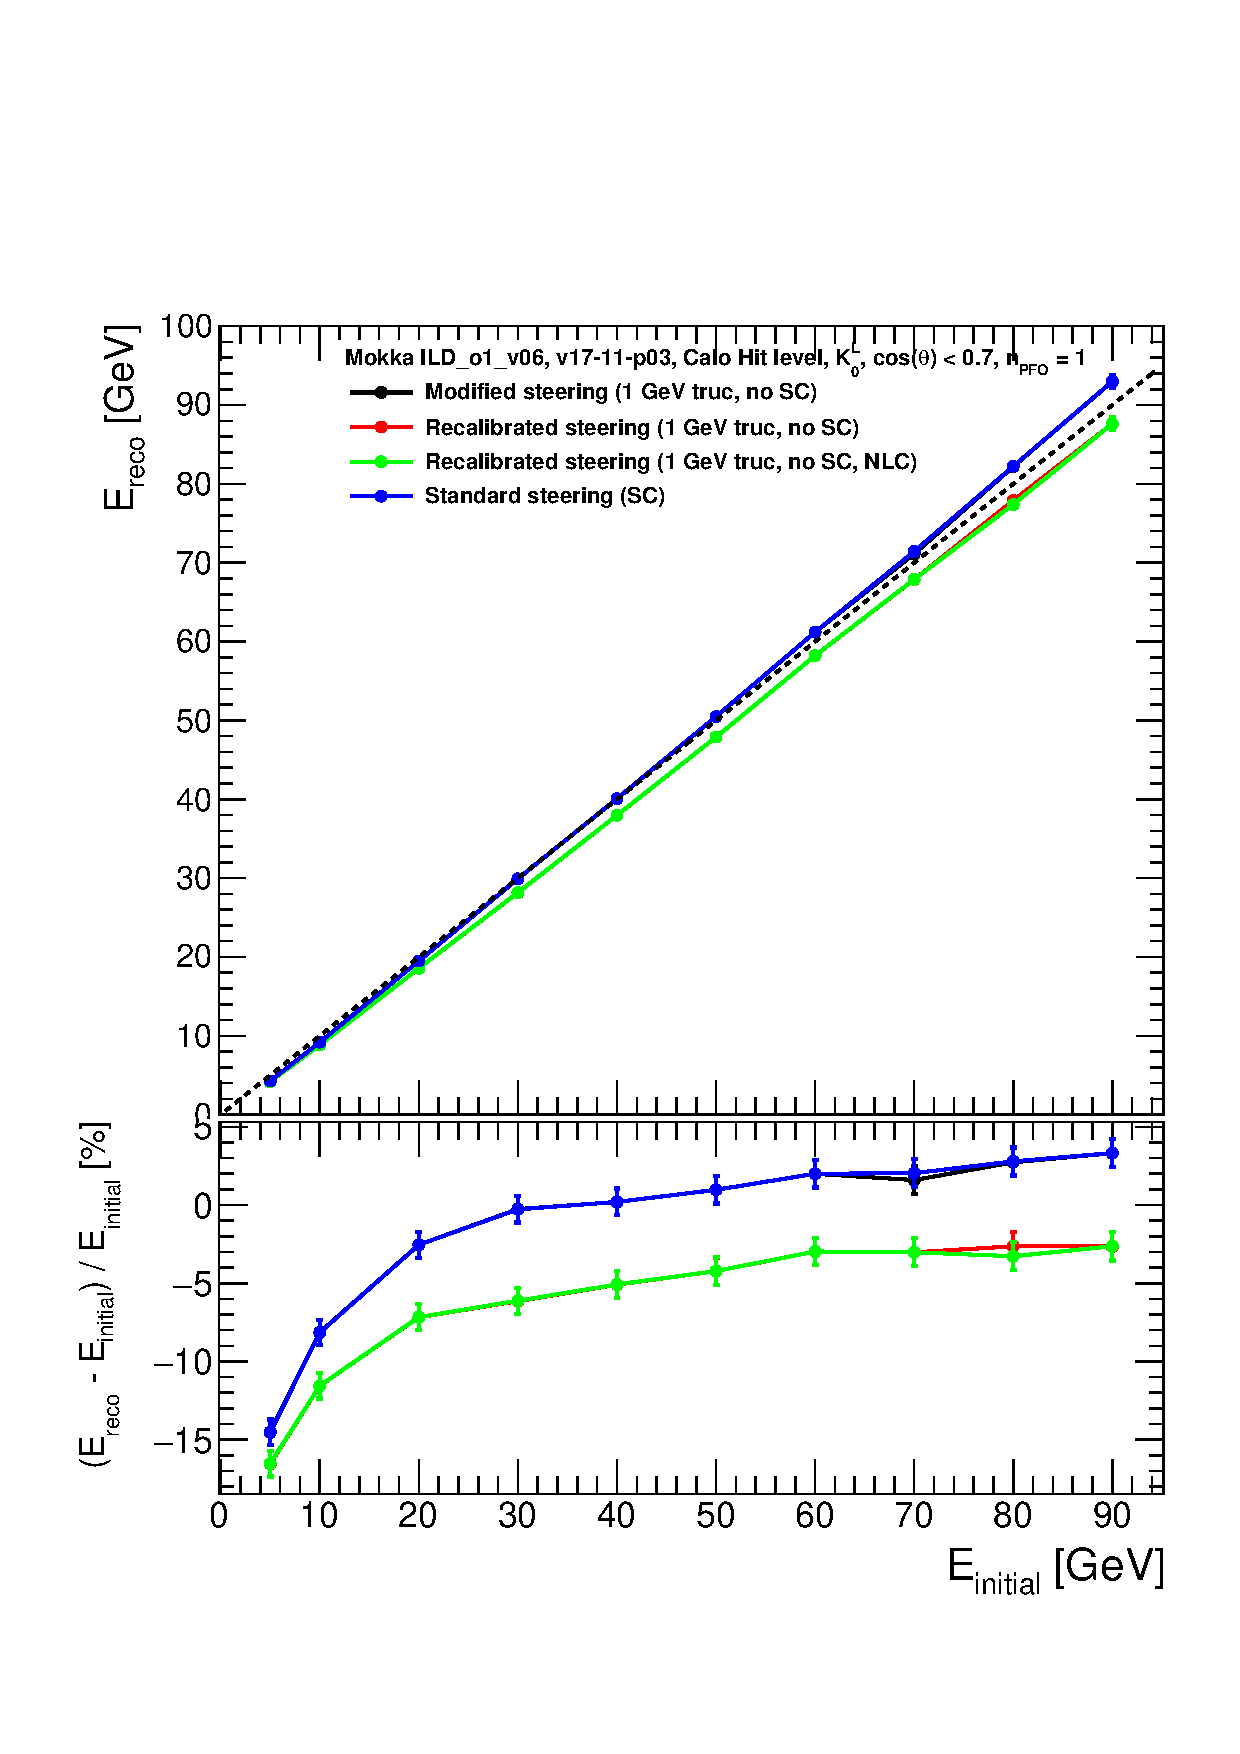
\includegraphics[width=0.7\linewidth]{../Thesis_Plots/ILD/NoSmearing/Plots_Comparison/Comparison_linearity_Curves_Hits}
  \caption{Mean energy $E_{reco}$ for 5 to 90 GeV \kzeroL{} as a function of the simulated energy $E_{initial}$ for different parameters in the reconstruction at the hit level. The bottom plot shows the relative deviation from linearity. Error bars represent the statistical uncertainty.} \label{fig:linhits}
\end{figure}

\begin{figure}[htbp!]
  \centering
  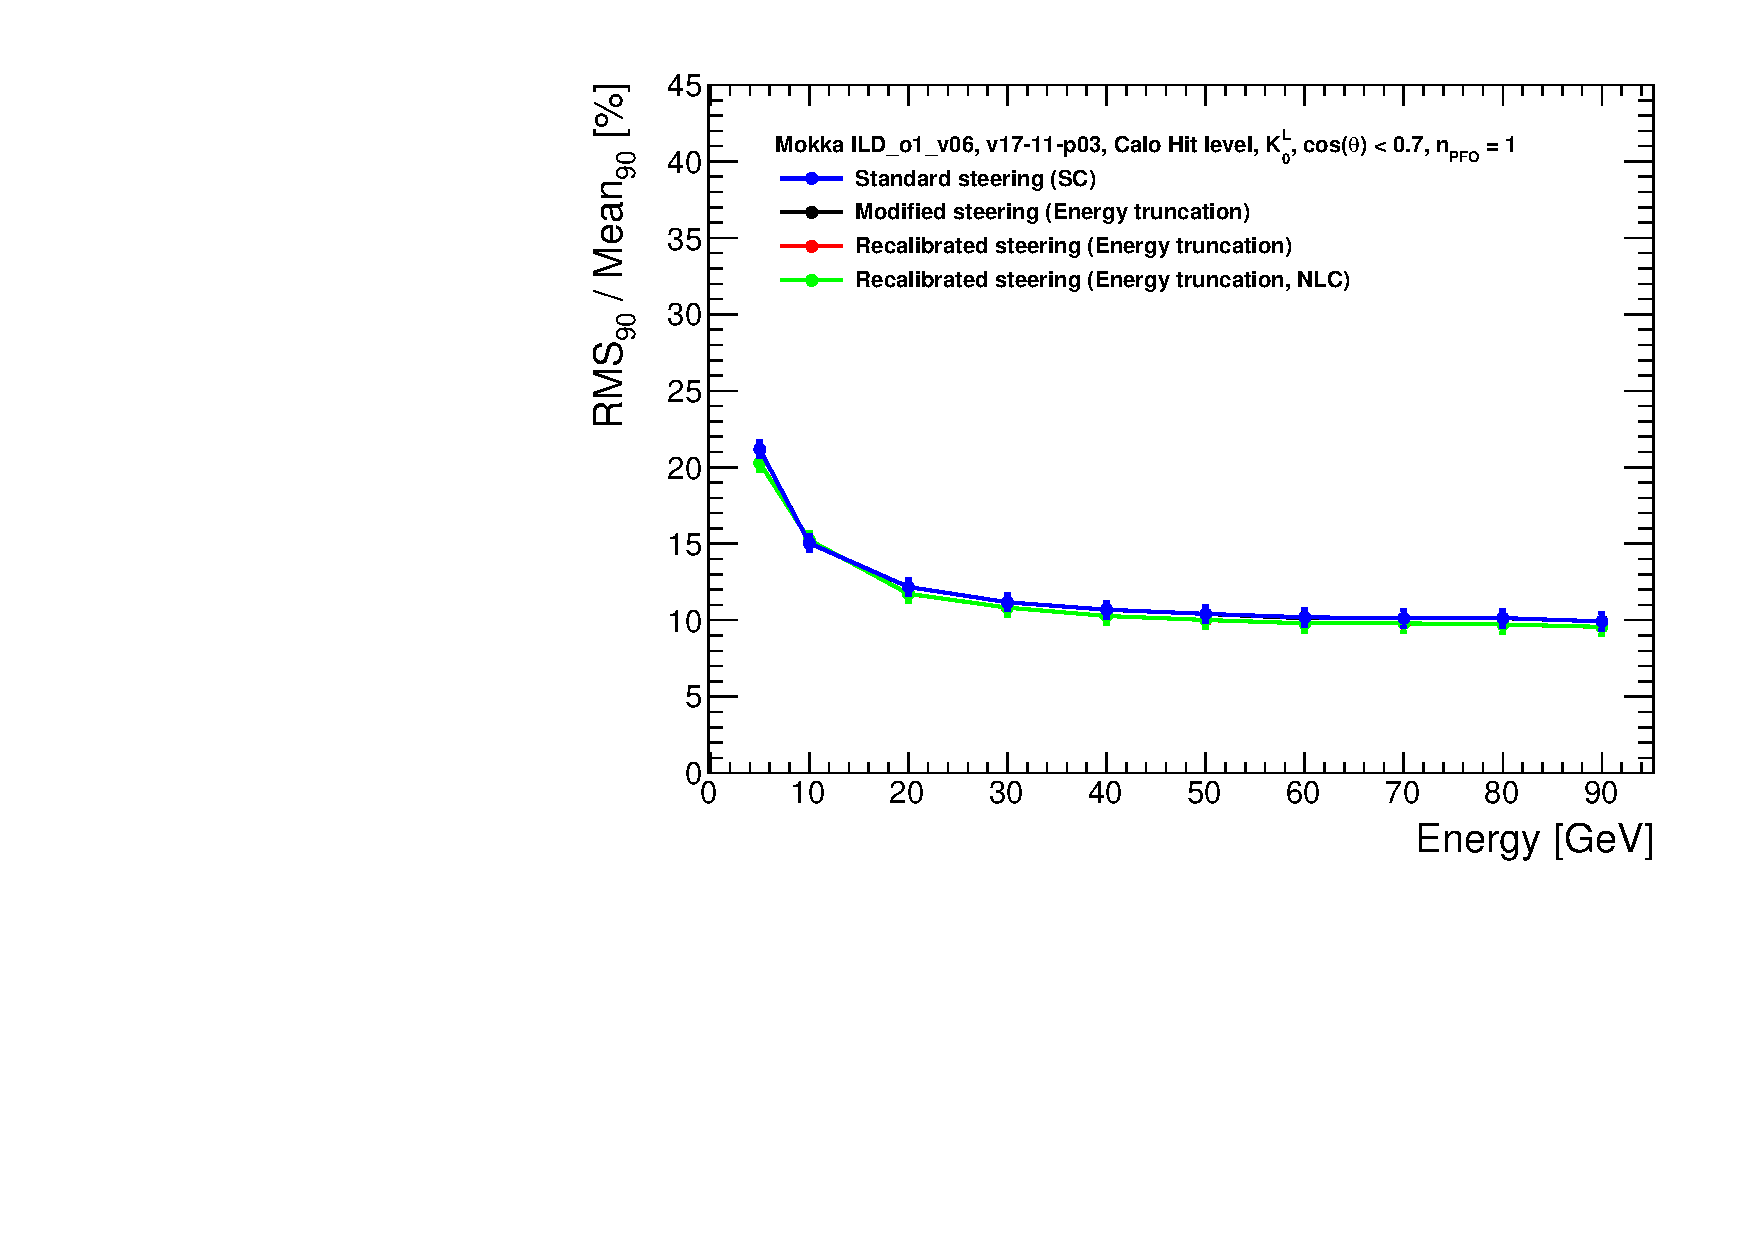
\includegraphics[width=0.7\linewidth]{../Thesis_Plots/ILD/NoSmearing/Plots_Comparison/Comparison_resolution_Curves_Hits}
  \caption{Relative energy resolution RMS$_{90}$/Mean$_{90}$ as a function of the energy for different parameters in the reconstruction at the hit level. Error bars represent the statistical uncertainty.} \label{fig:resohits}
\end{figure}

Another option is to look at the PFO level as shown in figures \ref{fig:linpfo} and \ref{fig:resopfo}. By looking at the difference between these figures and the figures \ref{fig:linhits} and \ref{fig:resohits}, one can understand the effects of the different configurations in PandoraPFA. For the linearity curve, the red and black line are quite similar and show a non-linearity especially at high energies between -10\% and 2\%. This shows that the energy truncation may introduce a non-linearity effect. The difference between the curves is only the constants used for the correction of the sampling fraction, it has also a small effect ($\sim$ 1-2\%) that may come from clustering.

The green line is linear due to the non-linearity correction. Finally, the blue line is off by around 10\%. This is believed to be due to the weights of the software compensation that are not optimal for this model.

For the resolution curves, a very small rise ($\sim$ 1-2\%) of the resolution at high energies for the modified and recalibrated configurations is visible. In the case where the non-linearity correction is performed, one can observe a degradation of the energy resolution as expected. In the case of software compensation, a change in the curve can be seen at 50 GeV. This is correlated with the change of the slope in the linearity plot.

\begin{figure}[htbp!]
  \centering
  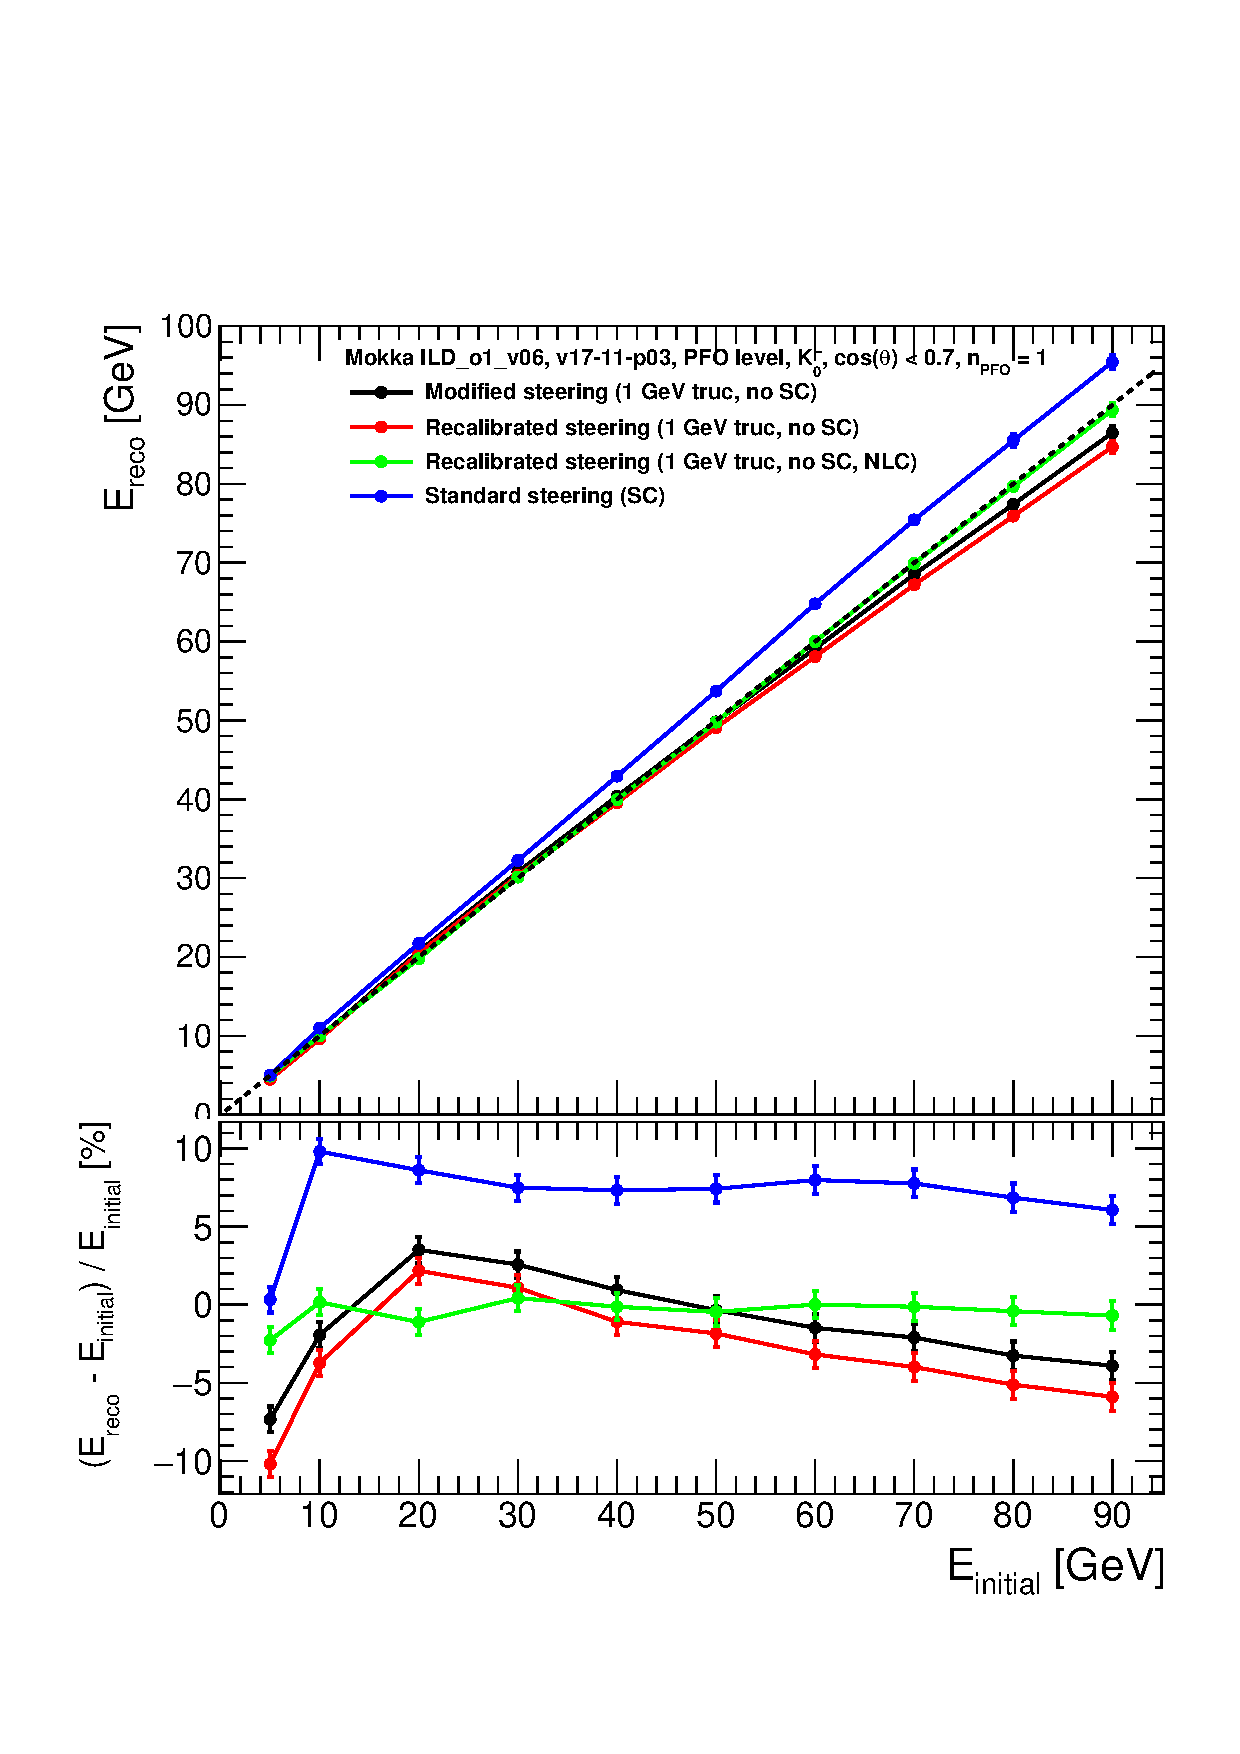
\includegraphics[width=0.7\linewidth]{../Thesis_Plots/ILD/NoSmearing/Plots_Comparison/Comparison_linearity_Curves_PFO}
  \caption{PFO linearity curve.} \label{fig:linpfo}
\end{figure}

\begin{figure}[htbp!]
  \centering
  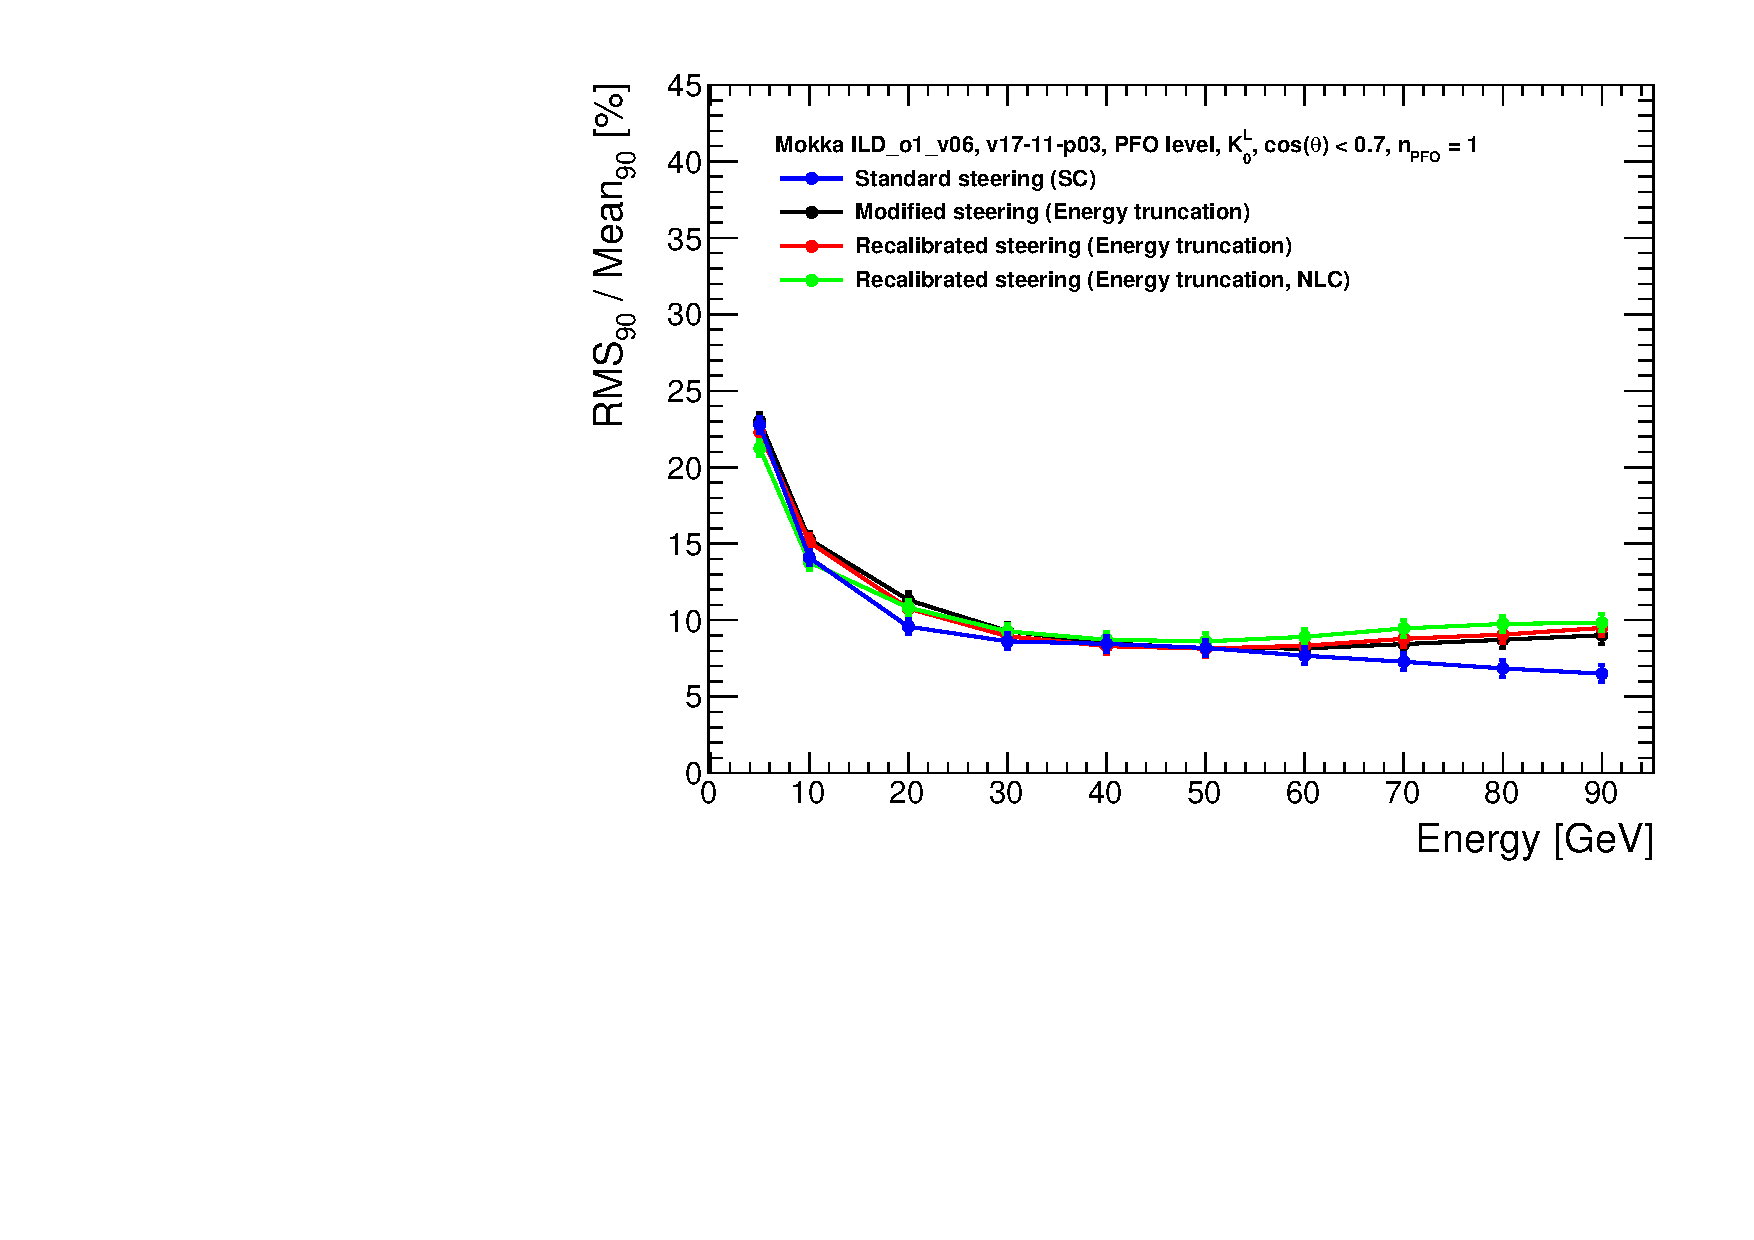
\includegraphics[width=0.7\linewidth]{../Thesis_Plots/ILD/NoSmearing/Plots_Comparison/Comparison_resolution_Curves_PFO}
  \caption{PFO resolution curve.} \label{fig:resopfo}
\end{figure}

Despite that the energy linearity is not perfect after the recalibration, it is verified that the calibration is correct. In the following subsections, I will look at only at the hit level in order to avoid clustering effects by PandoraPFA. Therefore, the recalibrated setting with energy truncation and non-linearity correction was chosen.

\subsection{Timing cut effects on hadronic showers in ILD detector}

Though the linearity is not perfect over all energies for single particles, the most regarded observable is the jet energy resolution. As explained in chapter \ref{sec:PFA}, jets have a large fraction of charged particles of around 60\%. In this case, the energy of the PFO is coming from the track. Moreover neutral particles (excluding photons) are counting in average for around 30\% of the contribution in a jet.

As shown in figure \ref{fig:momentumparticlejets}, for jets representative of heavy boson decay near production threshold, the momentum spectrum is dominant at around 10 \GeV as for heavy boosted jets with a more complex event topology, the momentum distribution is still dominant at low energies but presents a tail at much higher energies. Thus the non-linearity has only little effect there. It is still relevant to understand the different effects of the reconstruction at single-particle level.

\begin{figure}[htbp!]
  \centering
  \begin{subfigure}[t]{0.48\textwidth}
    \centering
    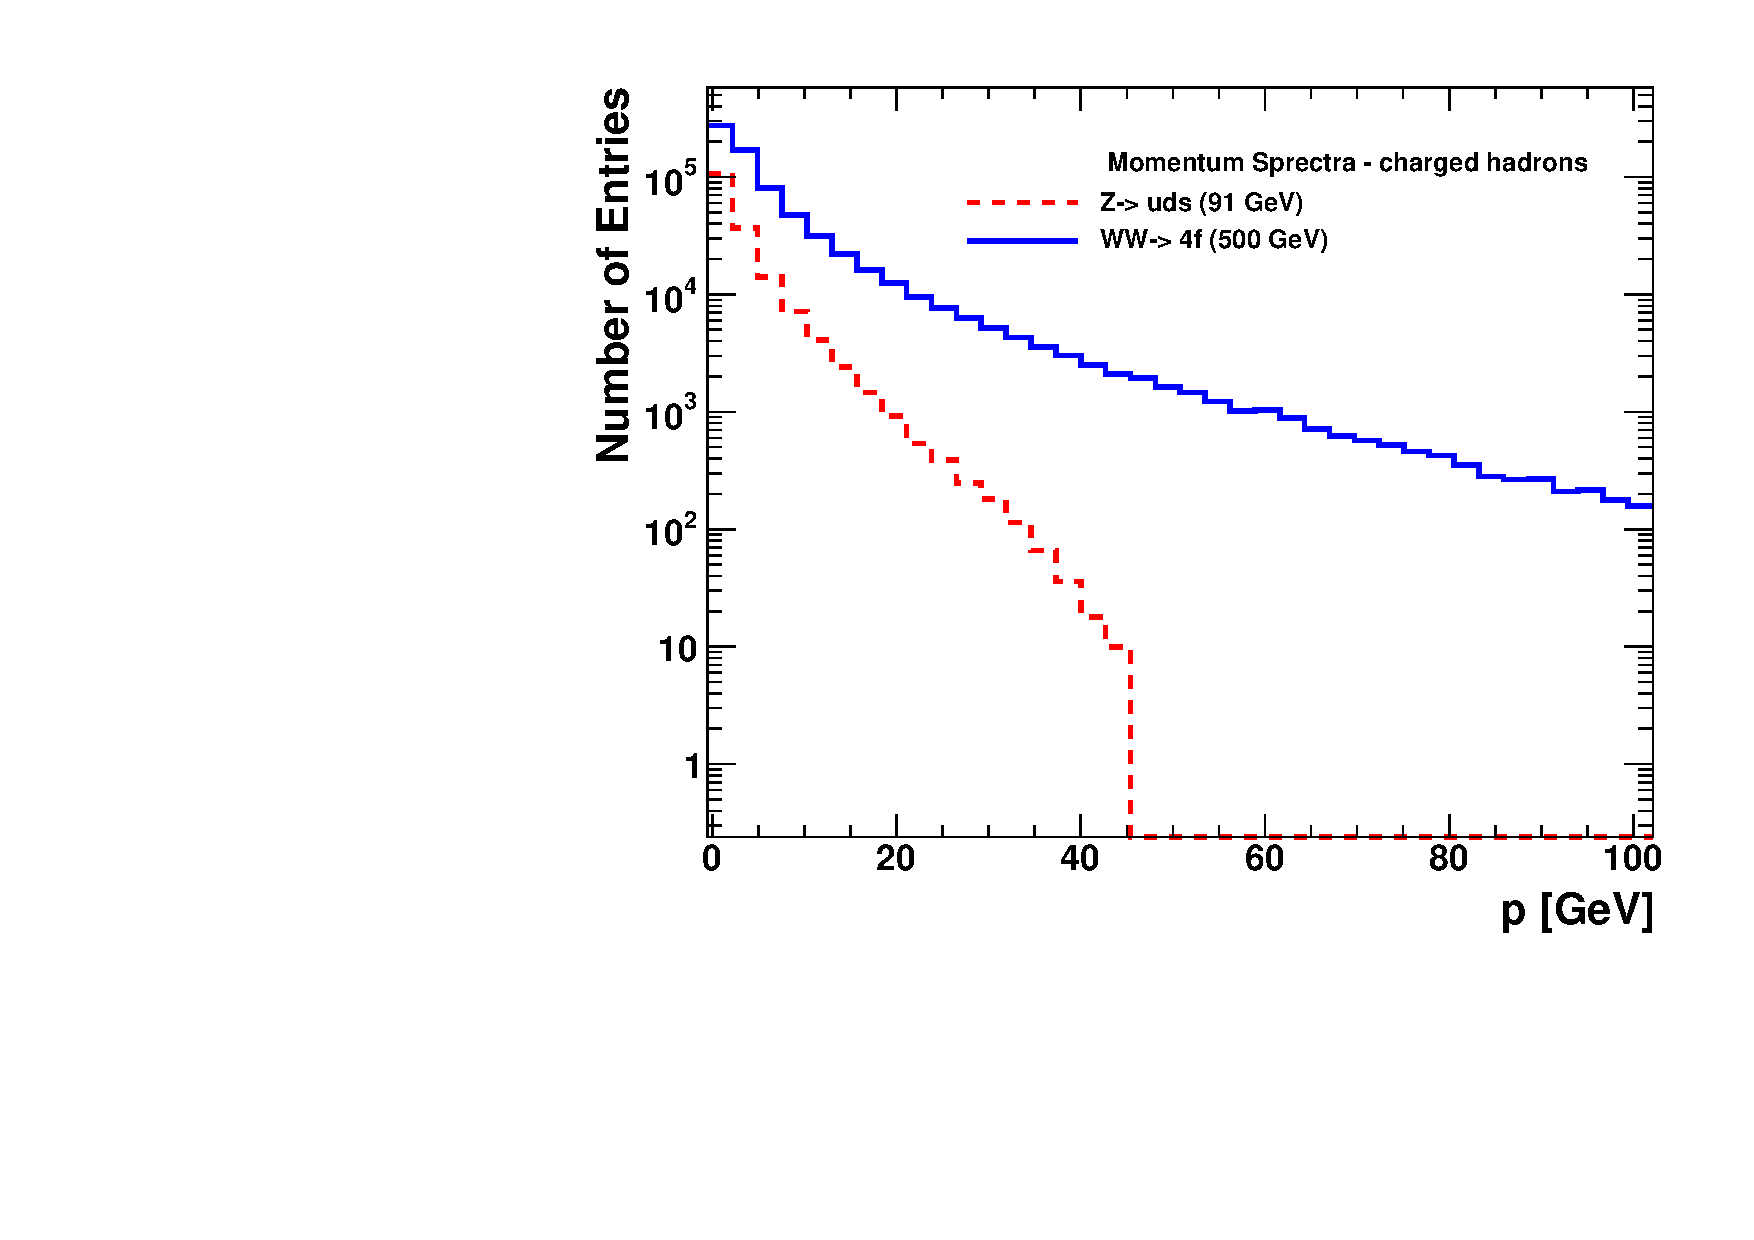
\includegraphics[width=1\linewidth]{../Thesis_Plots/ILD/Momentum_spectra_to100GeV_final}
    \caption{Momentum spectrum of charged hadrons.} \label{fig:momentumparticlejets}
  \end{subfigure}
  \begin{subfigure}[t]{0.48\textwidth}
    \centering
    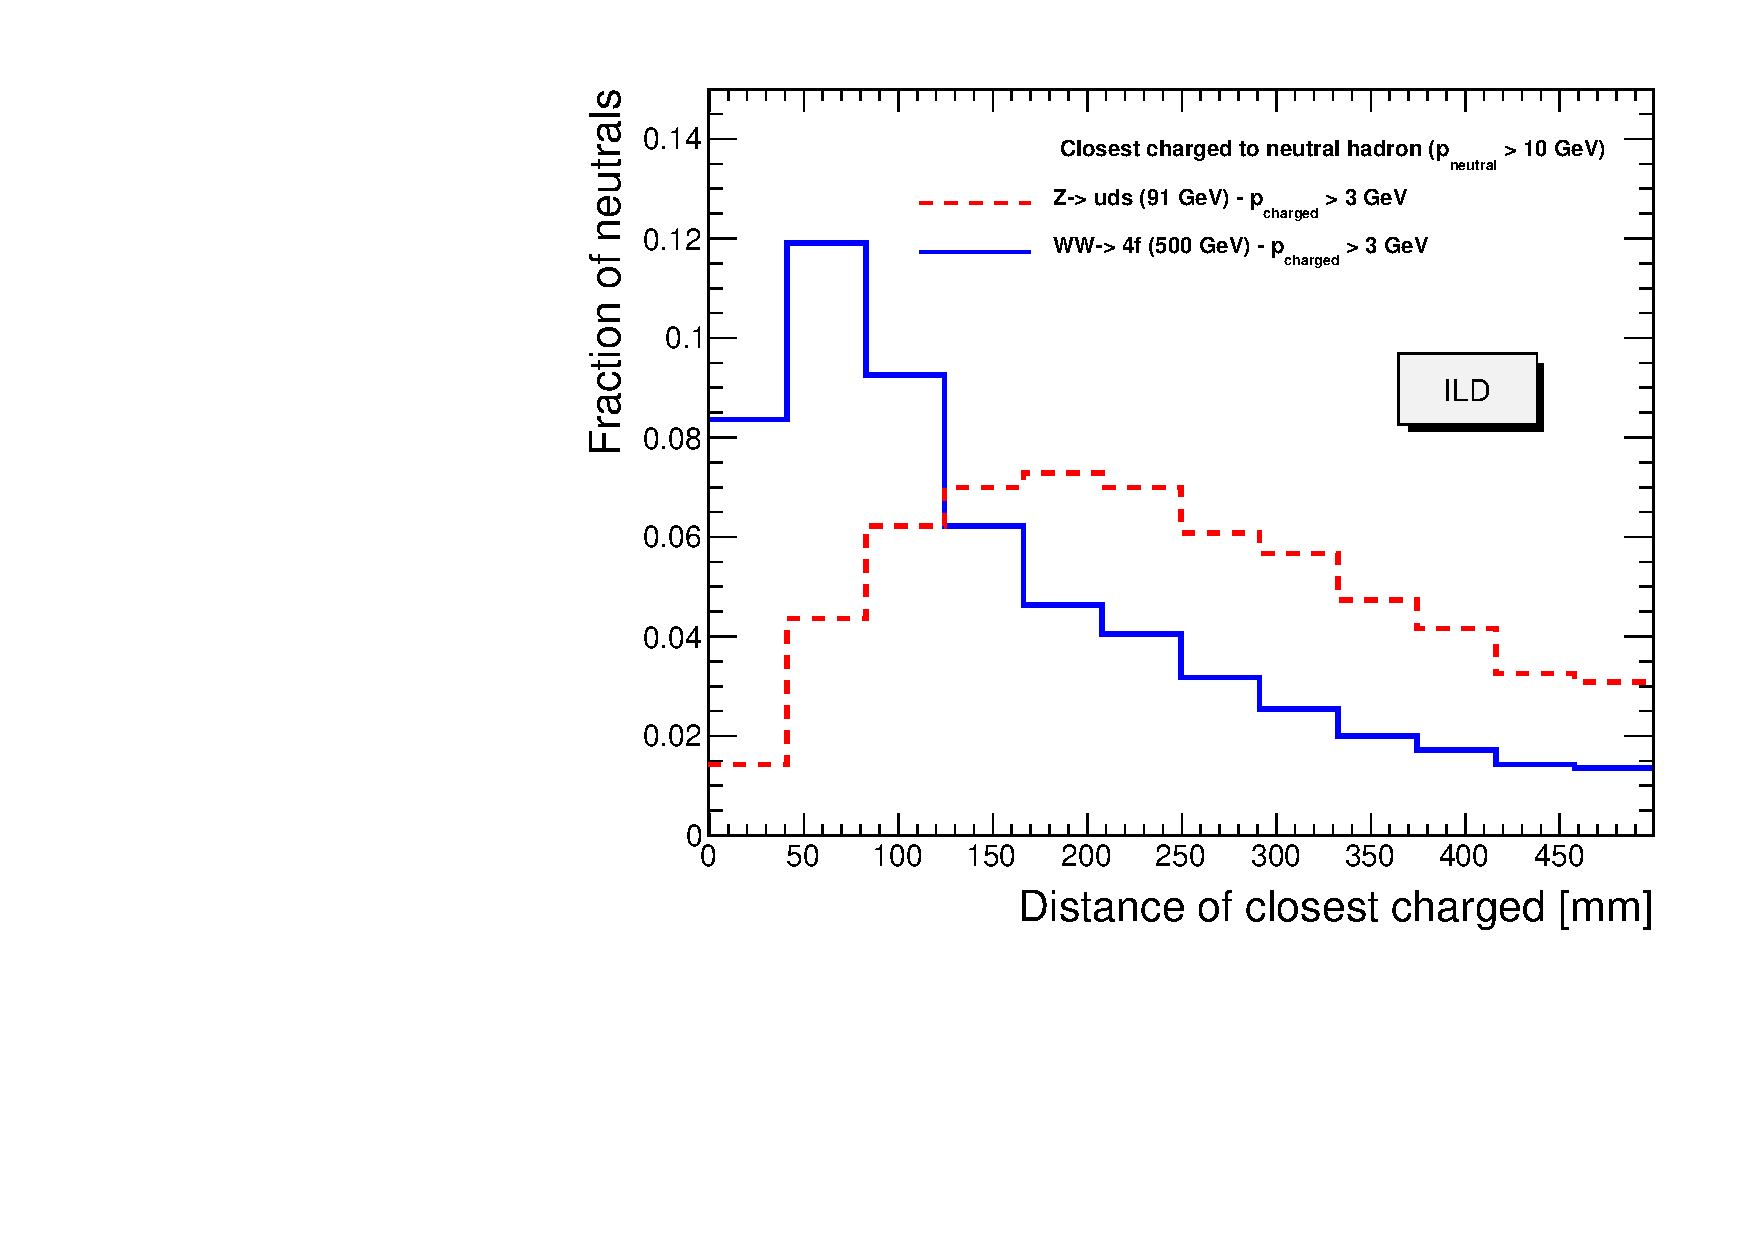
\includegraphics[width=1\linewidth]{../Thesis_Plots/ILD/Stackall_dmin_3GeVneu_10GeVcharged_final_3_morestat}
    \caption{Minimal distance between a charged and neutral particle at the front face of the ECAL.} \label{fig:distancefrontfacejets}
  \end{subfigure}
  \caption{\subref{fig:momentumparticlejets}) Momentum distribution for charged particles in simulated \ee{}\ra{} \Zqq{} with $q = u,d,s$ at \rts{} = 91 \GeV and \ee{}\ra{} \WWqqqq{} where q is a quark at \rts{} = 500 \GeV. \subref{fig:distancefrontfacejets}) Distribution of distances to the closest charged track for neutral particles produced in \Zqq{} and \WWqqqq{} processes measured at the front face of the electromagnetic calorimeter in the ILD detector.}
\end{figure}

A complementary study was to look at the minimal distance between a charged and neutral particle for different physics processes, a Z boson produced near threshold and more complex topological event with energetic jets. The figure \ref{fig:distancefrontfacejets} shows that for low energy jets the mean minimal distance (measured at the front face of the SiW-ECAL) between a charged and neutral hadron is around \SI{180}{\milli\meter} thus in this context, showers are well separated. But at higher energies where density is higher, typical distances of \SI{50}{\milli\meter} need to be resolved. This situation can become relevant in the contribution of confusion to the jet energy resolution. In this case, the use of timing information could help to separate nearby showers and improve the pattern recognition.

In this section, the effect of timing cuts on hadronic showers is investigated. The study was performed using the \ilcsoft framework for reconstruction. In order to study the effect of timing on hadronic shower properties, the initial study was performed assuming a perfect timing resolution (i.e. the timing information is the Monte-Carlo truth). In a following step, several timing resolutions were used to assess different scenarios. The smearing of the time was done by randomly sampling a normalized Gaussian centered at \SI{0}{\nano\second} with a timing resolution denoted $\sigma_{t}$ = 0.4, 1 and \SI{8}{\nano\second} only on HCAL hits.

\subsubsection{Event Selection}

A simple selection is performed in order to select only events showering in the HCAL similar as in \cite{SoftCompNew2012} and also contained to minimize leakage as the following:
\begin{itemize}
  \item $|cos\theta|$ < 0.7 (Only barrel)
  \item $E_{ECAL}/E_{tot}$ < 5\%
  \item Shower start in first 5 layers of HCAL
\end{itemize}

\subsubsection{Impact on Particle Flow Objects (PFOs) reconstruction}

At first, the impact of timing cuts on the number of reconstructed particles was investigated. The figure \ref{fig:DistriPFO} shows the number of reconstructed PFO per event for different timing cuts.

\begin{figure}[htbp!]
  \centering
  \begin{subfigure}[t]{0.49\textwidth}
    \centering
    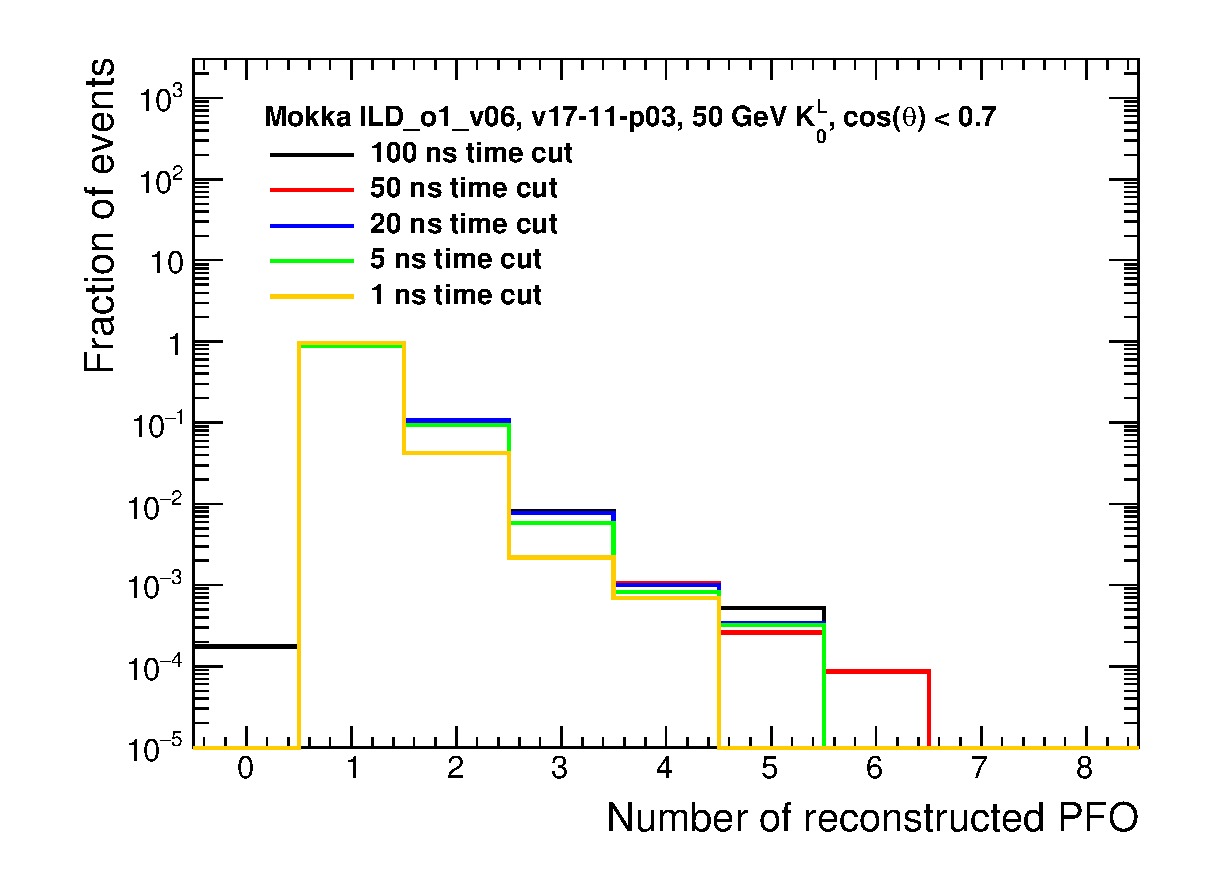
\includegraphics[width=1\linewidth]{../Thesis_Plots/ILD/AdditionalPlots/Plots/NumberReconstructedPFO_TimeCuts_50GeV}
    \caption{Number of reconstructed PFO per event.} \label{fig:DistriPFO}
  \end{subfigure}
  \begin{subfigure}[t]{0.49\textwidth}
    \centering
    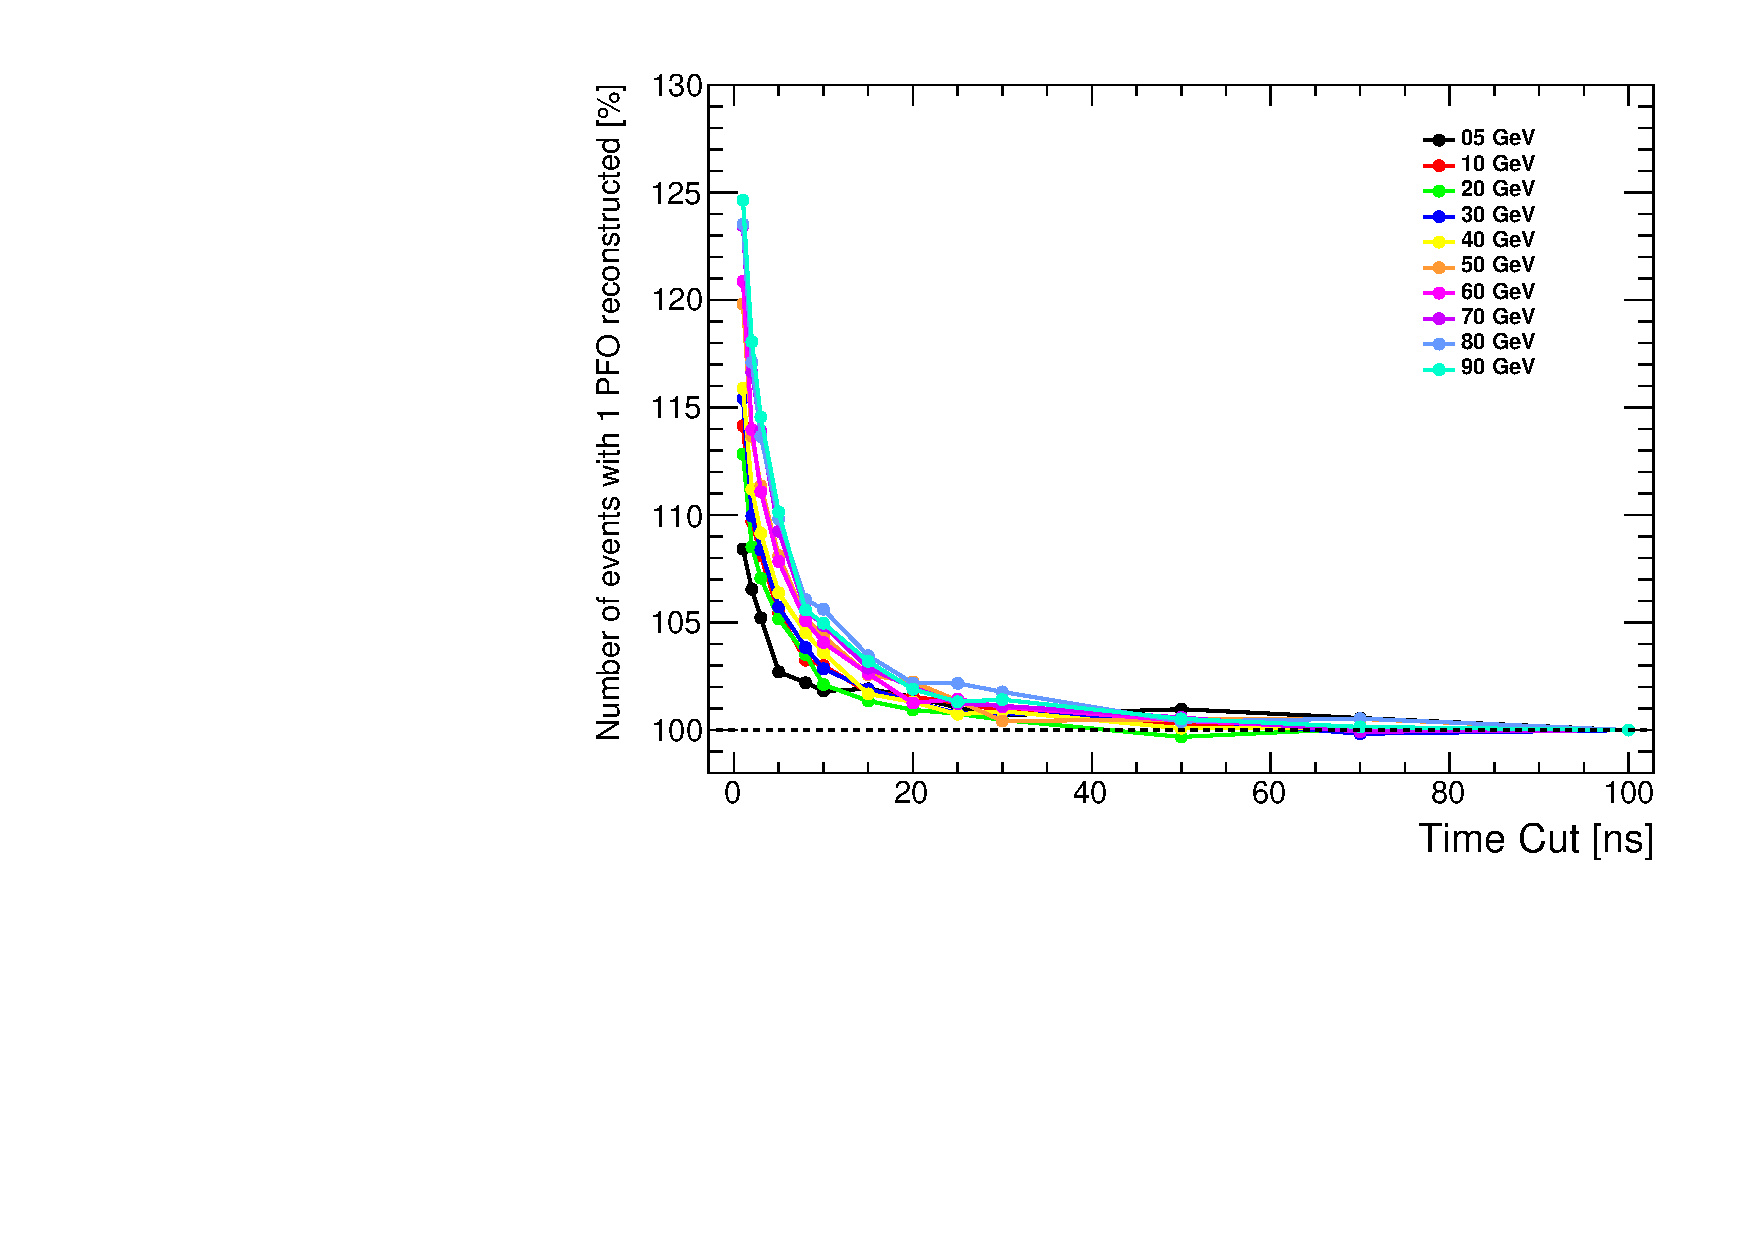
\includegraphics[width=1\linewidth]{../Thesis_Plots/ILD/NoSmearing/Plots/NumberEvents_PFO_TimeCuts_noSmearing}
    \caption{Relative number of events reconstructed with a single PFO.} \label{fig:EventRecoPFO}
  \end{subfigure}
  \caption{\subref{fig:DistriPFO}) Distribution of the number of PFO reconstructed per event for 50 GeV \kzeroL{} in the ILD barrel for different timing cuts. It shows that timing cuts indeed improves the number of events reconstructed with a single PFO but as well a large tail is present. The use of timing cuts reduces slightly the tail of the distribution. \subref{fig:EventRecoPFO}) The plot shows the number of events reconstructed with only a single PFO normalized to the number of events in the case of 100 ns. It shows a relative increase with a lower timing cut, up to 20-25\% more events reconstructed using 1 ns timing cut.}
\end{figure}

One can notice that more events are indeed reconstructed with a single PFO but a tail is present to higher number of reconstructed PFOs in all distributions. Up to 4-5 PFOs can be reconstructed in a single event though it is at a per-mil level. It demonstrates that timing cuts reduces the number of events reconstructed with more than one PFO. Therefore, this has been look at for all energies between 5 and 90 GeV. The figure \ref{fig:EventRecoPFO} shows the number of events reconstructed with a single PFO relative to the default configuration with 100 ns timing cut. Timing cuts increase the fraction of reconstructed events containing a single PFO over all energies up to 20-25\% for the highest particle energies.

To understand more into details what happens, a look at the energy distribution and distance of the second most energetic cluster to the main cluster has been performed in the case of more than one PFO is reconstructed. It can be seen on figures \ref{fig:Energy2ndCluster} and \ref{fig:Distance2ndCluster} for 50 GeV \kzeroL{} for different timing cuts of 100 ns and 1 ns.

\begin{figure}[htbp!]
  \centering
  \begin{subfigure}[t]{0.49\textwidth}
    \centering
    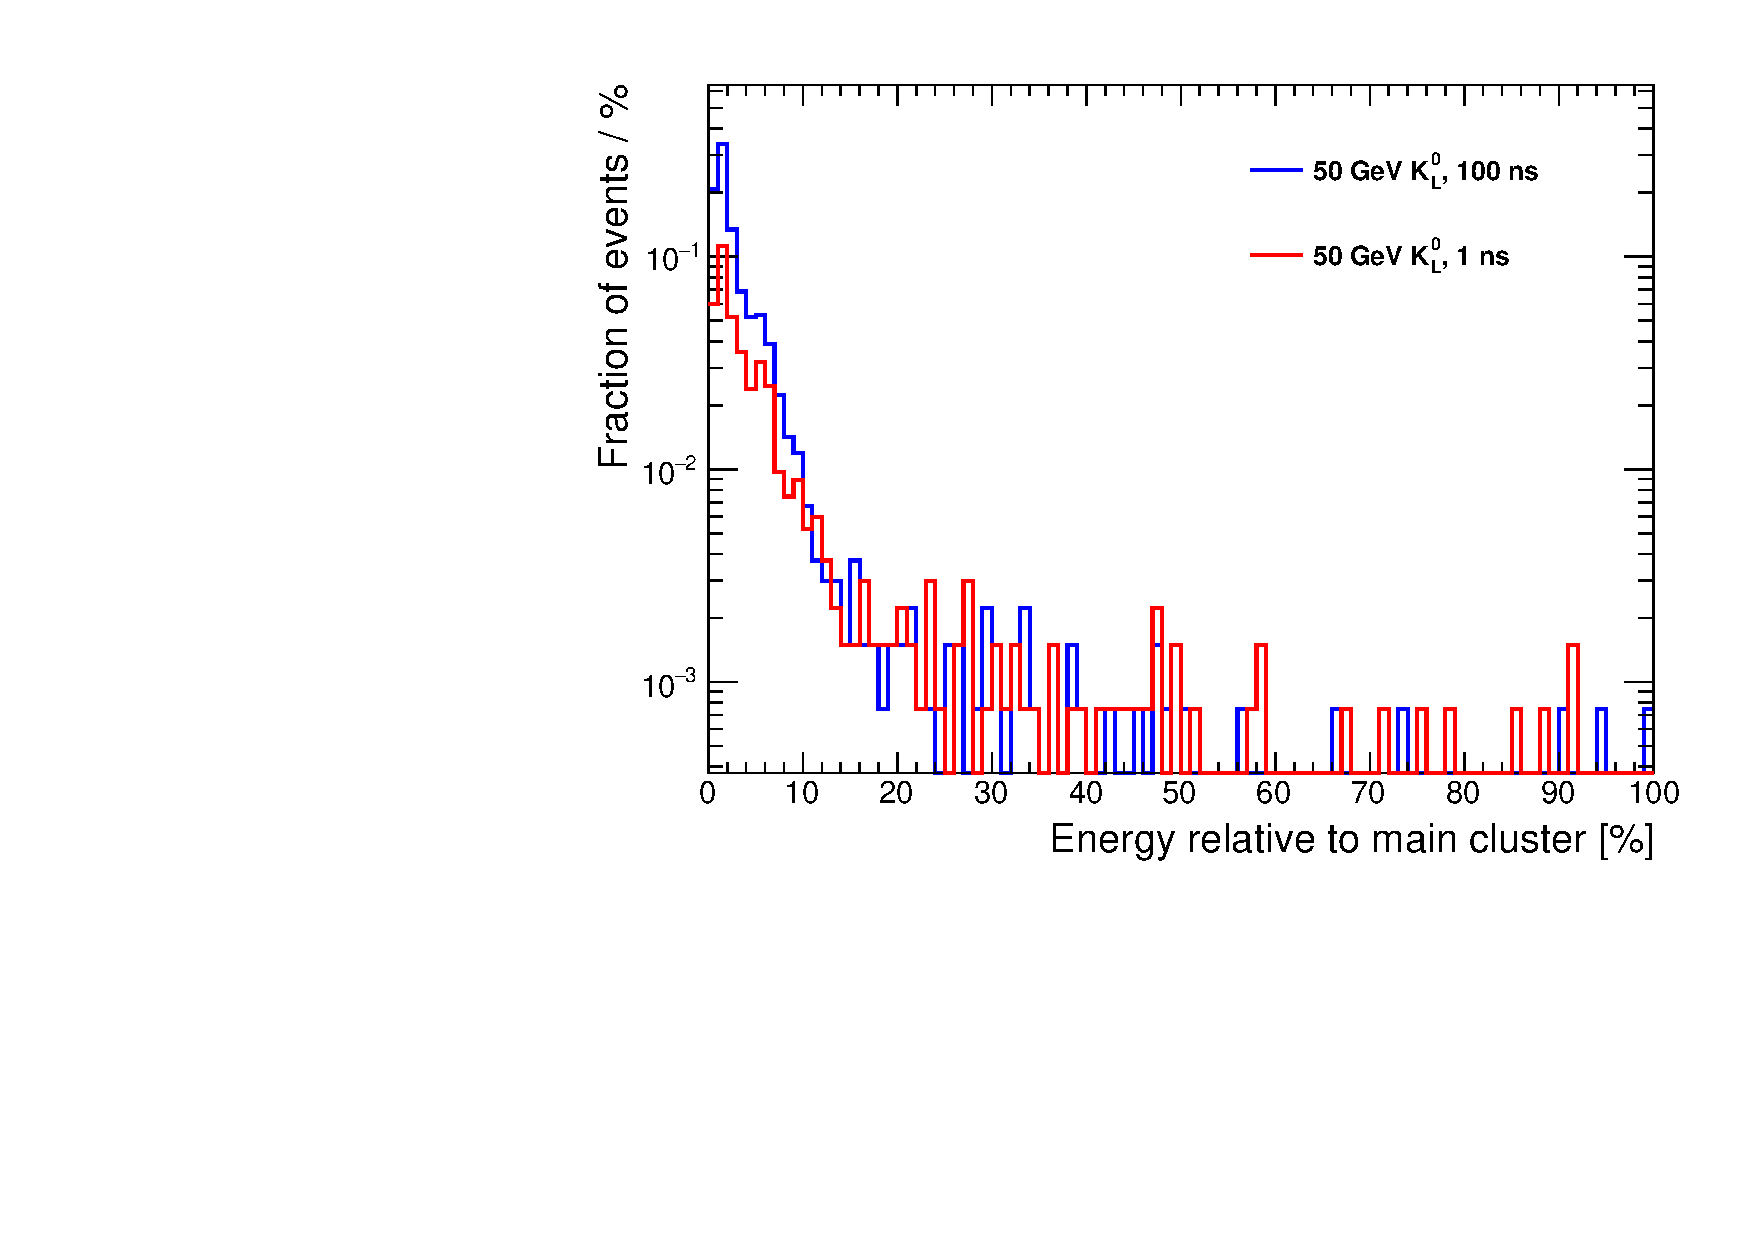
\includegraphics[width=1\linewidth]{../Thesis_Plots/ILD/AdditionalPlots/Plots/Energy2ndCluster_100ns_50GeV}
    \caption{Energy distribution of 2$^{nd}$ most energetic cluster normalized to the number of events at 100 ns.} \label{fig:Energy2ndCluster}
  \end{subfigure}
  \hfill
  \begin{subfigure}[t]{0.49\textwidth}
    \centering
    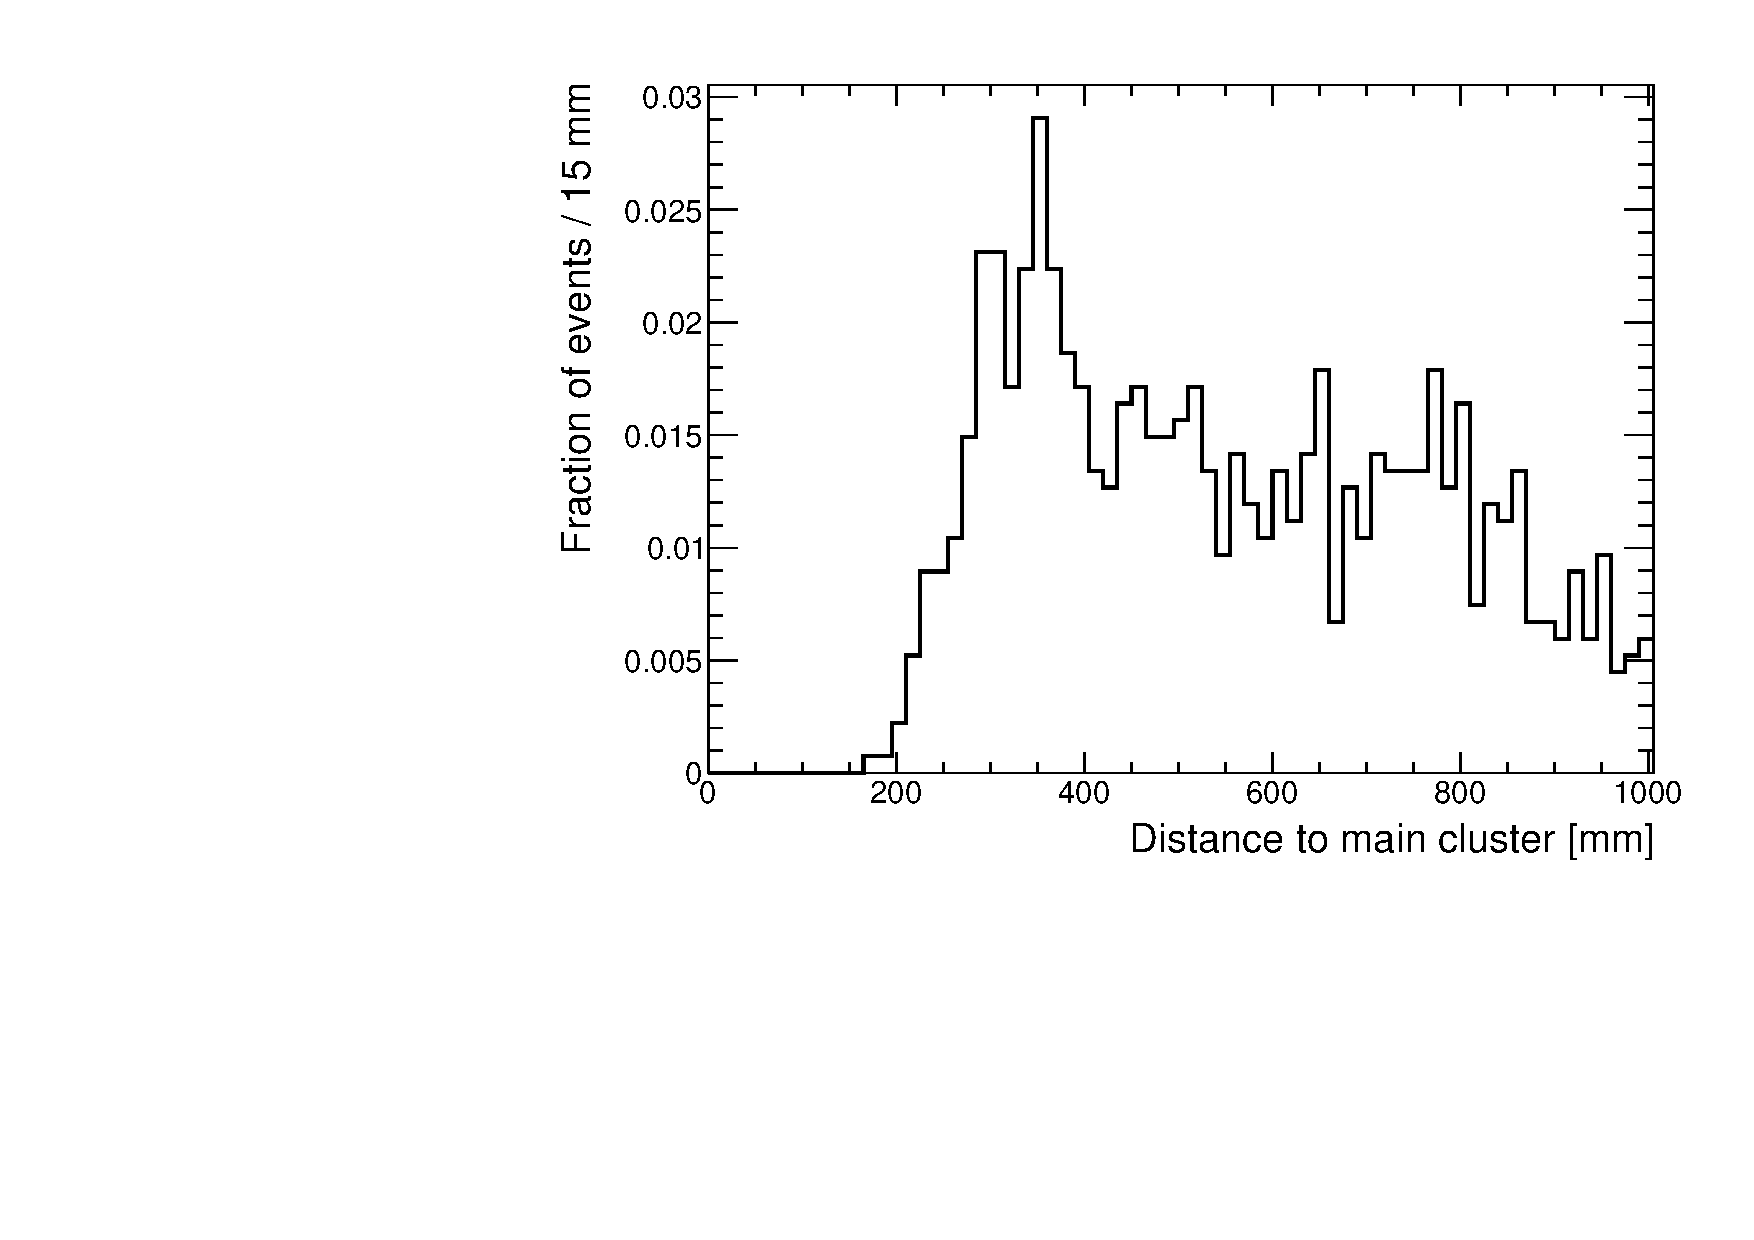
\includegraphics[width=1\linewidth]{../Thesis_Plots/ILD/AdditionalPlots/Plots/Distance2ndCluster_100ns_50GeV}
    \caption{Distance to main PFO of 2$^{nd}$ most energetic cluster normalized to the number of events at 100 ns.} \label{fig:Distance2ndCluster}
  \end{subfigure}
  \caption{\subref{fig:Energy2ndCluster}) The plot shows the relative energy of the second most energetic cluster to the main cluster. One can see that most of the entries are below few percents. \subref{fig:Distance2ndCluster}) The plot shows the distribution of the distance of the second most energetic cluster to the main cluster. The distribution peaks in the region 25-30 cm.}
\end{figure}

The figures show that the second most energetic cluster has mostly an energy below few percents, over 97\% of the entries are below 20\% of the most energetic cluster. The mean distance of this second cluster is around 25-30 cm from the main cluster with around 22\% of entries below 40 cm and is comprised of a long tail to higher distances. This is visible for both timing cuts of 100 ns and 1 ns. This tells us that mainly the split cluster has little energy compared to the main cluster and is situated at around 7 to 10 AHCAL tiles away from the main cluster which is far enough to not be recombined by Pandora with the main cluster. These clusters may be coming from low energy neutrons traveling through the calorimeter. This explains why by introducing a timing cut more events are reconstructed with a single PFO, as shown in chapter \ref{chap:TimingAHCAL}, low energy neutrons are correlated with low energy deposition and late depositions far away from the shower axis and are removed with a timing cut below few tens of nanoseconds.

One interesting point though would be the investigation of timing cuts in the case of overlapping showers in the calorimeter where timing could have the potential to improve separation between showers.

\subsection{Assuming perfect timing resolution}
\label{sec:MCLevelILDTiming}

The following section presents results of timing cuts assuming a perfect time resolution. To avoid any effects of clustering and Pandora, the study was performed at the calorimeter hit level. Several shower observables were looked at as a function of the time cut for energies from 5 \GeV to 90 \GeV \kzeroL. The different time cuts used are: 1, 2, 3, 5, 8, 10, 15, 20, 25, 30, 50, 70 and \SI{100}{\nano\second}.

The figures \ref{fig:linearityNoSmearing} and \ref{fig:resoNoSmearing} show the effect of the timing cut on linearity and energy resolution. The tighter the timing cut gets, the linearity slope decreases and resolution gets degraded. The linearity degrades as much as 10\% at high energies for a 1 ns timing cut. This effectively means that with a harder timing cut, more hits of the shower are removed but mostly only outer hits carrying only a small fraction of the total shower energy, the core of the shower mostly does not get affected by timing cut up to few nanoseconds as shown in figure \ref{fig:RadialProfNoSmearing}.

\begin{figure}[htbp!]
  \centering
  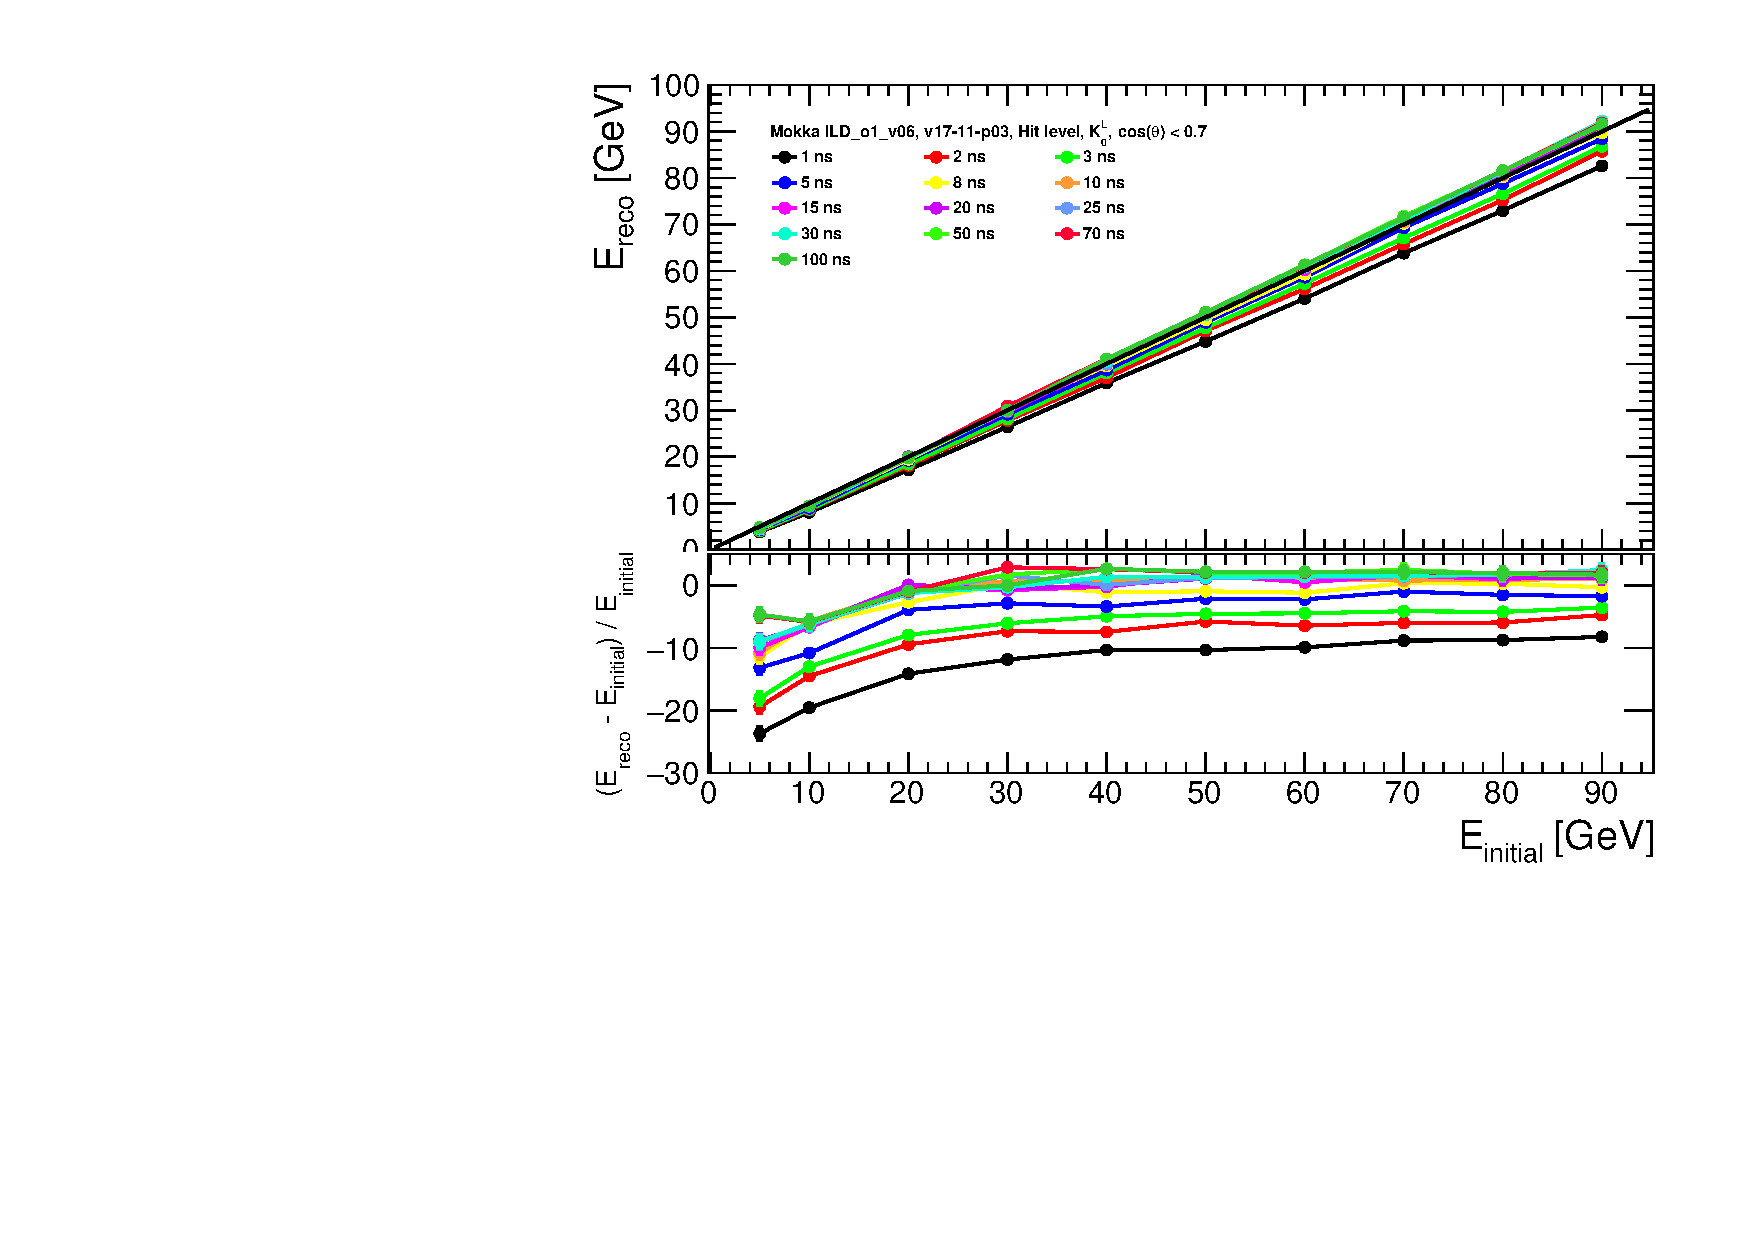
\includegraphics[width=0.7\linewidth]{../Thesis_Plots/ILD/NoSmearing/Plots/Linearity_TimeCuts_noSmearing}
  \caption{The top plot represent the linearity curve in the ILD detector over a range of energy from 5 \GeV to 90 \GeV for different timing cuts assuming a perfect resolution. The bottom plot represent the relative deviation to the line $x=y$ for the different time cuts.} \label{fig:linearityNoSmearing}
\end{figure}

The figure \ref{fig:resoNoSmearing} shows the relative impact on the energy resolution compared to the \SI{100}{\nano\second} cut as function of timing cuts for all energies. The energy resolution is very little affected for a cut of obove \SI{20}{\nano\second} meaning that the removed hits are not carrying a lot of energy and are part of the shower halo. Then below \SI{20}{\nano\second}, the resolution starts to degrade slowly relatively in the same way for all energies. A hard cut of 1 ns will degrade greatly the energy resolution up to around 20-30\%.

\begin{figure}[htbp!]
  \centering
  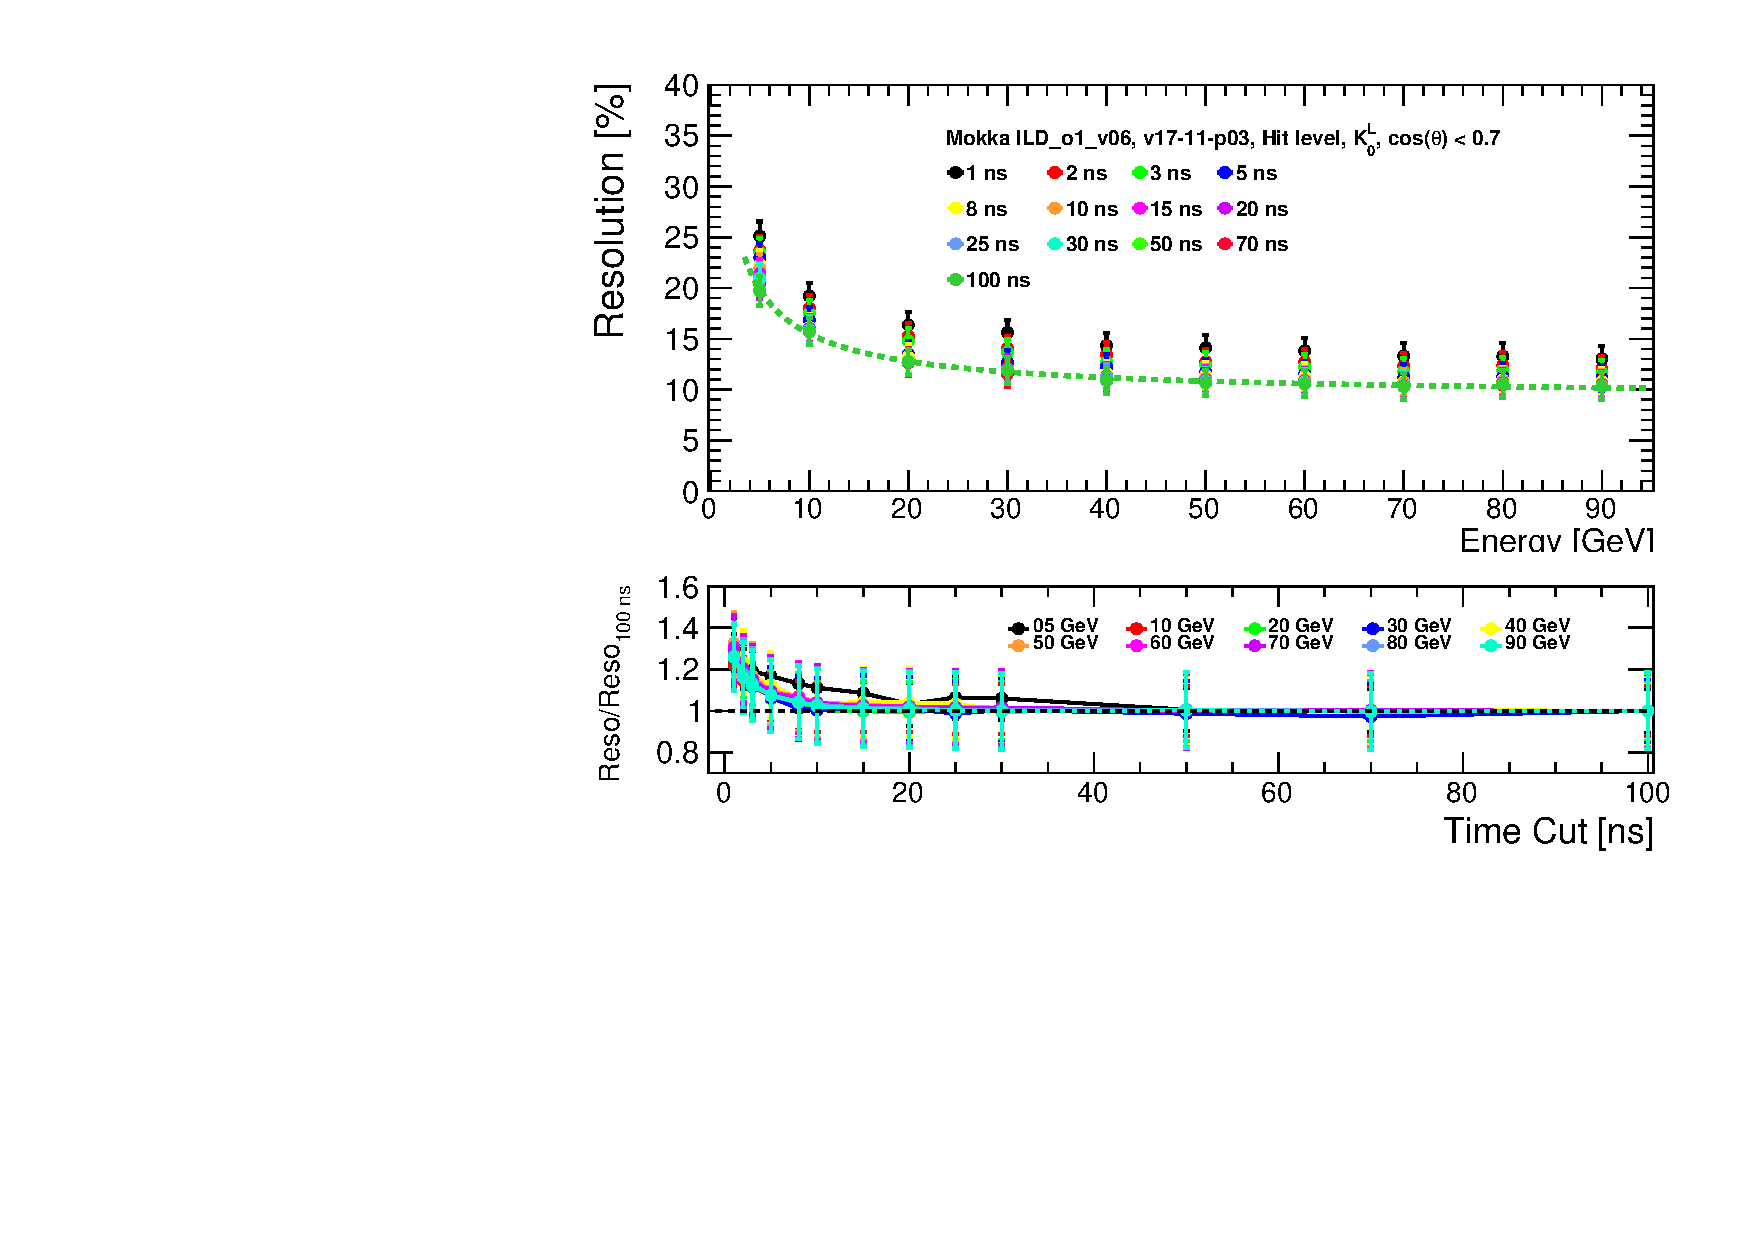
\includegraphics[width=0.7\linewidth]{../Thesis_Plots/ILD/NoSmearing/Plots/ShowerResoAbsolute_TimeCuts_noSmearing}
  \caption{The top plot illustrates the relative energy resolution ($\frac{\sigma_{E}}{E}$) at single particle level for different timing cuts. The green line is a fit performed at \SI{100}{\nano\second} of the form $\frac{\sigma_{E}}{E} = \frac{a}{\sqrt{E}} \bigoplus b$ where $a$ is the stochastic term ($39.14\% \pm 3.49$) and $b$ the constant term ($9.39\% \pm 0.70$). The bottom plot shows the relative change of the energy resolution compared to \SI{100}{\nano\second} as function of the timing cut for each particle energy. The error bars represent the statistical uncertainty.} \label{fig:resoNoSmearing}
\end{figure}

One can observe that the energy resolution degrades rapidly and faster than the energy of the shower. Naively, you would expect that if for example randomly 10\% of the shower energy is removed in average that then the resolution would behave as $\sqrt{E}$ and would degrade by around 6\% from a statistical point of view. But a timing cut does not remove hits randomly. It has a bias to remove late hits which are mostly coming from the hadronic component of the shower. As in hadronic showers, the electromagnetic and hadronic fraction of the shower is fluctuating a lot on an event-by-event basis this may affect the energy resolution much more. To understand this effect, a similar study as in \cite{SoftCompNew2012} has been performed in section \ref{sec:eresdegrad}.

The figure \ref{fig:RadialProfNoSmearing} shows the radial profile of a 50 \GeV hadronic shower. The radial profile of the shower is filled for each hit with the distance to the main shower axis ($R_{i}$, eq.\ref{eq:radialprof})  weighted by the hit energy ($E_{i}$).

\begin{equation} \label{eq:radialprof}
  \begin{split}
    & R_{i} = \sqrt{\Sigma_{i} (r_{i} - r_{cog})^{2} - \lVert (\mathbf{r_{i}} - \mathbf{r_{cog}}) \cdot \mathbf{Eigen} \rVert^{2}}) \\
    & \text{with} \quad \mathbf{r_{i}} = (x_i, y_i, z_i) \quad \text{and} \quad \mathbf{r_{CoG}} = (cog_x, cog_y, cog_z)
  \end{split}
\end{equation}

with $x_i, y_i, z_i$ the hit position, $cog_x, cog_y, cog_z$ the coordinates of the center of gravity of the shower and $\mathbf{Eigen}$ the eigenvector (main axis) of the shower. The main part of the energy density is situated in the core within few centimeters. The influence of timing cuts is highly visible in the tail of the distribution (or halo of the shower) and has little influence on the energy density deposited in the core of the shower. To quantify, a cut at 1 ns reduces up to 30\% the radial profile above 30-40 cm. An effect of an increase of energy density in the two first bins of the distribution is visible. This effect is related to a displacement of the center of gravity (CoG) as function of the timing cut as outer hits of the shower are removed. This has been checked by looking at the hit radius distribution relative to a fixed reference instead of the CoG (the Monte-Carlo particle endpoint). One can observe that in this case, the timing cut removes only part of the tail and does not affect the core of the distribution.

\begin{figure}[htbp!]
  \centering
  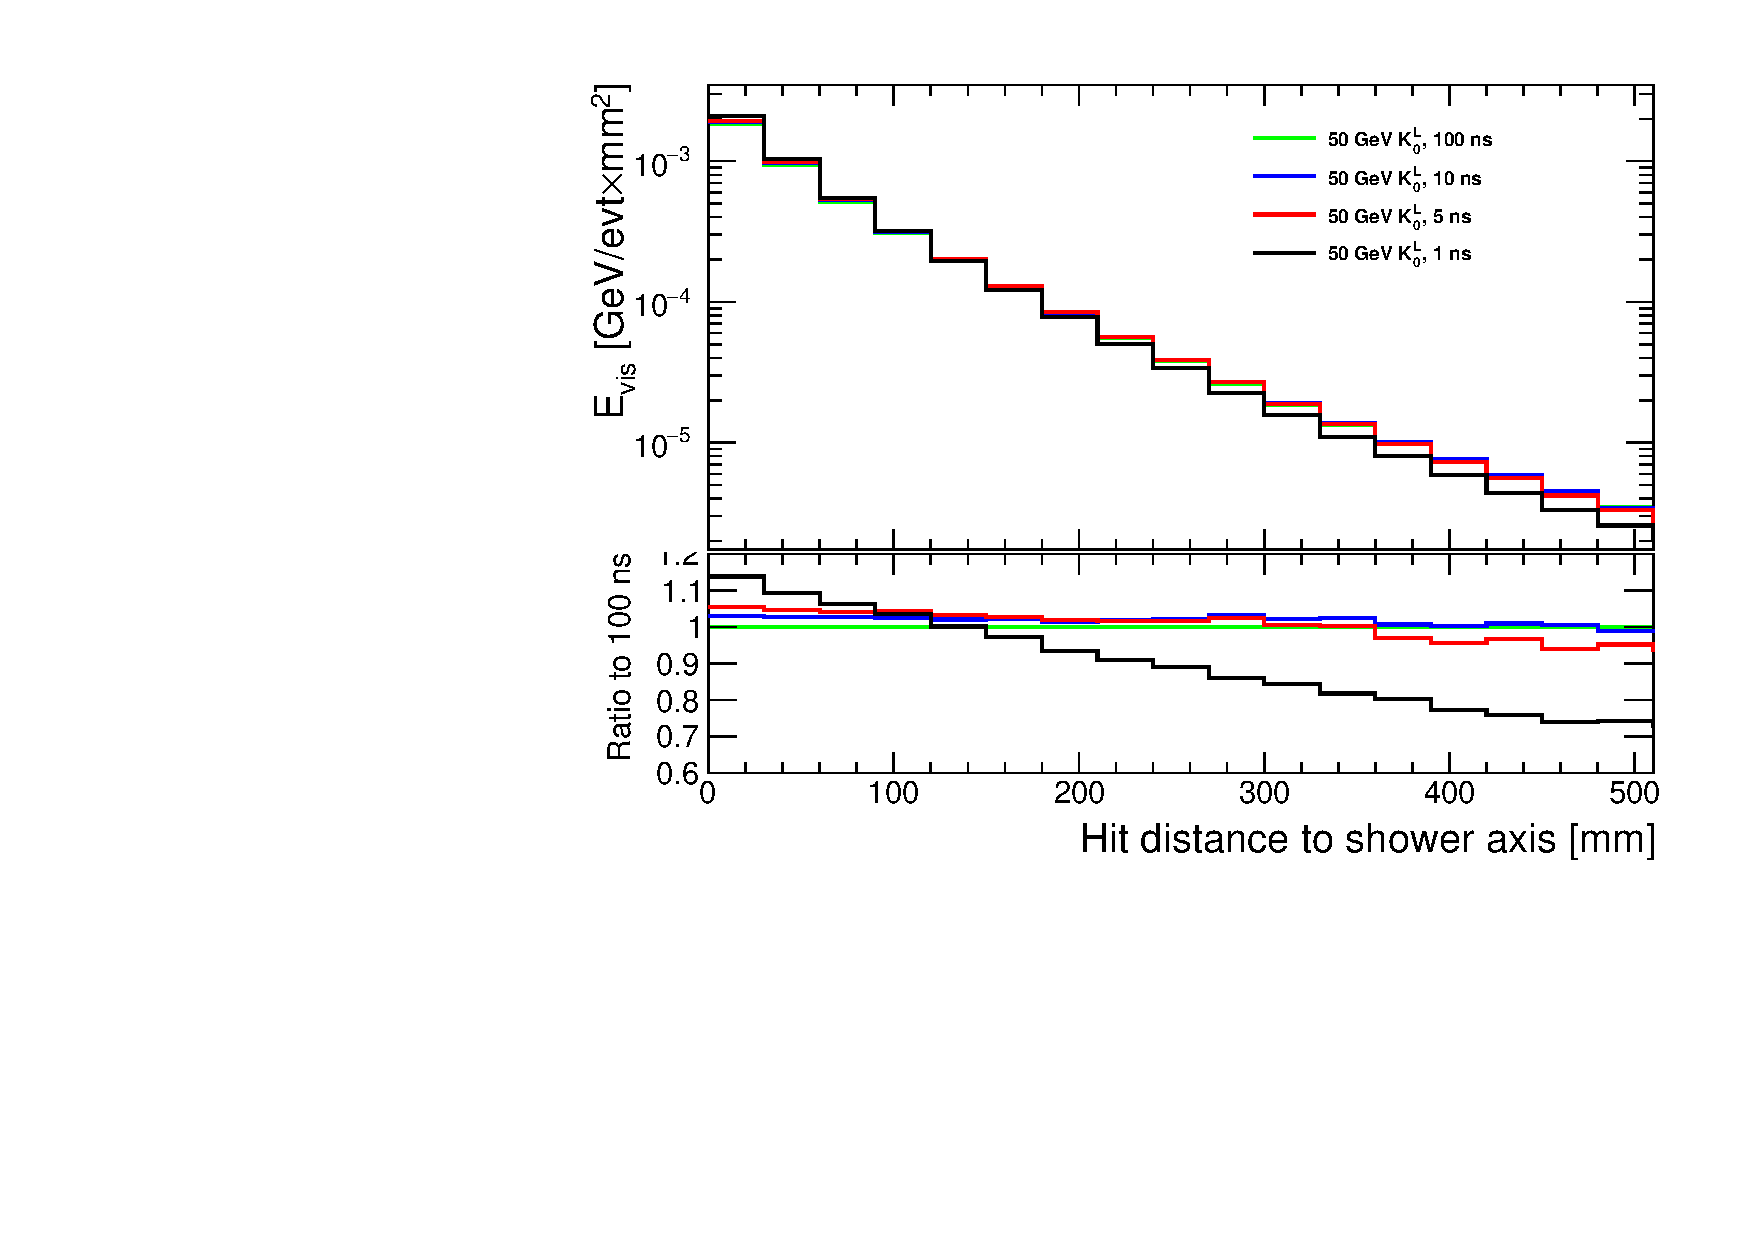
\includegraphics[width=0.7\linewidth]{../Thesis_Plots/ILD/NoSmearing/Plots/RadialProfileOverlay_noSmearing}
  \caption{The top plot shows the radial profile of a 50 \GeV hadronic shower overlaid for different timing cuts. The bottom plot shows the ratio of the histograms to \SI{100}{\nano\second} radial profile.} \label{fig:RadialProfNoSmearing}
\end{figure}

Another aspect looked at was the influence of timing cut on the shower width <R> (eq.\ref{eq:showerwidth}) defined as:

\begin{equation} \label{eq:showerwidth}
  <R> = \frac{\Sigma_i E_i r_i}{\Sigma_i E_i}
\end{equation}
\vspace{1ex}

The figures \ref{fig:ShowerWidthNoSmearing} and \ref{fig:ShowerWidthAbsoNoSmearing} show the shower width <R> for different particle energies as function of the timing cut. It shows that a tight timing cut at\SI{1}{\nano\second} can reduce the shower width up to around 70\%. One can observe also that the shower width at 5 and 10 \GeV are behaving differently than for higher energies. This may come from the transition from the Bertini model (BERT) to the quark string gluon model (QGSP) in the physics list in this energy range.

Looking at the shower width in absolute value, hadronic showers are slightly wider at lower energies ($\sim$\SI{125}{\milli\meter} for 10 GeV to $\sim$\SI{115}{\milli\meter} for 90 GeV) that may be related to the electromagnetic fraction in a hadronic shower that increases with energy thus reducing the shower width due to the energy weighting. Applying a timing cut removes more and more hits from the halo of the shower, thus reducing its size up to a point where it reaches the core of the shower at $\sim$\SI{20}{\nano\second} where the shower is around a couple of tiles in size. In general, all energies behave in a rather similar manner.

\begin{figure}[htbp!]
  \centering
  \begin{subfigure}[t]{0.49\textwidth}
    \centering
    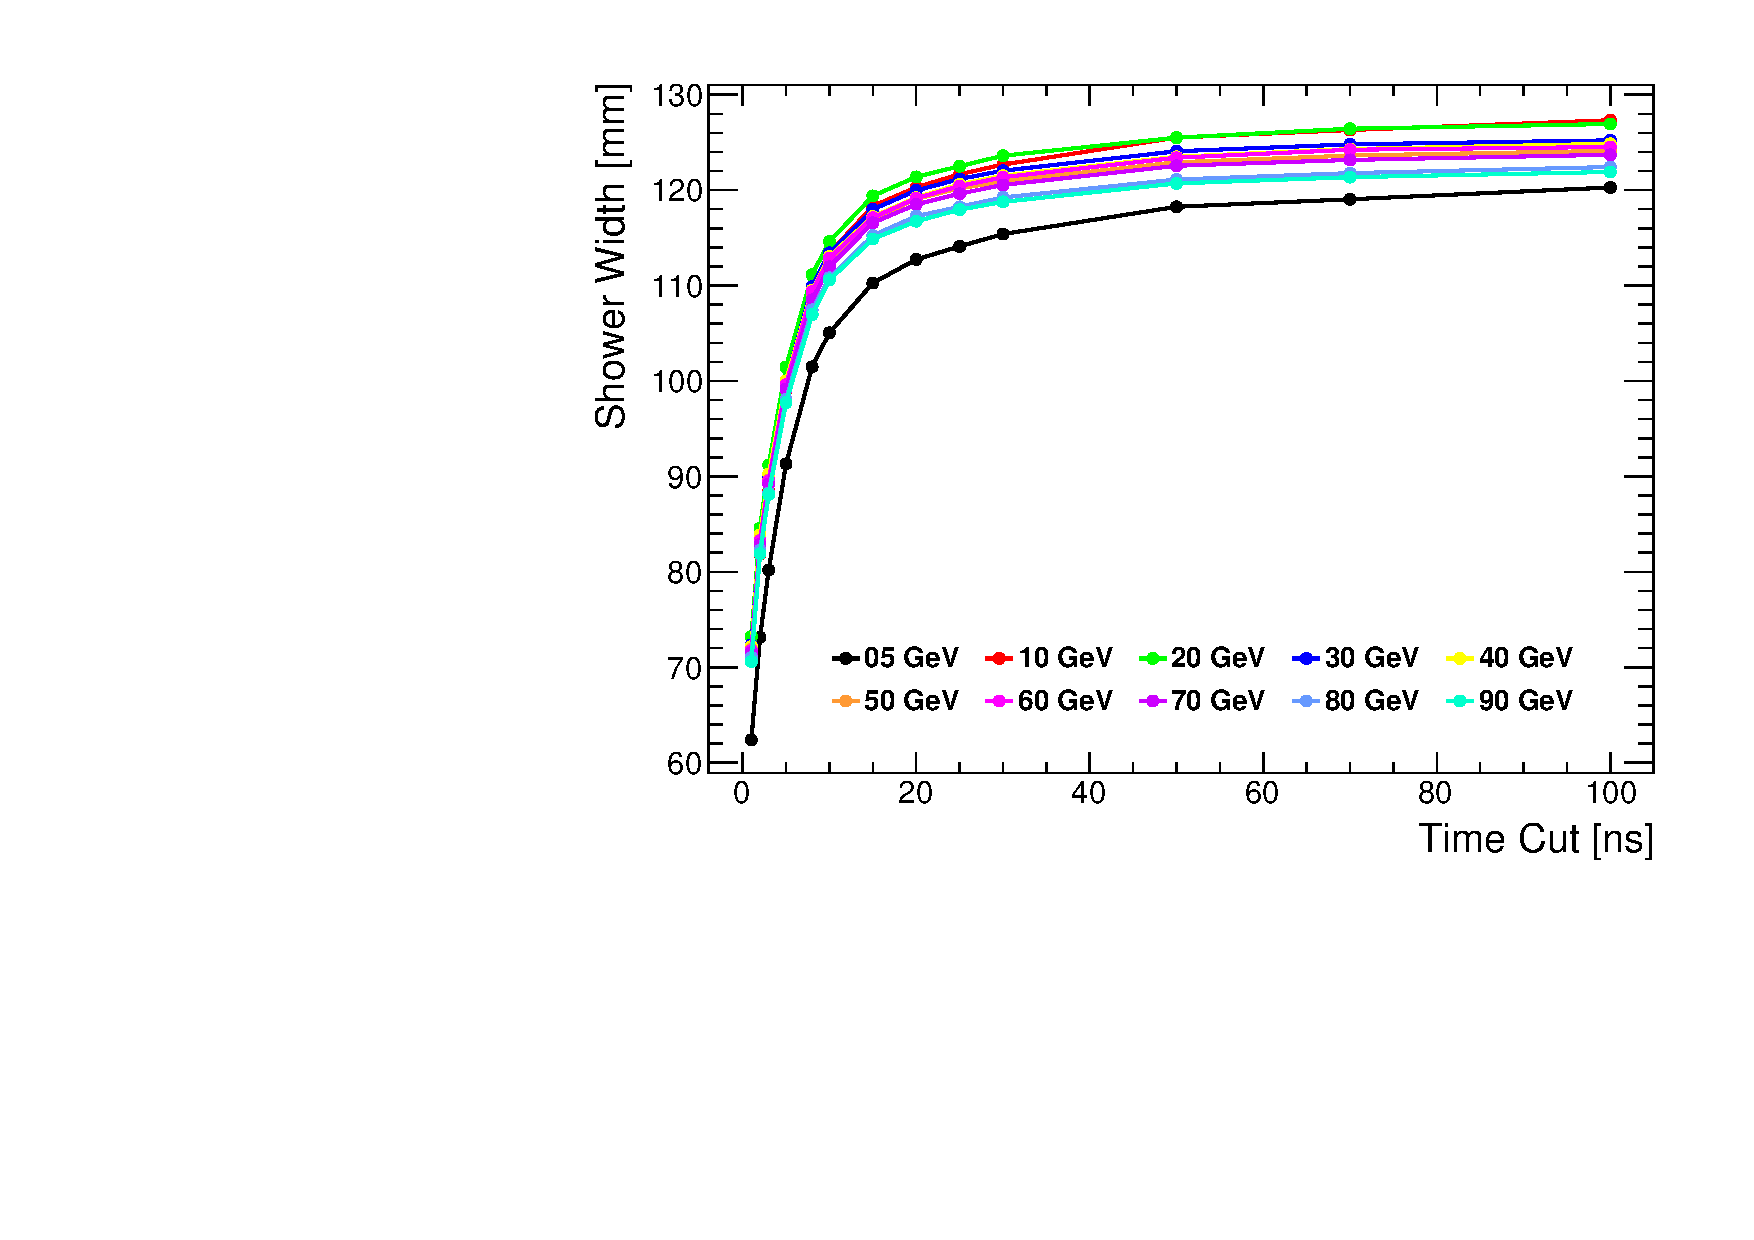
\includegraphics[width=1\linewidth]{../Thesis_Plots/ILD/NoSmearing/Plots/ShowerWidthAbso_TimeCuts_noSmearing}
    \caption{} \label{fig:ShowerWidthAbsoNoSmearing}
  \end{subfigure}
  \begin{subfigure}[t]{0.49\textwidth}
    \centering
    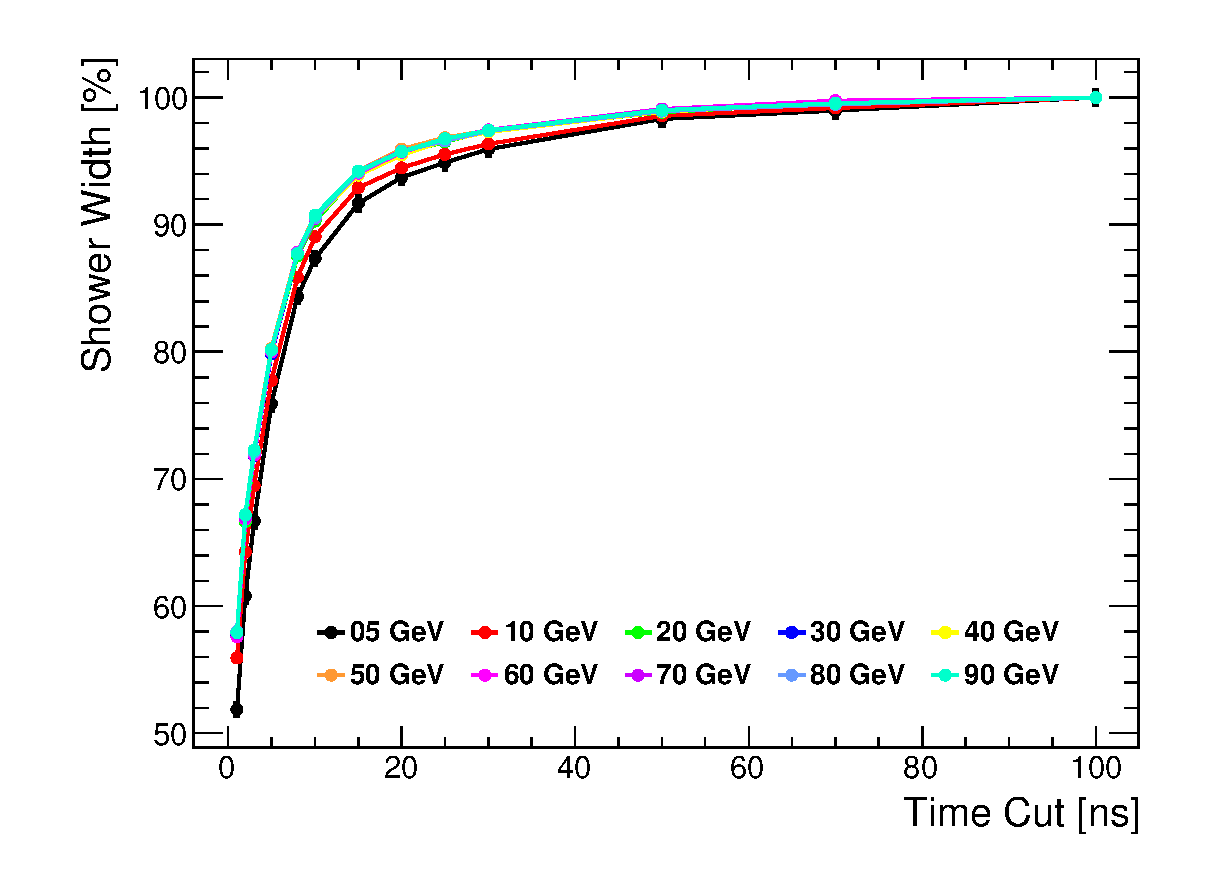
\includegraphics[width=1\linewidth]{../Thesis_Plots/ILD/NoSmearing/Plots/ShowerWidth_TimeCuts_noSmearing}
    \caption{} \label{fig:ShowerWidthNoSmearing}
  \end{subfigure}
  \caption{\subref{fig:ShowerWidthAbsoNoSmearing}) The plots represents the absolute value of the mean shower width <R> in \SI{}{\milli\meter} as function of the timing cut. This shows that the low energy showers are generally wider certainly due to the magnetic field. And under \SI{20}{\nano\second}, the width is very similar indicating the core of the shower is fairly similar for all energies. \subref{fig:ShowerWidthNoSmearing}) The plot represents the mean of the shower width <R> as function of timing cut for different particle energies. The y-axis has been normalized to the shower width at \SI{100}{\nano\second}. The shower width decreases steadily as function of the timing cut, indicating that the shower gets narrower.}
\end{figure}

\begin{figure}[htbp!]
  \centering
  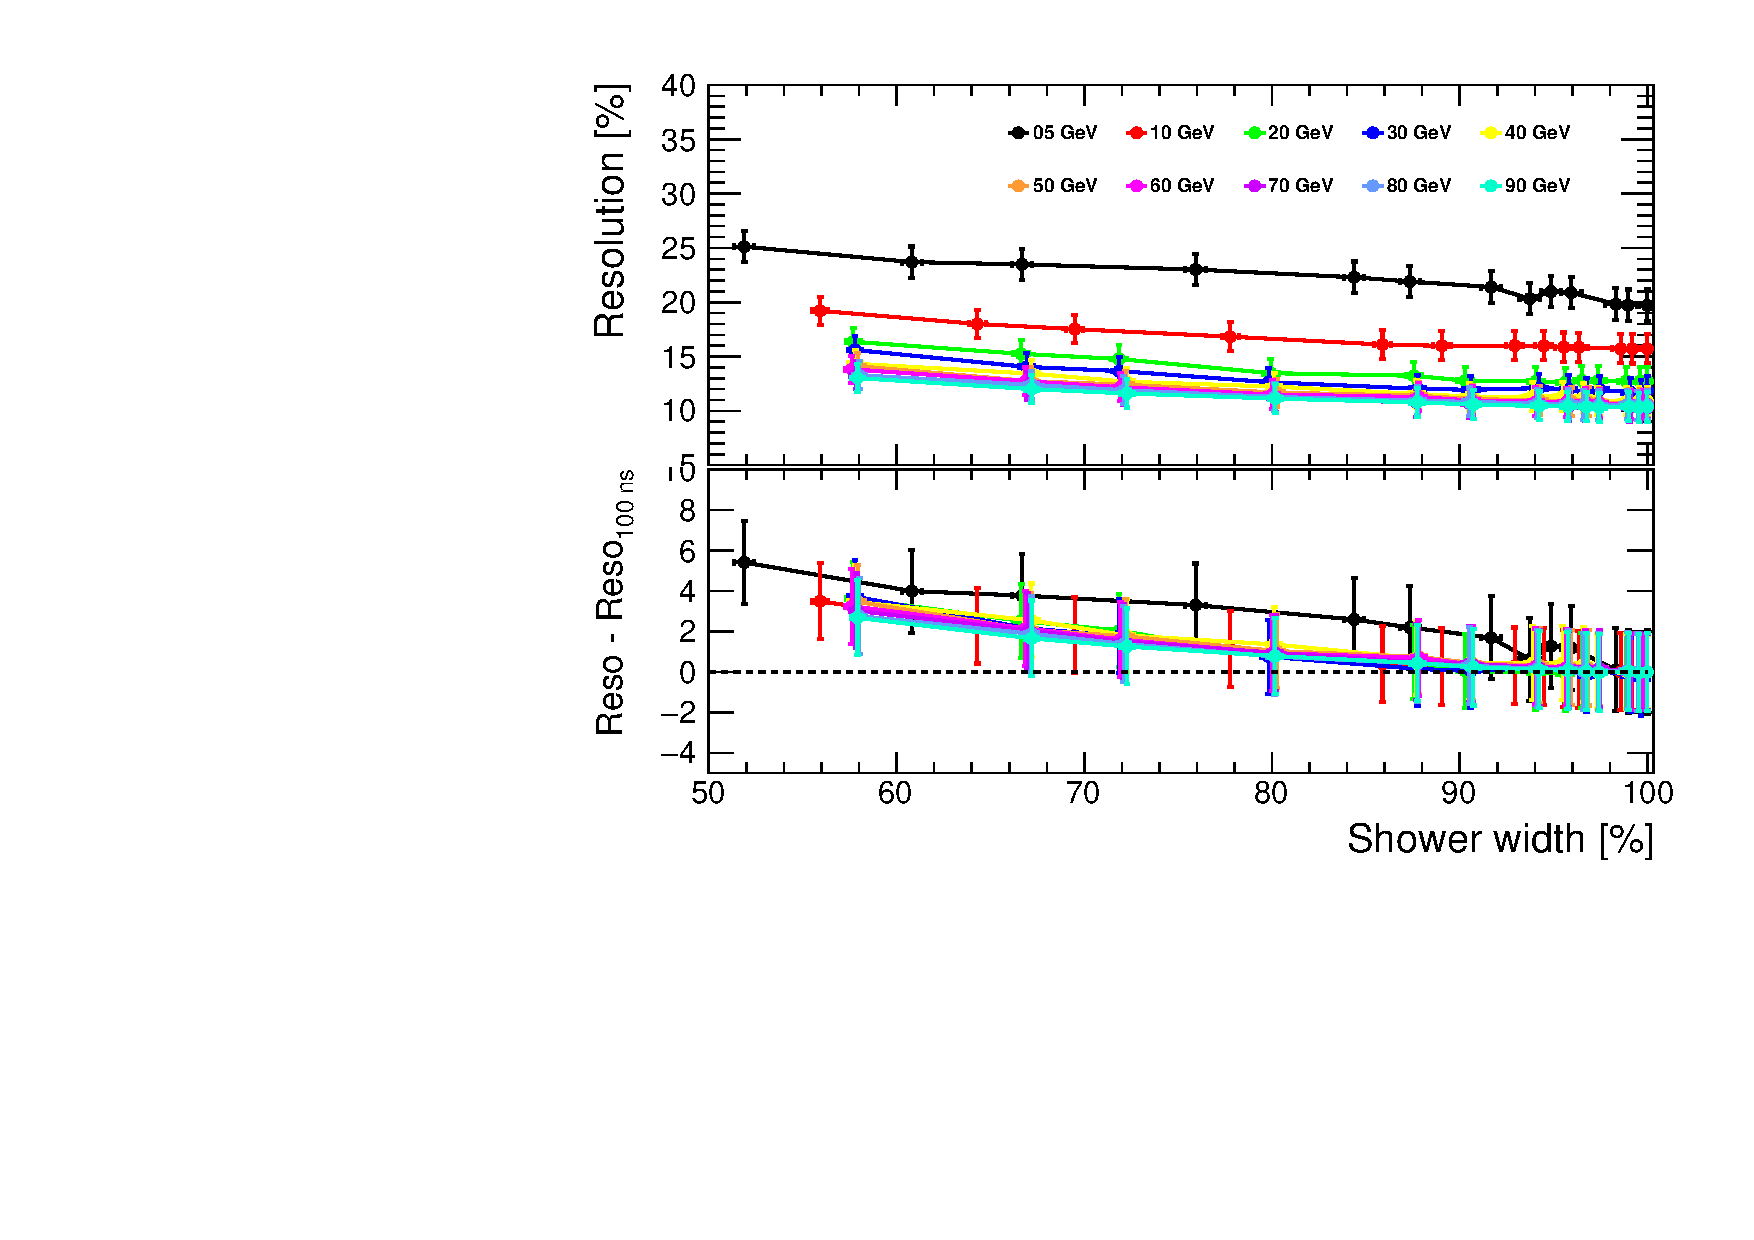
\includegraphics[width=0.7\linewidth]{../Thesis_Plots/ILD/NoSmearing/Plots/ShowerWidth_Resolution_noSmearing}
  \caption{The top plot is the energy resolution as function of shower width for different particle energies. Each point represents a timing cut from \SI{1}{\nano\second} ns to \SI{100}{\nano\second} from left to right. The bottom plot is the loss of resolution compared to the reduction in shower width size.} \label{fig:ShowerWidthResoNoSmearing}
\end{figure}

It is interesting to look at the gain in the reduction of the shower width compared to the loss in energy resolution. In fact, reducing the shower width could help to improve the pattern recognition in Pandora. The figure \ref{fig:ShowerWidthResoNoSmearing} shows the resolution loss as function of the shower width. The bottom plots show the gain in shower width is behaving in the same way for all energies. The tighter the timing cut gets, the small the shower gets as well as a loss in resolution. The main point here is that the gain in shower width is great (up to 40\% decrease in width) compared to the loss in energy resolution (around 4-6\%) that could be recovered in a next step after pattern recognition.

This study shows that the use of timing cuts give a great advantage in order to improve pattern recognition without degrading too much the energy resolution of a hadronic shower. However, this study assumes a perfect timing resolution which does not reflect the reality. In the next section, different time resolutions were assumed based on the current knowledge on the timing resolution of the foreseen electronics.

\subsection{In a realistic scenario}

In this section, a similar study is performed as in previous section \ref{sec:MCLevelILDTiming}. Instead, it assumes realistic time resolutions based on the current electronic technology. The table \ref{table:TimeReso} sums up the investigated time resolutions. The same selection is applied as in the previous section.

% \begin{figure}[htbp!]
%   \centering
%   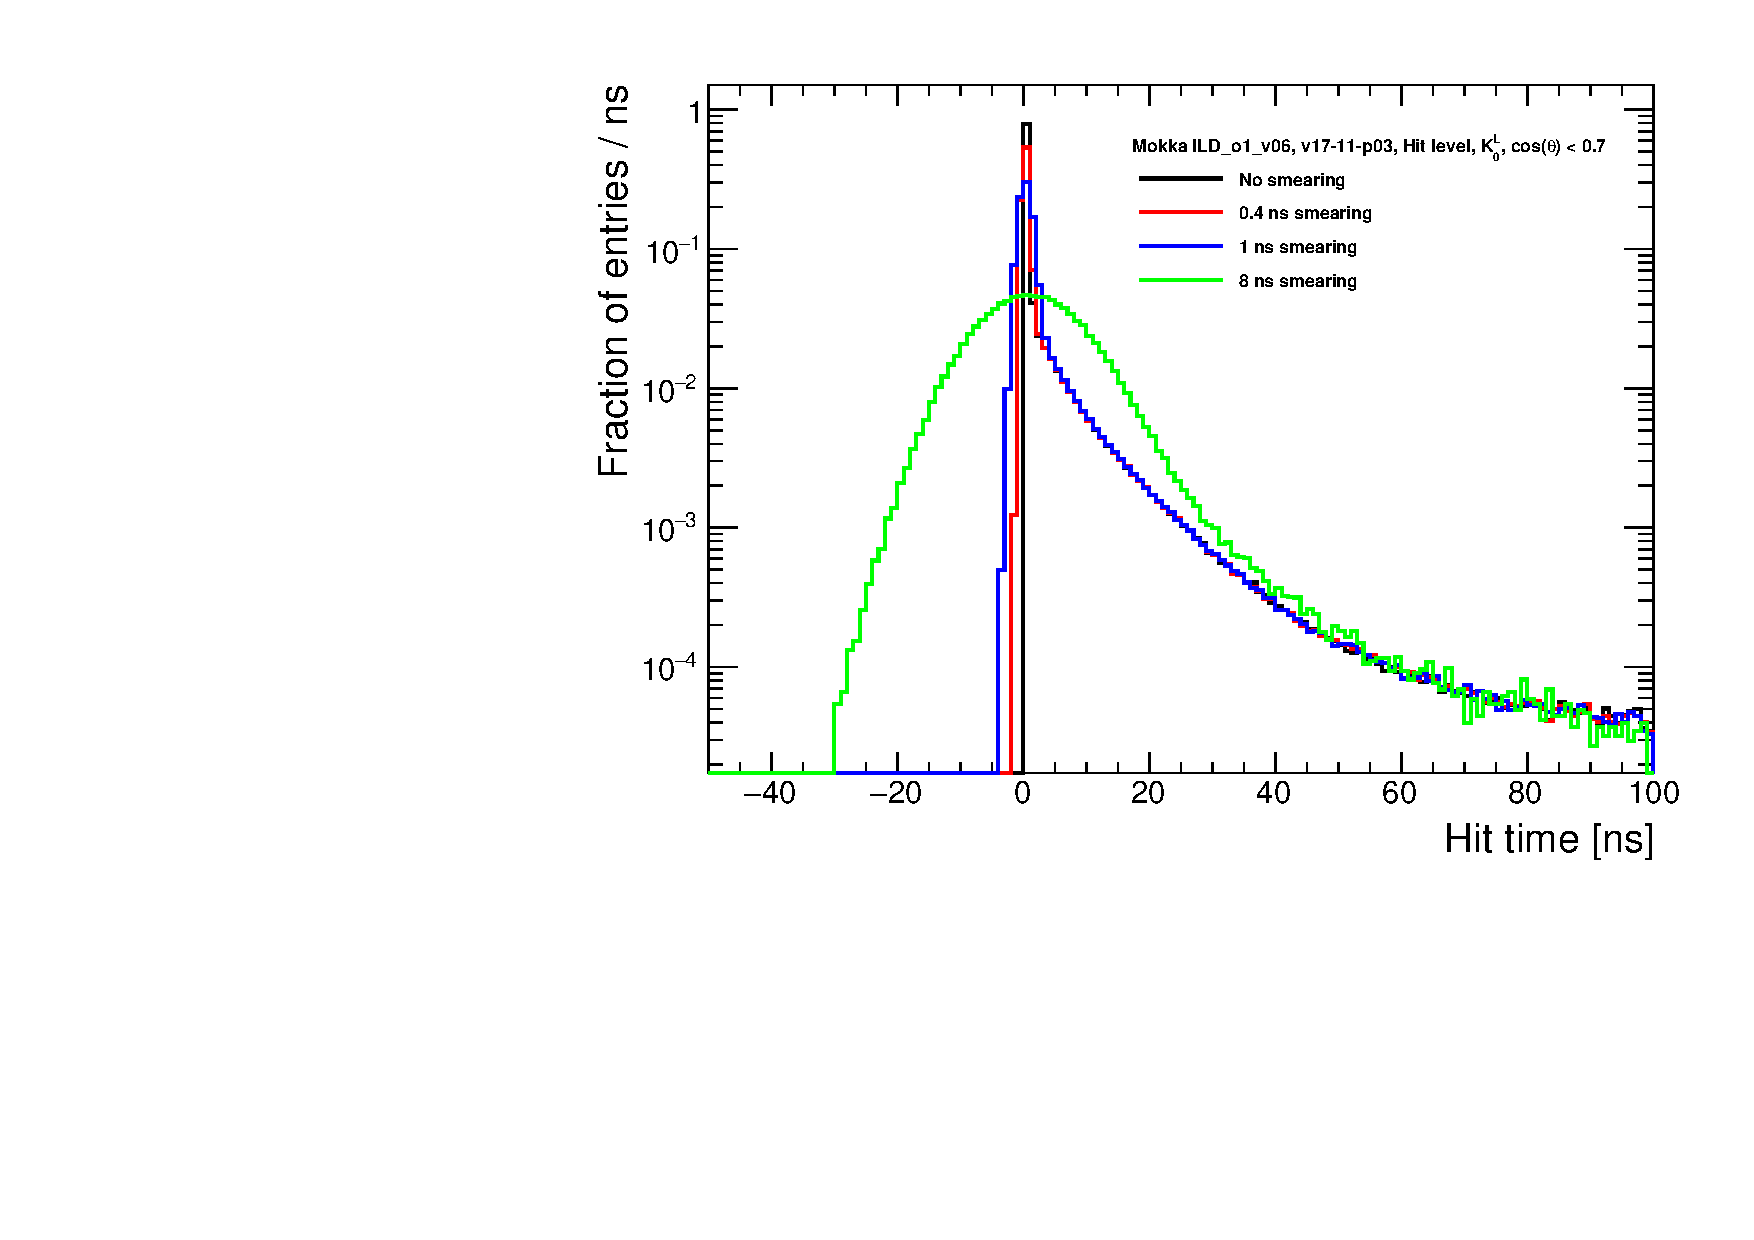
\includegraphics[width=0.7\linewidth]{../Thesis_Plots/ILD/TimeDistribution/Plots/ComparisonSmearingTimingAHCAL}
%   \caption{Distribution of the time of all hits in the AHCAL with different values used for time smearing.} \label{fig:SmearingAHCAL}
% \end{figure}

\begin{table}[htb!]
  \centering
  \caption{Time resolution used for smearing.} \label{table:TimeReso}
  \begin{tabular}{|c|c|}
    \hline
    Scenario & Time resolution (ns) \\
    \hline
    Testbeam & 8 \\
    Ideal & 1 \\
    ILC extrapolated & 0.4 \\
    \hline
  \end{tabular}
\end{table}

The testbeam resolution is the time resolution obtained with the current AHCAL technological prototype as shown in section \ref{subsec:Electron_Final}. The ideal time resolution is in the order of the timescale of the development of hadronic showers. And finally, the ILC extrapolated time resolution is obtained by assuming a linear extrapolation from the testbeam time resolution with a faster slow clock of \SI{5}{\mega\hertz} instead of \SI{250}{\kilo\hertz} (x20 faster) as explained in section \ref{subsec:SPIROC2B}, though this is probably optimistic.

\begin{figure}[htbp!]
  \centering
  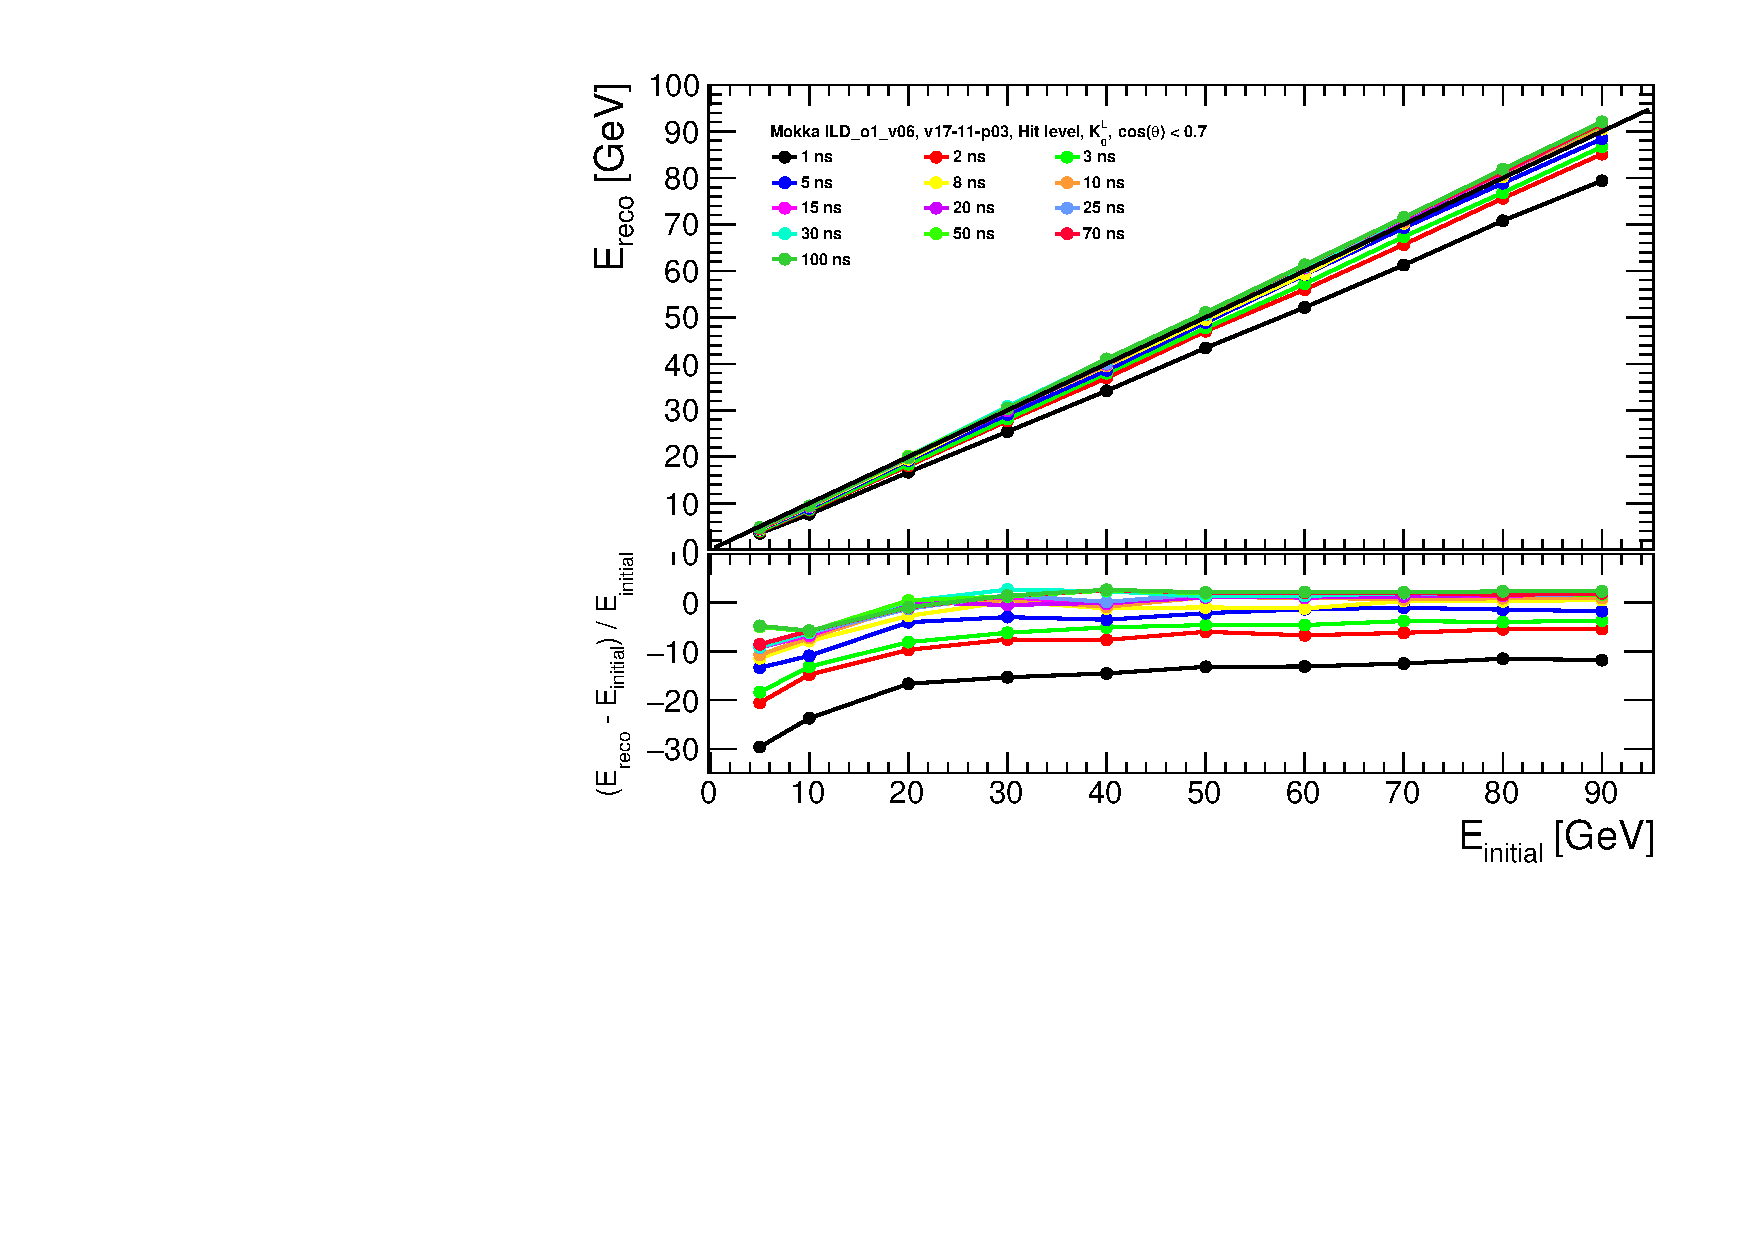
\includegraphics[width=0.7\linewidth]{../Thesis_Plots/ILD/Smearing_0.4ns/Plots/Linearity_TimeCuts_Smearing1}
  \caption{Linearity curves for \SI{0.4}{\nano\second} time resolution. The top plot represents the mean reconstructed energy $E_{reco}$ for kaons from 5 to 90 \GeV. The bottom plot shows the relative deviation to the line $x=y$.} \label{fig:Lin0.4ns}
\end{figure}

\begin{figure}[htbp!]
  \centering
  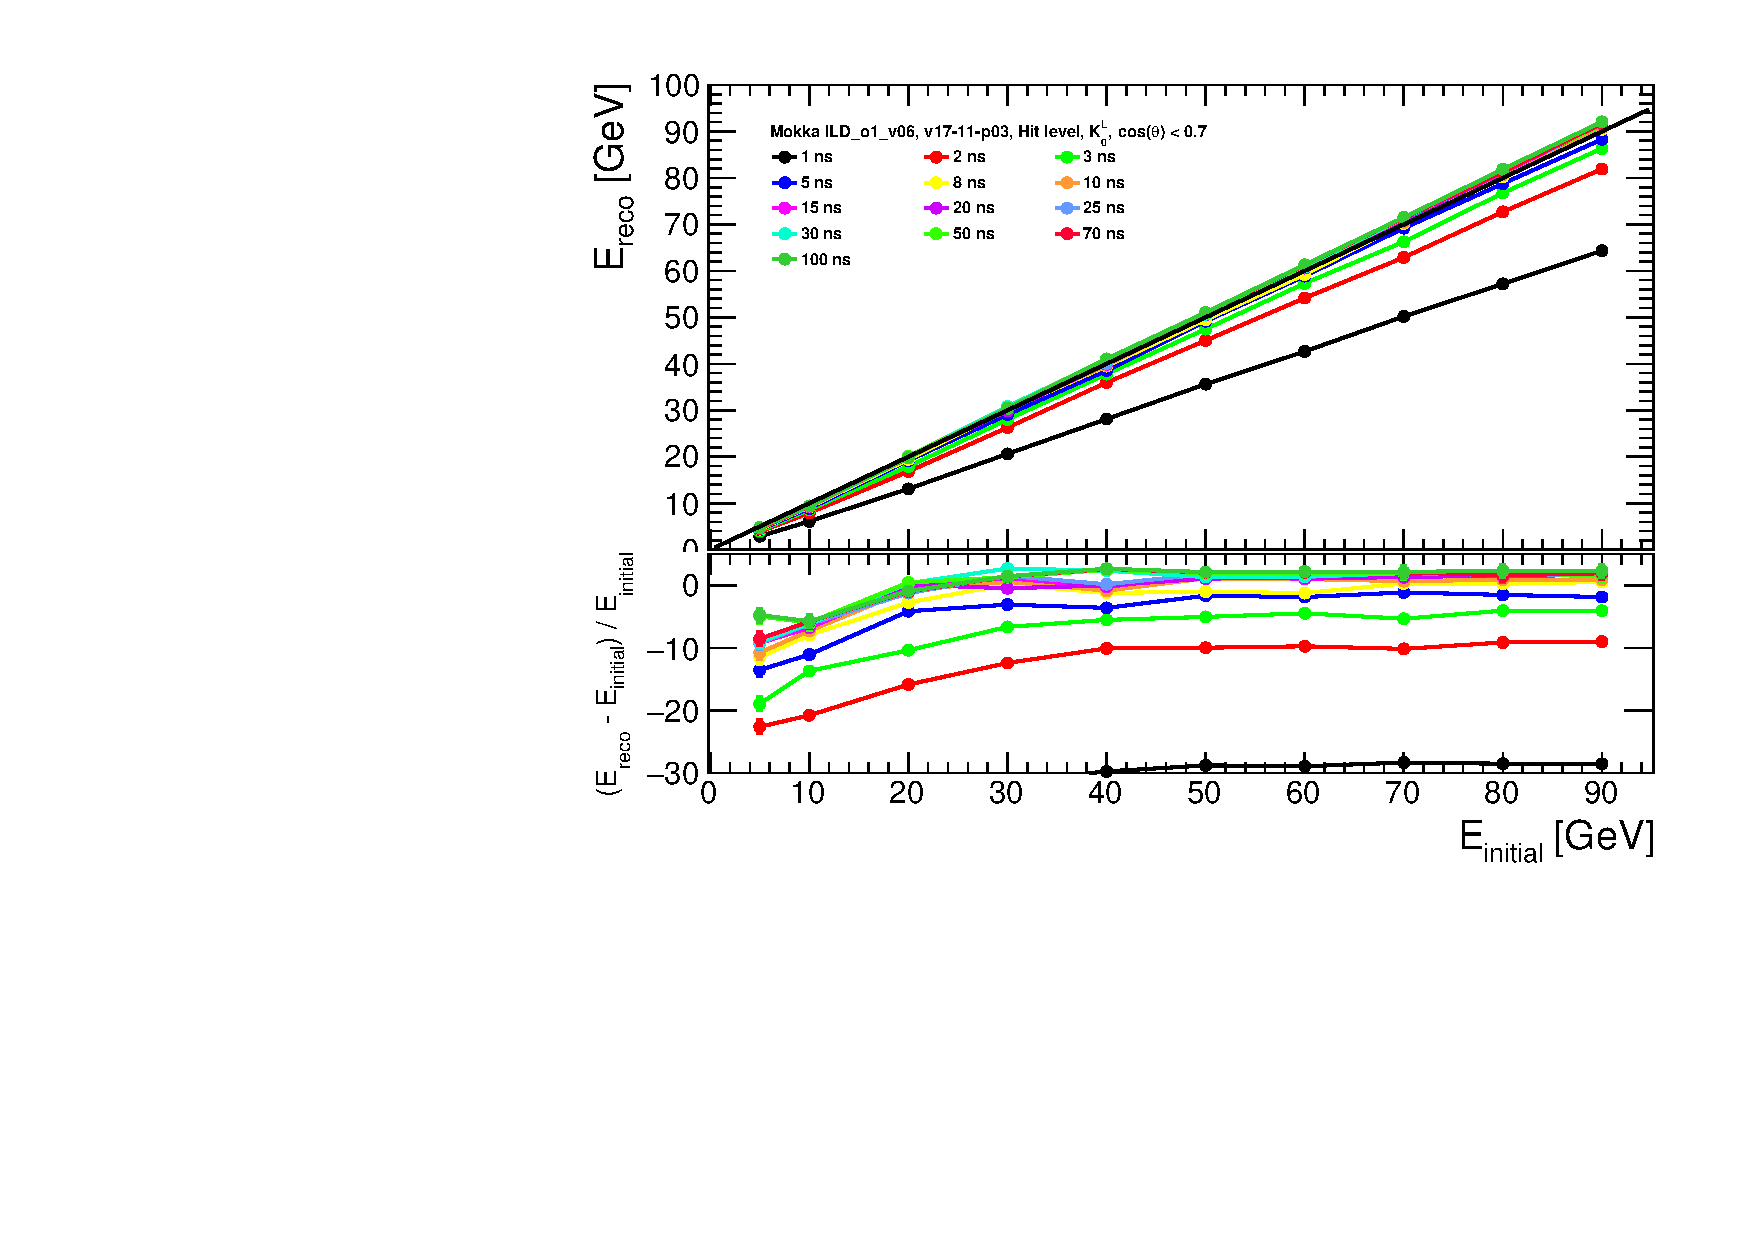
\includegraphics[width=0.7\linewidth]{../Thesis_Plots/ILD/Smearing_1ns/Plots/Linearity_TimeCuts_Smearing2}
  \caption{Linearity curves \SI{1}{\nano\second} time resolution. The top plot represents the mean reconstructed energy $E_{reco}$ for kaons from 5 to 90 \GeV. The bottom plot shows the relative deviation to the line $x=y$.} \label{fig:Lin1ns}
\end{figure}

\begin{figure}[htbp!]
  \centering
  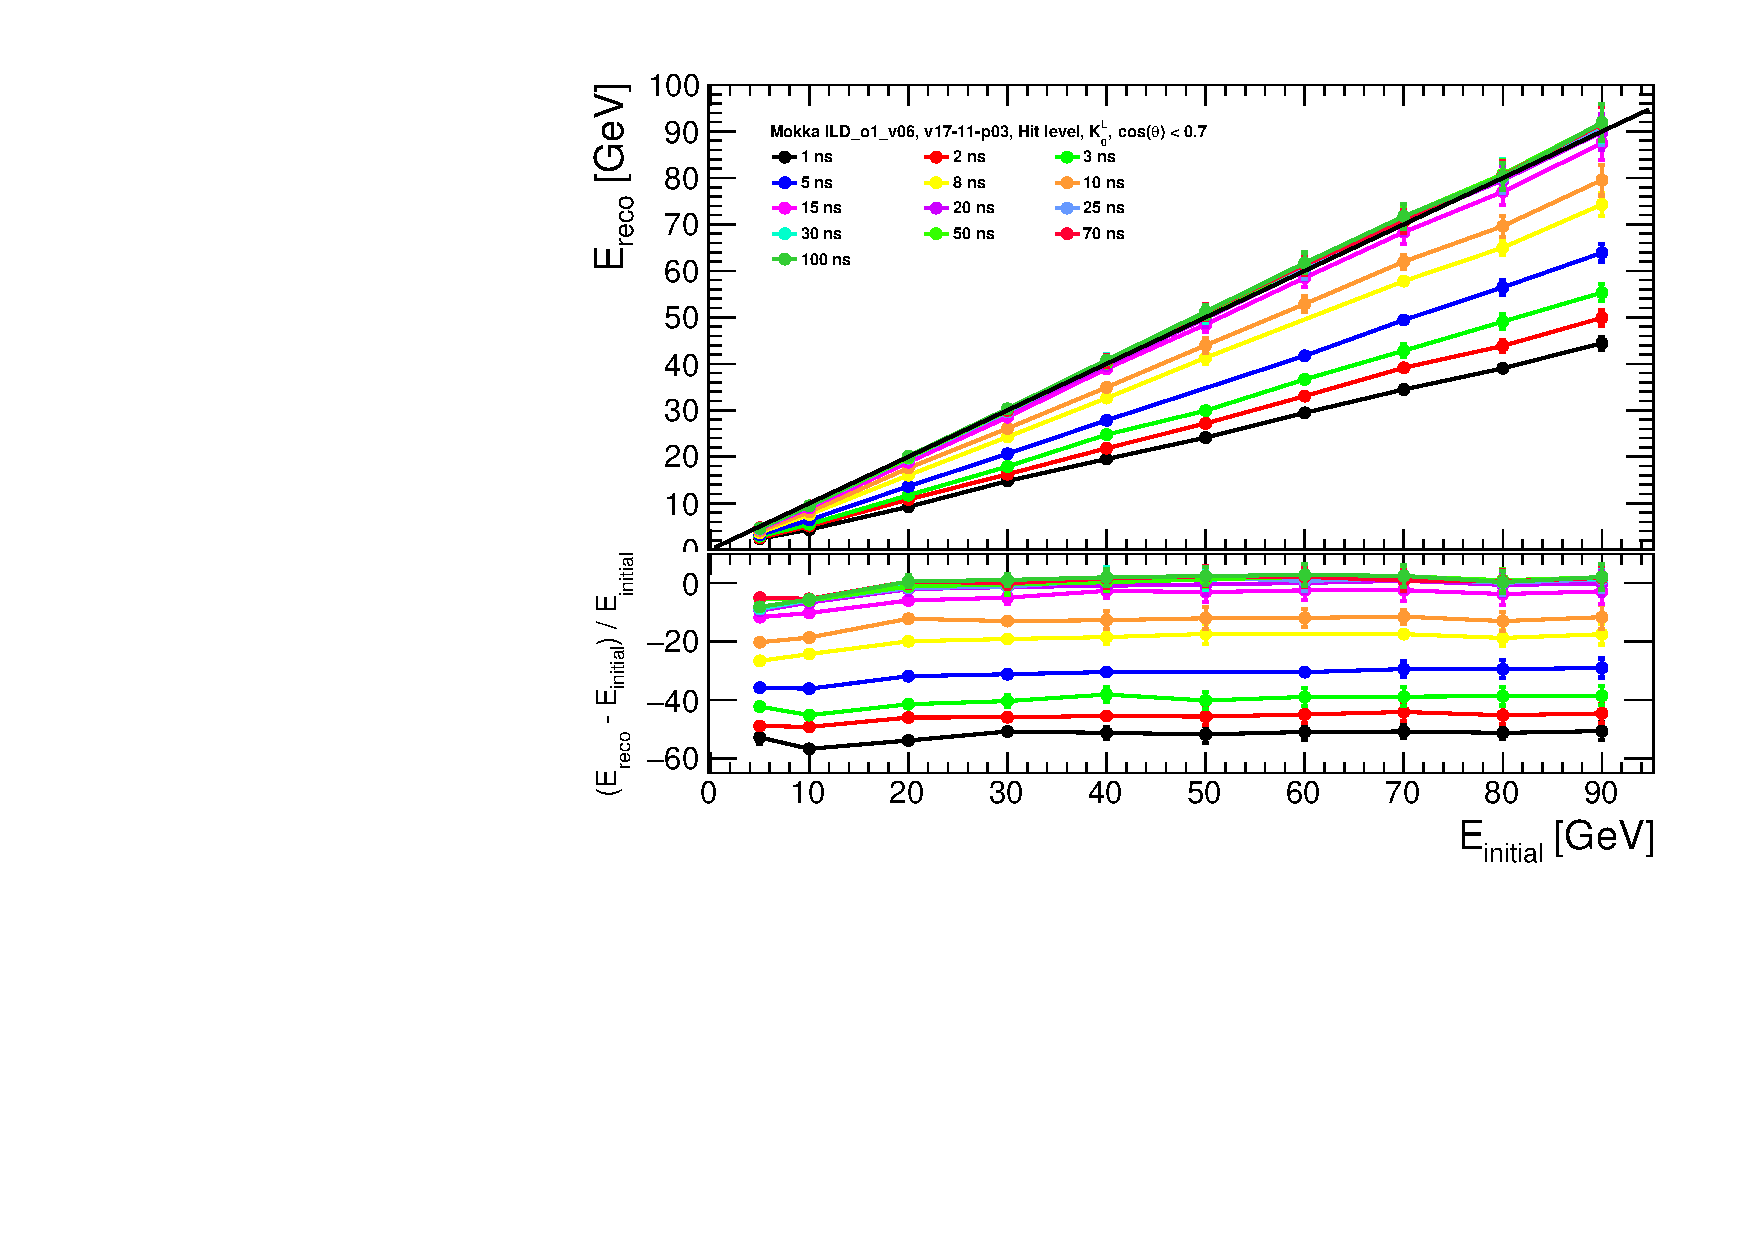
\includegraphics[width=0.7\linewidth]{../Thesis_Plots/ILD/Smearing_8ns/Plots/Linearity_TimeCuts_Smearing3}
  \caption{Linearity curves \SI{8}{\nano\second} time resolution. The top plot represents the mean reconstructed energy $E_{reco}$ for kaons from 5 to 90 \GeV. The bottom plot shows the relative deviation to the line $x=y$.}  \label{fig:Lin8ns}
\end{figure}

Looking at the impact on linearity and energy resolution, time resolution in the order of sub-nanosecond does not affect much the linearity and resolution as shown in figures \ref{fig:Lin0.4ns} and \ref{fig:Reso0.4ns}. For a time resolution in the nanosecond order, the linearity and resolution does not get affected much as shown in figures \ref{fig:Lin1ns} and \ref{fig:Reso1ns}. Of course, for a cut below 1-2 ns, it will start to degrade the linearity rapidly, between 35-40\% for 1 ns time resolution. The resolution gets affected as well, by around 35-50\%. For the 8 ns timing resolution, the linearity and resolution, as shown in figures \ref{fig:Lin8ns} and \ref{fig:Reso8ns}, start to get heavily degraded for timing cuts below 10-20 \SI{}{\nano\second}, around 55-60\% for the linearity and around 50-60\% for the resolution.

\begin{figure}[htbp!]
  \centering
  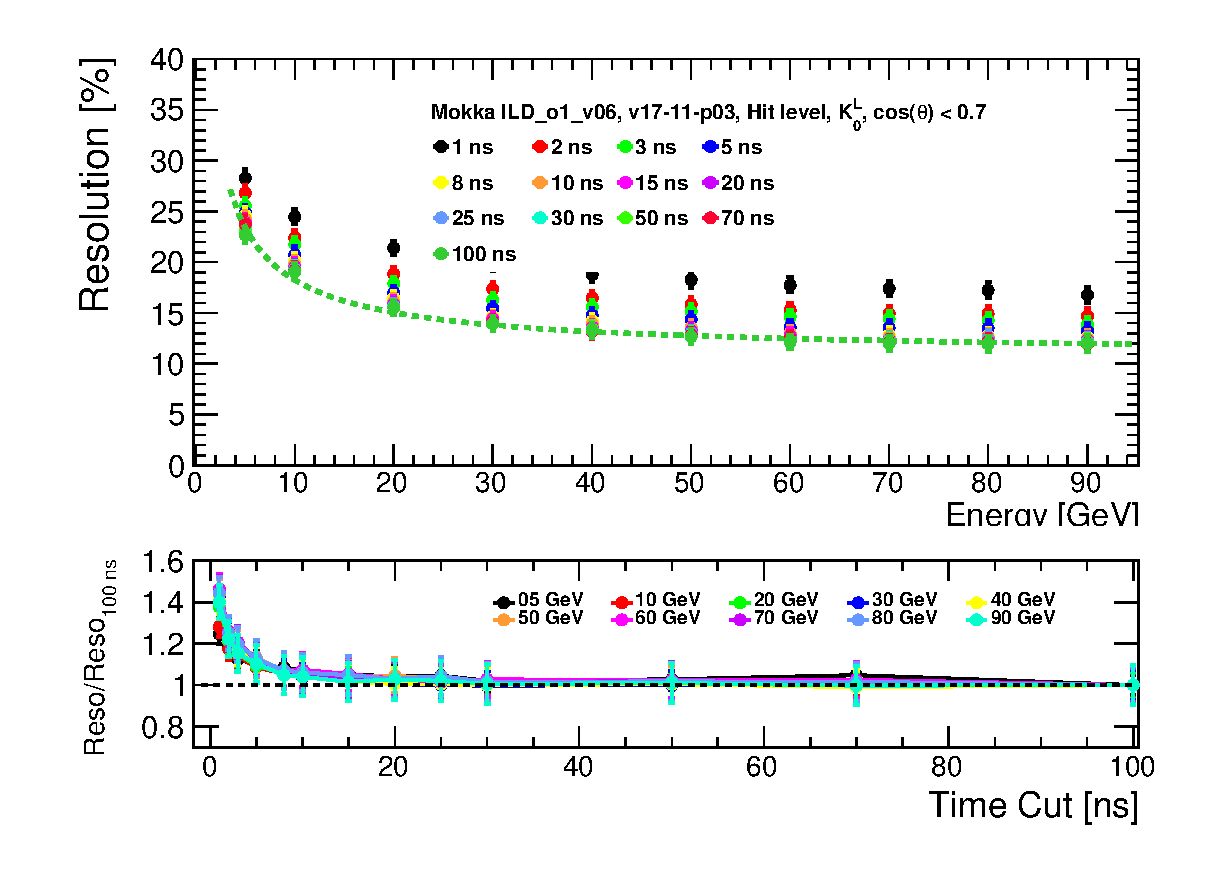
\includegraphics[width=0.7\linewidth]{../Thesis_Plots/ILD/Smearing_0.4ns/Plots/ShowerResoAbsolute_TimeCuts_Smearing1}
  \caption{Energy resolution curves for \SI{0.4}{\nano\second} time resolution. The plot represents the relative energy resolution $\frac{\sigma_{E}}{E}$ for kaons from 5 to 90 \GeV for each timing cut. The green line is a fit applied to 100 ns timing cut of the typical form $\frac{\sigma_{E}}{E} = \frac{a}{\sqrt{E}} \bigoplus b$.} \label{fig:Reso0.4ns}
\end{figure}

\begin{figure}[htbp!]
  \centering
  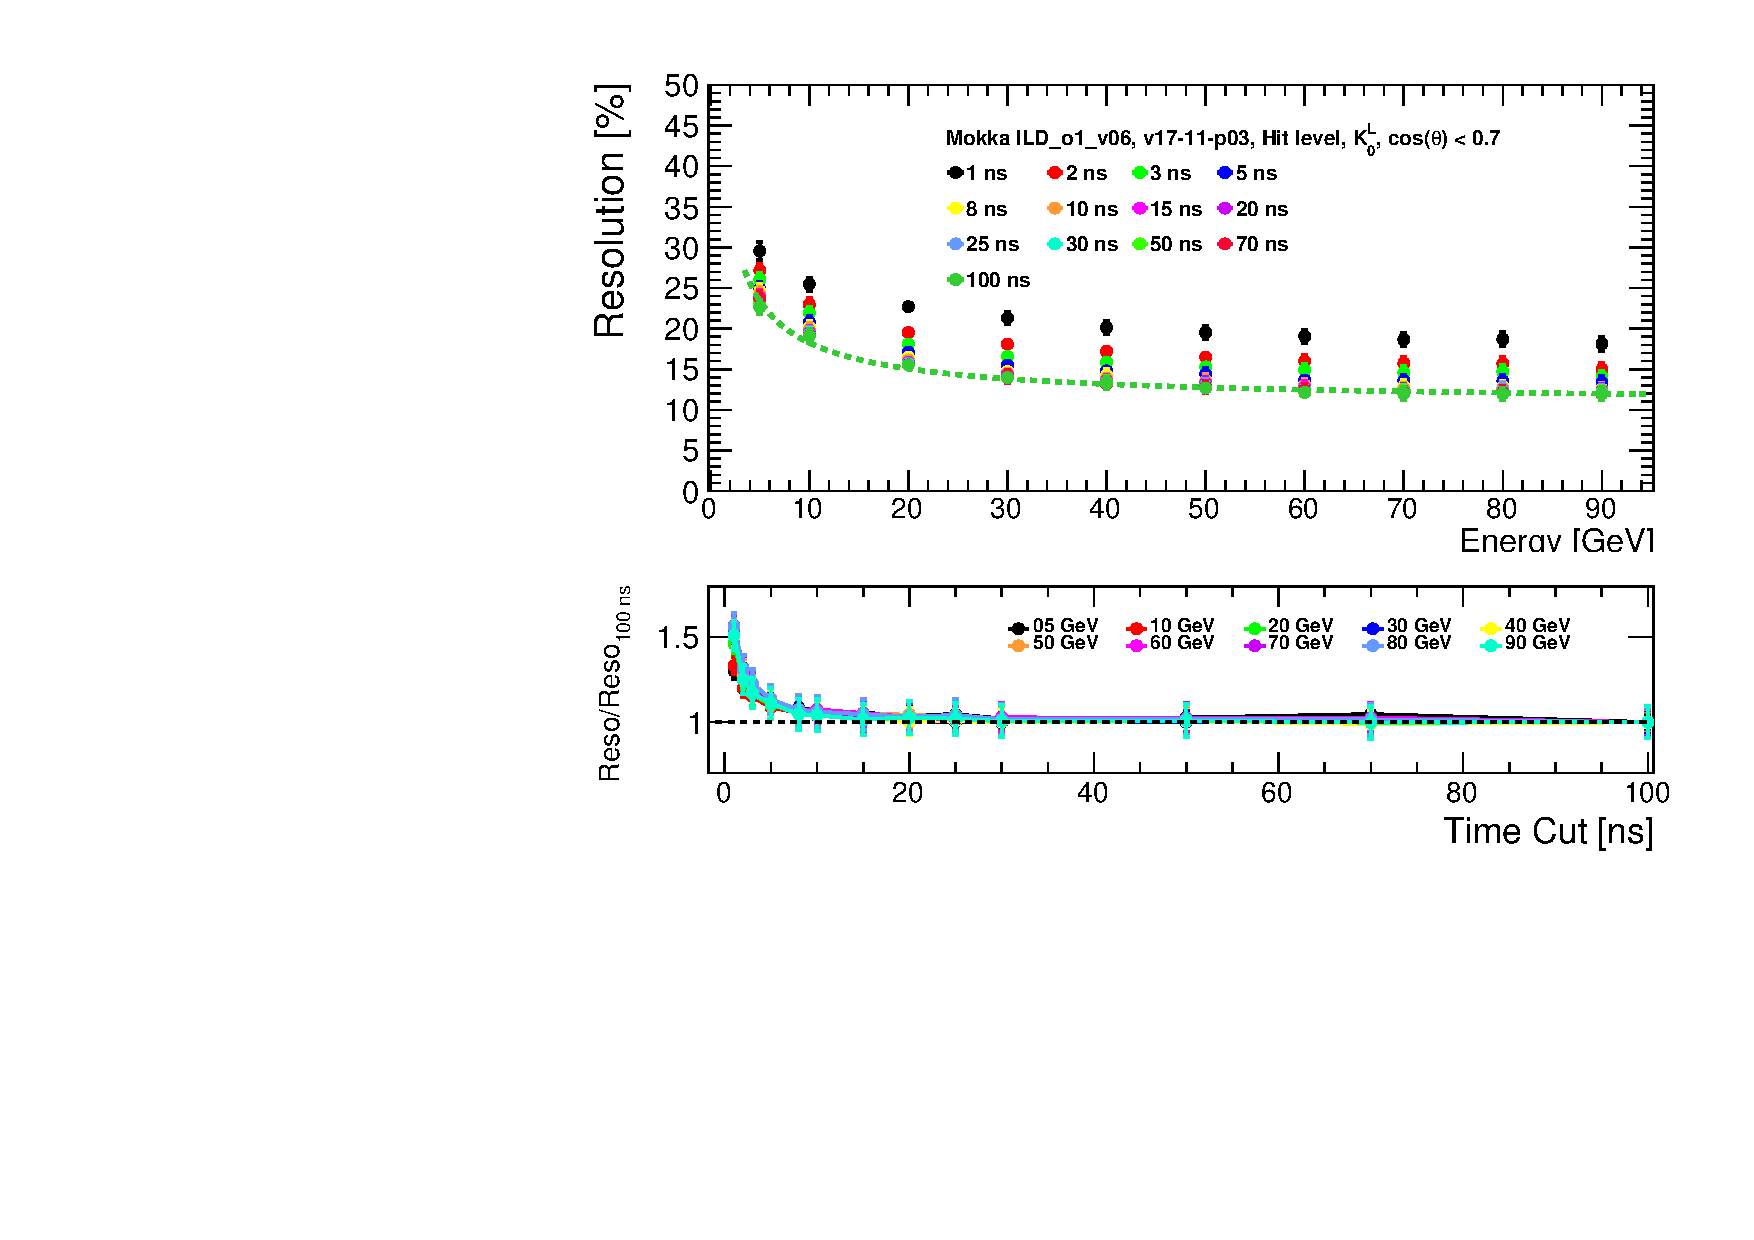
\includegraphics[width=0.7\linewidth]{../Thesis_Plots/ILD/Smearing_1ns/Plots/ShowerResoAbsolute_TimeCuts_Smearing2}
  \caption{Energy resolution curves for \SI{1}{\nano\second} time resolution. The plot represents the relative energy resolution $\frac{\sigma_{E}}{E}$ for kaons from 5 to 90 \GeV for each timing cut. The green line is a fit applied to 100 ns timing cut of the typical form $\frac{\sigma_{E}}{E} = \frac{a}{\sqrt{E}} \bigoplus b$.} \label{fig:Reso1ns}
\end{figure}

\begin{figure}[htbp!]
  \centering
  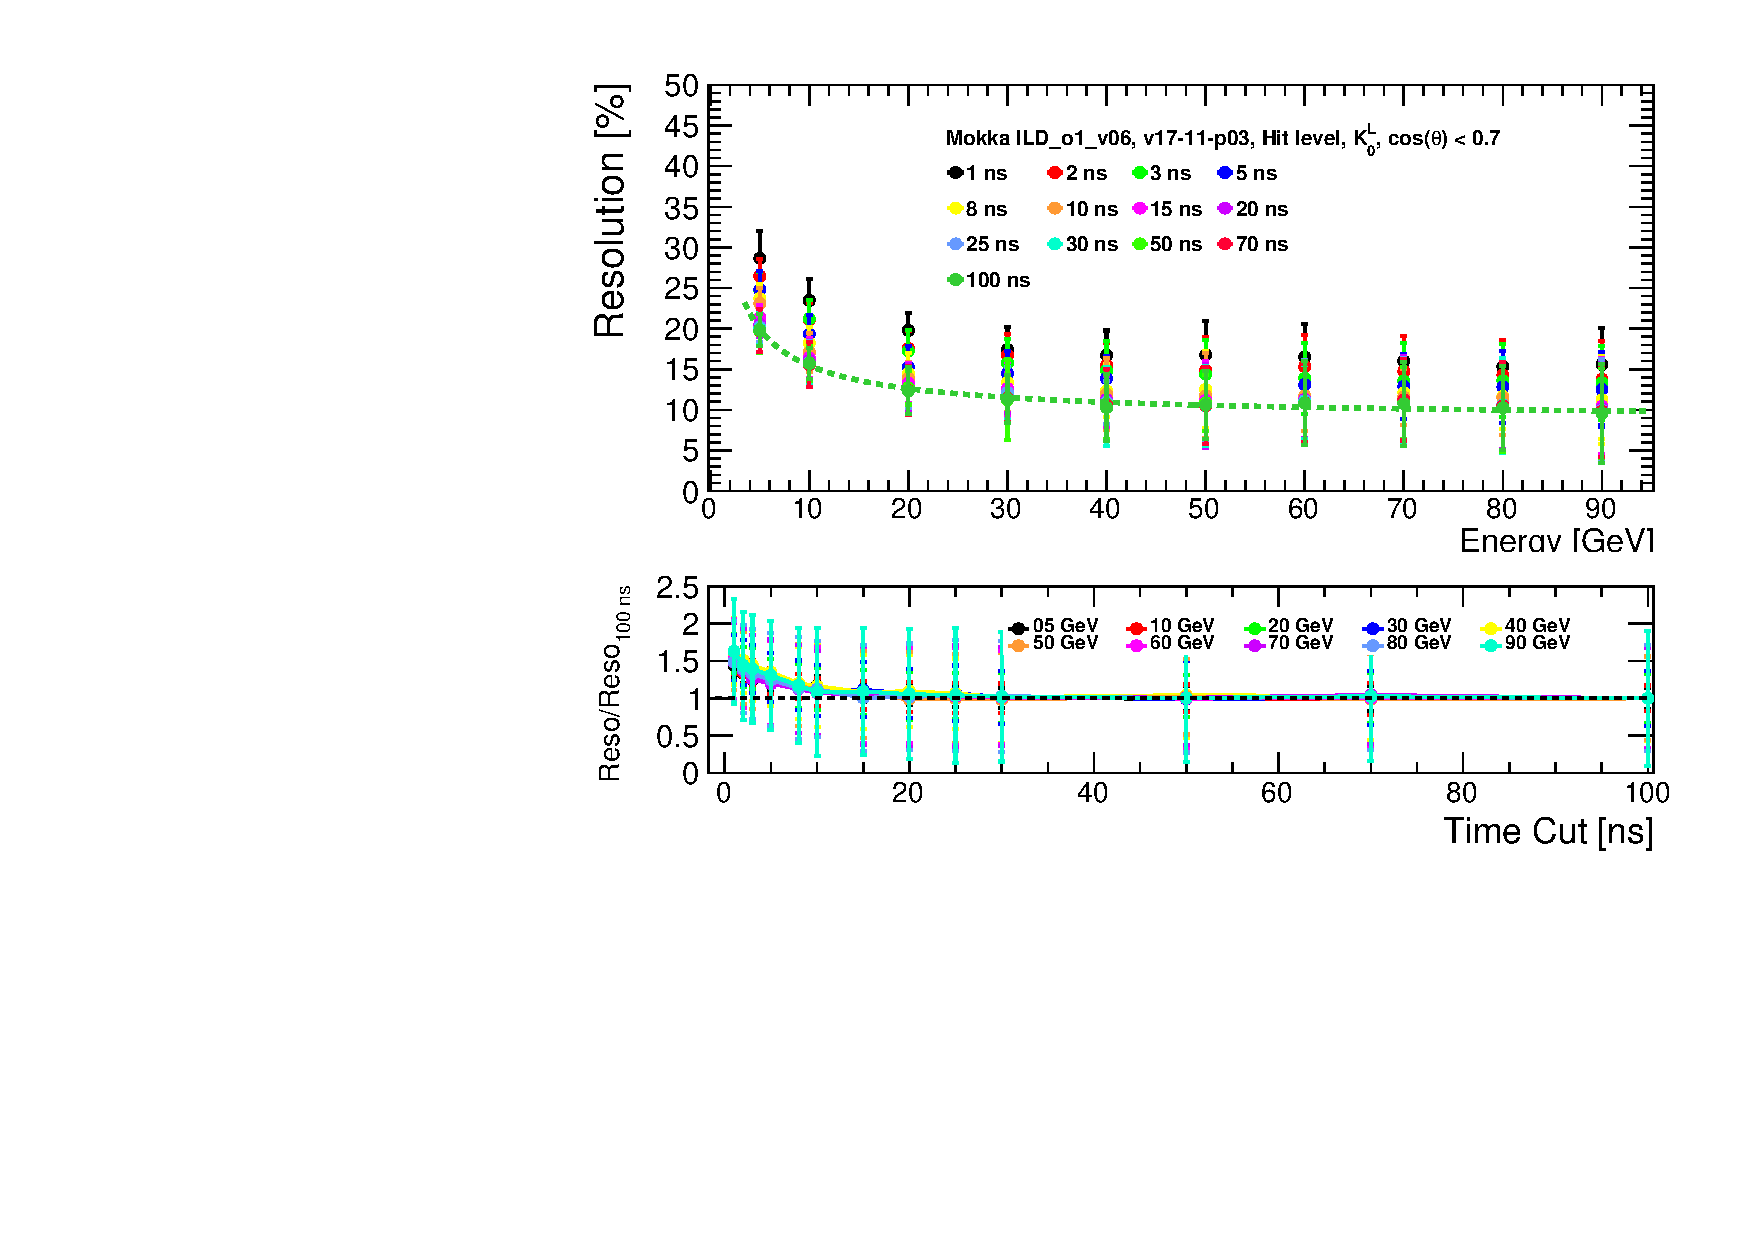
\includegraphics[width=0.7\linewidth]{../Thesis_Plots/ILD/Smearing_8ns/Plots/ShowerResoAbsolute_TimeCuts_Smearing3}
  \caption{Energy resolution curves for \SI{8}{\nano\second} time resolution. The plot represents the relative energy resolution $\frac{\sigma_{E}}{E}$ for kaons from 5 to 90 \GeV for each timing cut. The green line is a fit applied to 100 ns timing cut of the typical form $\frac{\sigma_{E}}{E} = \frac{a}{\sqrt{E}} \bigoplus b$.}  \label{fig:Reso8ns}
\end{figure}

Looking back again at the resolution as function of the shower width, one can notice that in the case of (sub-)nanosecond scale time resolution, the loss of resolution is similar as in the case with no smearing while gaining up to 40-50\% in shower width. A time resolution of 1 ns would degrade additionally the energy resolution by around 2\% in absolute for the same decrease in shower width as shown in figures \ref{fig:WidthReso0.4ns} and \ref{fig:WidthReso1ns}. On the other side, a time resolution of 8 ns would yield a reduction of only 30\% of the shower width for the same loss in resolution. This would correspond to a timing cut of 10 ns as shown in figure \ref{fig:WidthReso8ns}.\\

\begin{figure}[htbp!]
  \centering
  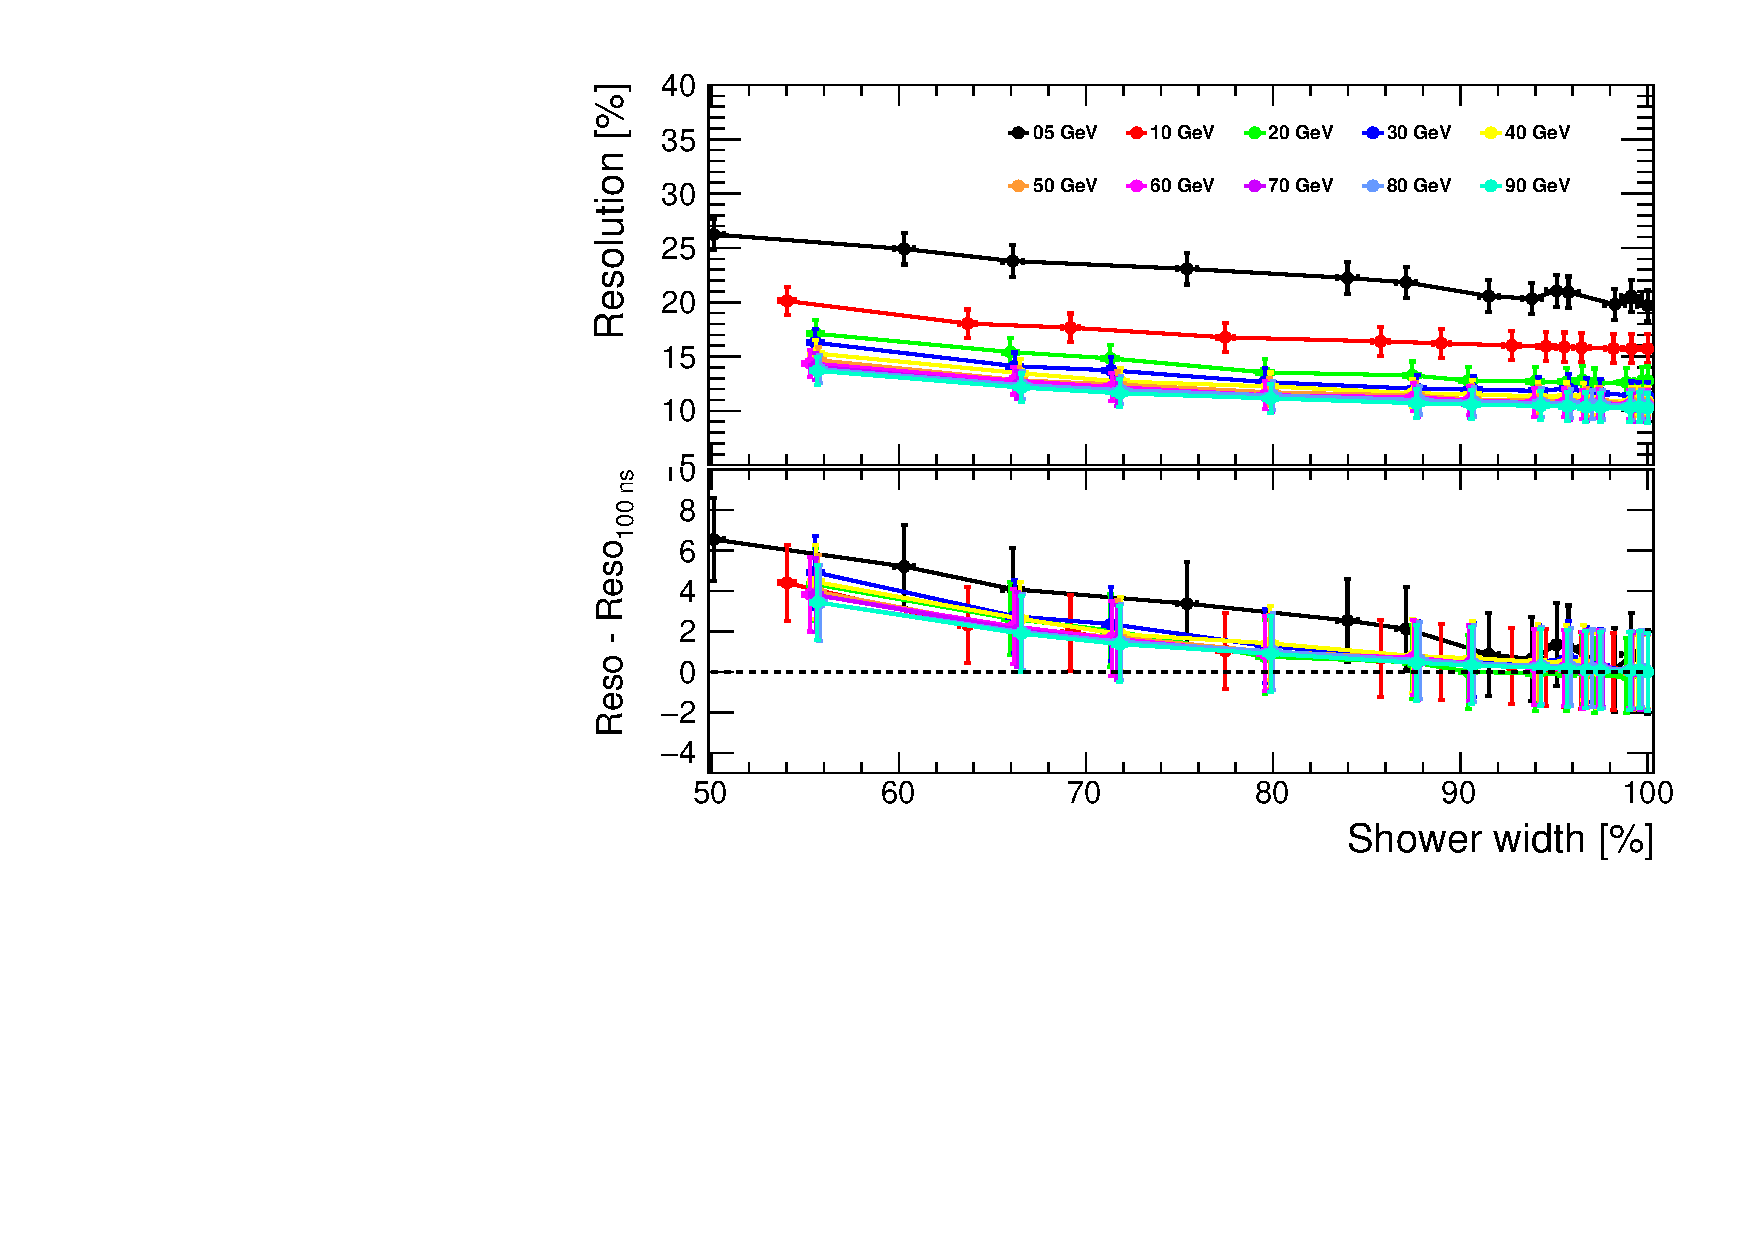
\includegraphics[width=0.7\linewidth]{../Thesis_Plots/ILD/Smearing_0.4ns/Plots/ShowerWidth_Resolution_Smearing1}
  \caption{Energy resolution as function of the shower width for \SI{0.4}{\nano\second} time resolution. The top plot shows the relative energy resolution $\frac{\sigma_{E}}{E}$ for kaons from 5 to 90 \GeV where each point is representing a timing cut as function of the shower width. The bottom plot shows the deviation to the nominal resolution at 100 ns as a function of the shower width.} \label{fig:WidthReso0.4ns}
\end{figure}

\begin{figure}[htbp!]
  \centering
  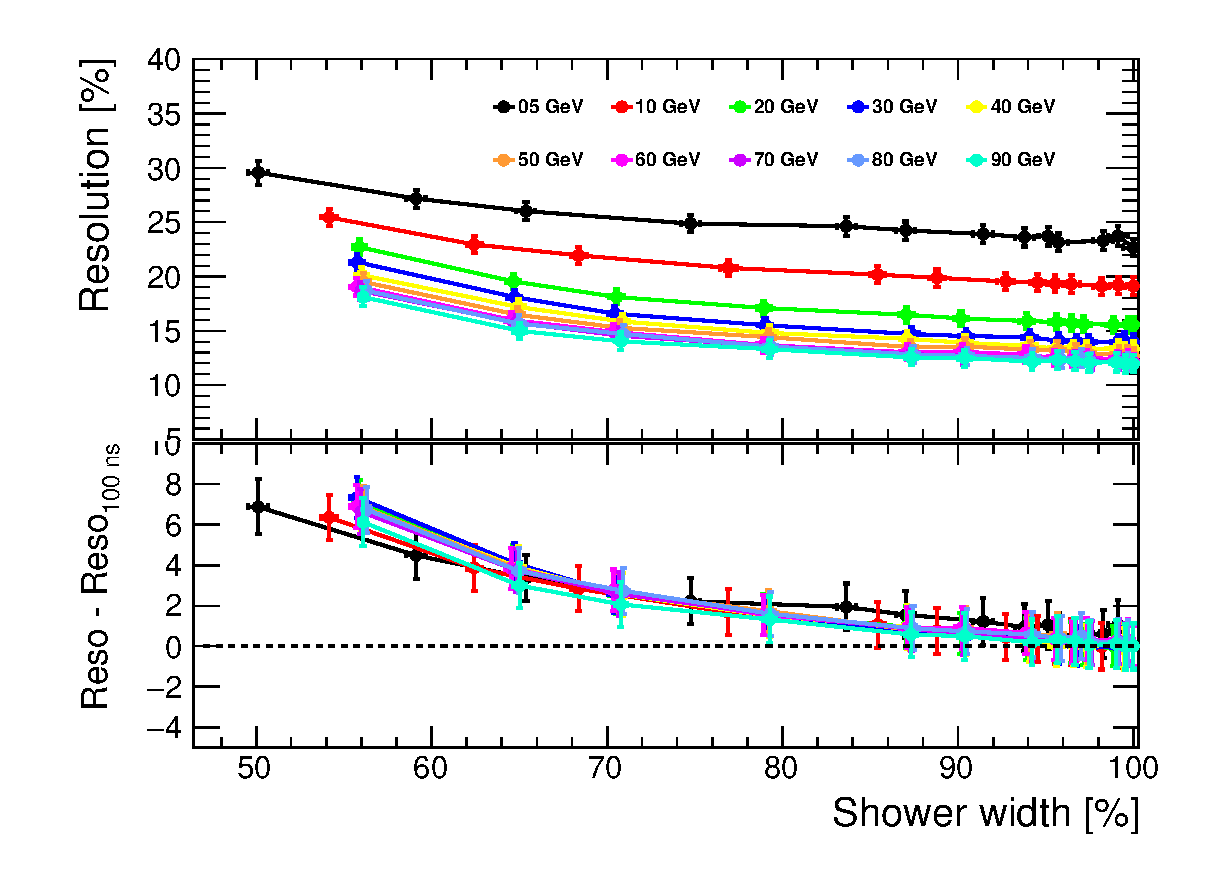
\includegraphics[width=0.7\linewidth]{../Thesis_Plots/ILD/Smearing_1ns/Plots/ShowerWidth_Resolution_Smearing2}
  \caption{Energy resolution as function of the shower width for \SI{1}{\nano\second} time resolution. The top plot shows the relative energy resolution $\frac{\sigma_{E}}{E}$ for kaons from 5 to 90 \GeV where each point is representing a timing cut as function of the shower width. The bottom plot shows the deviation to the nominal resolution at 100 ns as a function of the shower width.} \label{fig:WidthReso1ns}
\end{figure}

\begin{figure}[htbp!]
  \centering
  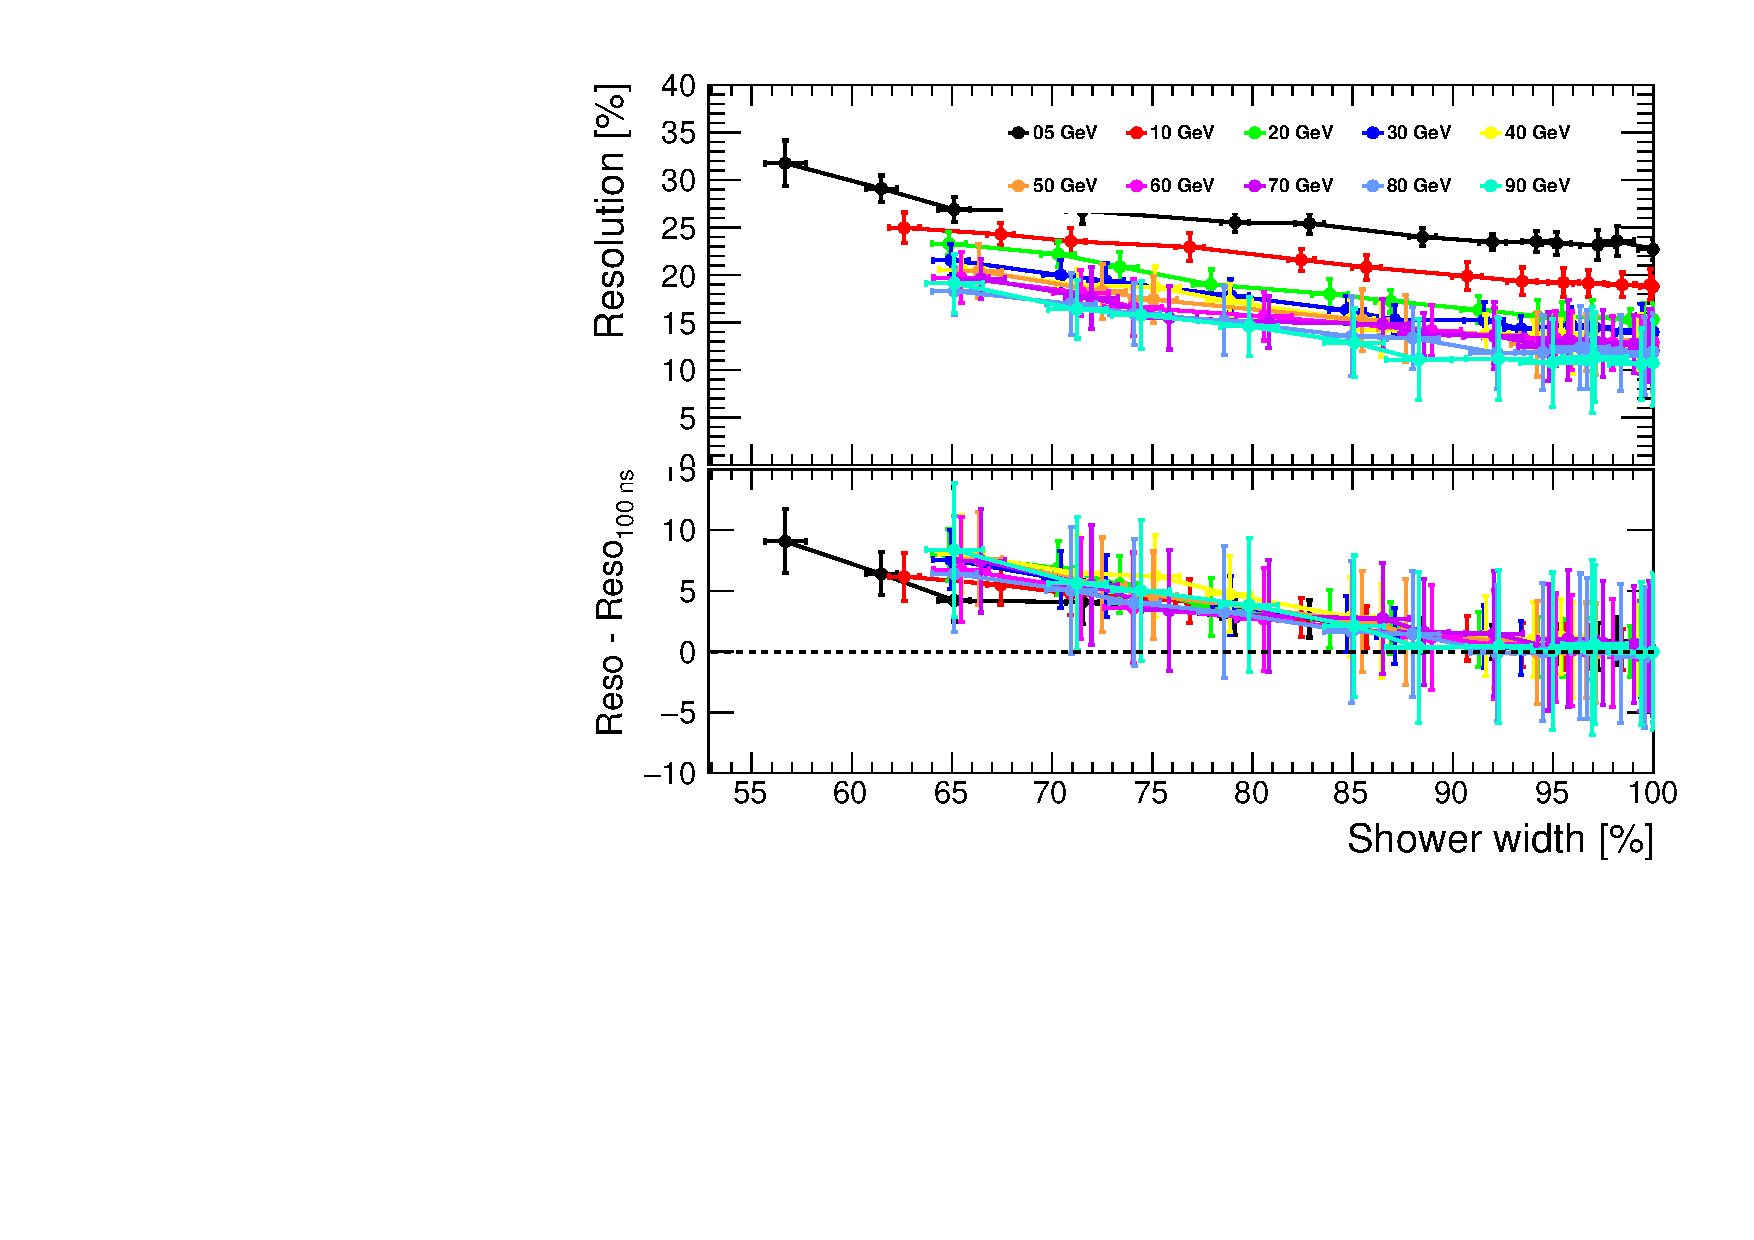
\includegraphics[width=0.7\linewidth]{../Thesis_Plots/ILD/Smearing_8ns/Plots/ShowerWidth_Resolution_Smearing3}
  \caption{Energy resolution as function of the shower width for \SI{8}{\nano\second} time resolution. The top plot shows the relative energy resolution $\frac{\sigma_{E}}{E}$ for kaons from 5 to 90 \GeV where each point is representing a timing cut as function of the shower width. The bottom plot shows the deviation to the nominal resolution at 100 ns as a function of the shower width. The error bars are due to the low amount of statistics available.}  \label{fig:WidthReso8ns}
\end{figure}

\begin{center}
  \rule{0.5\textwidth}{.4pt}
\end{center}

The study presented in this section demonstrates that timing information can be used in hadronic showers in order to improve pattern recognition. This study was performed assuming different time resolutions and shows that in order to benefit from timing information, a time resolution for the electronics in the (sub-)nanosecond scale would be ideal. Assuming a time resolution of 1 ns, a time cut around 1-2 ns would greatly reduce the shower width by about 40\% and would degrade the energy resolution by about 8\% in absolute as well as the linearity by 30\% maximum.

Higher time resolution would certainly help but would impact to a certain level the calorimeter energy resolution. One would need to think how to implement the use of time information in Pandora in order to improve the pattern recognition efficiently.

\section{Understanding the degradation of the energy resolution with timing cuts}
\label{sec:eresdegrad}

To investigate and understand the degradation of the energy resolution with timing cuts, a simple complementary analysis has been done based on the CAN 028 \cite{CaN028}. This CALICE Analysis note presents a software compensation method to improve energy resolution using a correction factor derived from the knowledge of the electromagnetic and hadronic fraction in a shower on an event-by-event basis. It was found that the shape of energy density distributions is correlated with the calorimeter response. The goal of this study is to show that timing cuts favor high electromagnetic fraction events and reduces the correlation.

\subsection{Hit Energy spectra in HCAL}

Due to the high granularity of the HCAL in the ILD detector, a detailed study of hadronic showers is possible at the single cell level (hits). The hadronic calorimeter in ILD is of a non-compensating nature resulting in a higher response for the electromagnetic component of a hadronic shower than for the hadronic component. The $\frac{e}{\pi}$ ratio is around 1.2 \cite{ILC_TDR_Vol4}. Because of this, hadron induced showers with a higher electromagnetic fraction will give a higher response and vice-versa. An example is shown in figure \ref{fig:Response30GeV}. $E_{mean}$ and $\sigma$ correspond to the mean of the distribution and RMS, respectively. The blue subsample contains events reconstructed with $E_{reco} < E_{mean} - \sigma$ and the red one with $E_{reco} > E_{mean} + \sigma$. The corresponding hit energy spectrum is shown in figure \ref{fig:HitSpectra30_100ns}. This shows that the shape of the hit energy spectrum is closely related to the deposited energy. Clusters with a higher reconstructed energy contain hits with larger hit energies which are expected to be mainly caused by the EM component.

\begin{figure}[htbp!]
  \centering
  \begin{subfigure}[t]{0.49\textwidth}
    \centering
    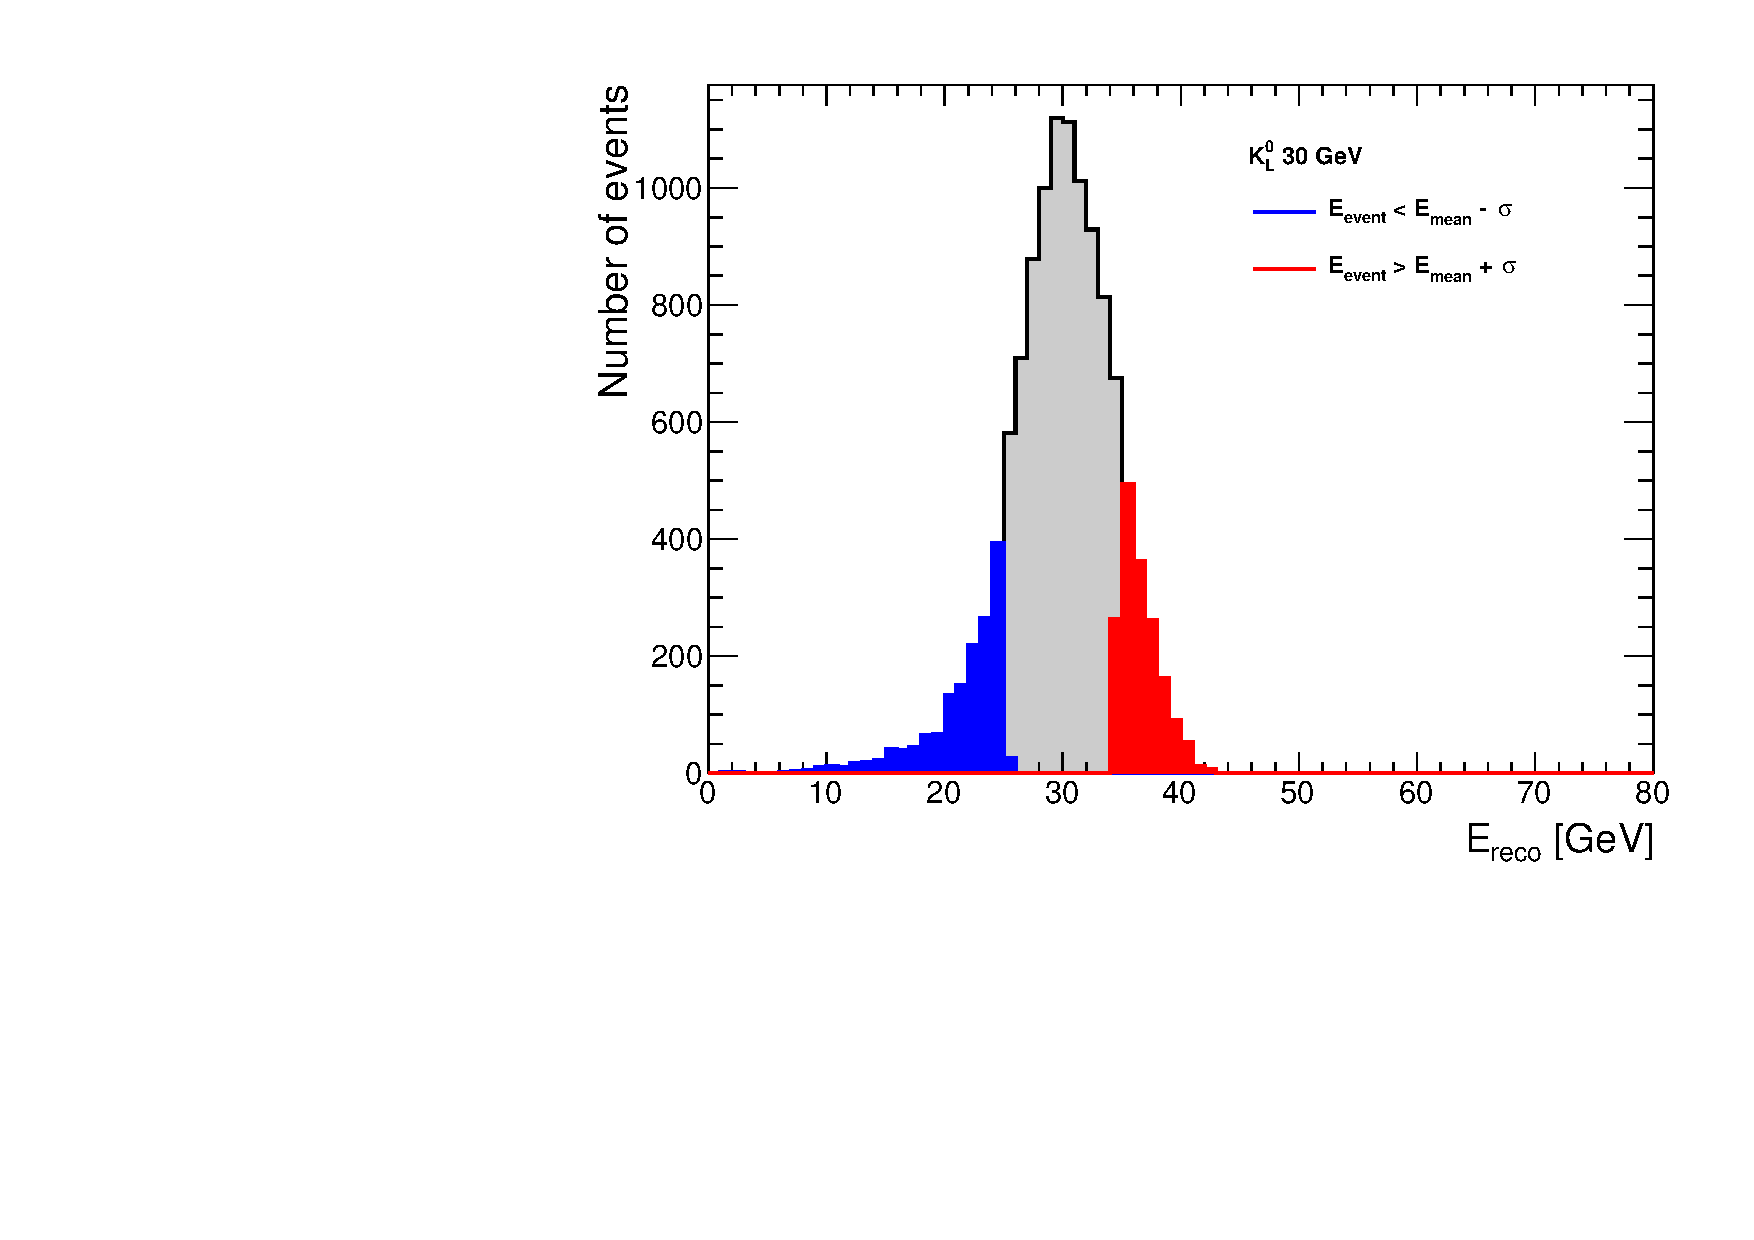
\includegraphics[width=1\linewidth]{../Thesis_Plots/ILD/AdditionalPlots/Plots/EnergySum_100ns_30GeV.pdf}
    \caption{} \label{fig:Esum30_100ns}
  \end{subfigure}
  \hfill
  \begin{subfigure}[t]{0.49\textwidth}
    \centering
    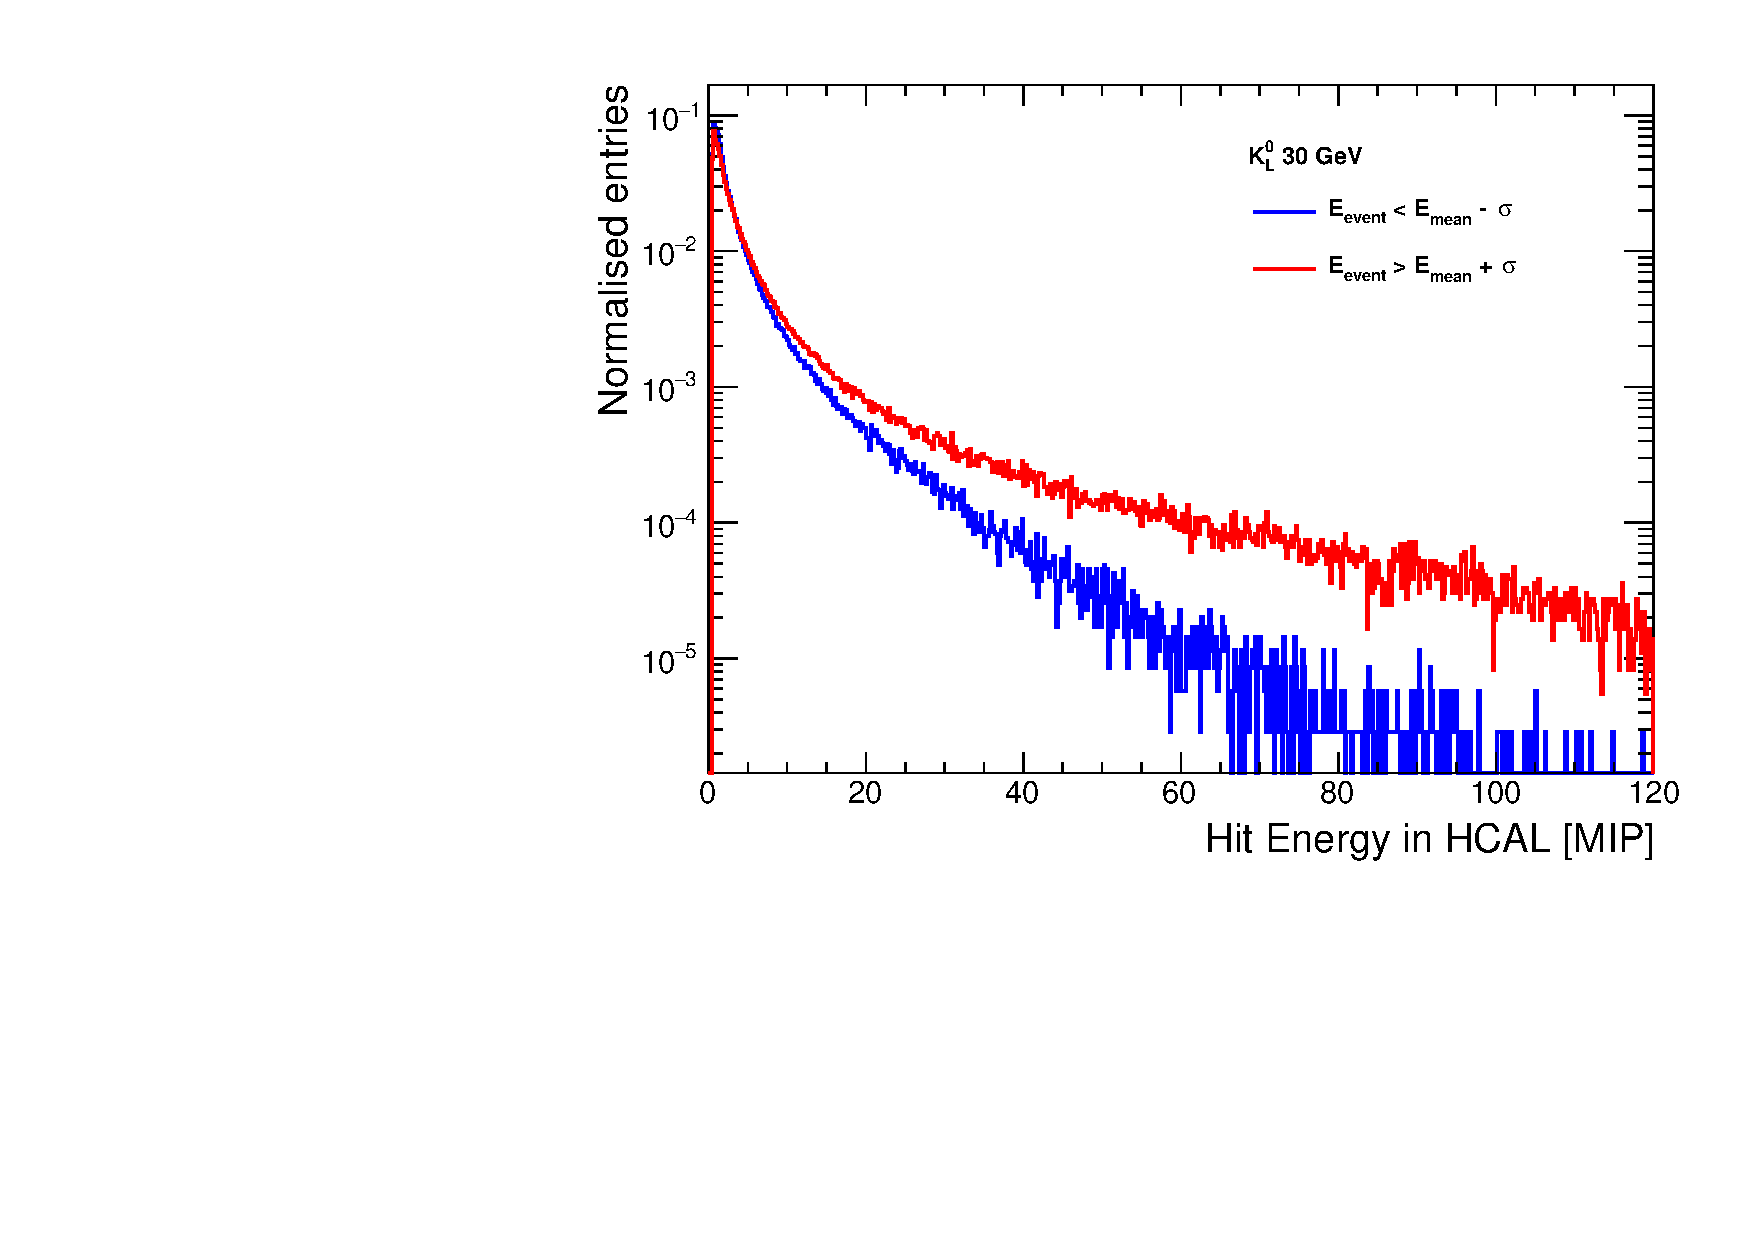
\includegraphics[width=1\linewidth]{../Thesis_Plots/ILD/AdditionalPlots/Plots/HitEnergySpectra_100ns_30GeV.pdf}
    \caption{} \label{fig:HitSpectra30_100ns}
  \end{subfigure}
  \caption{\subref{fig:Esum30_100ns}) Reconstructed energy distribution for 30 GeV kaons. \subref{fig:HitSpectra30_100ns}) Associated hit energy spectrum in the HCAL corresponding to subsamples with low (in blue) and high (in red) energy depositions.} \label{fig:Response30GeV}
\end{figure}

Following the CAN 028, a quantitative probability $C_{i}^{lim}$ of the i-th event was obtained as follows:
\begin{equation}
  C_{i}^{lim} = \frac{N_{i}(e \leq e^{lim})}{N_{i}^{HCAL}}
\end{equation}

where $N_{i}(e \leq e^{lim})$ is the number of hits with energy $e \leq e^{lim}$ and $N_{i}^{HCAL}$ the number of hits in the HCAL. The value of $e^{lim}$ is in an interval of 3 to 5 MIPs and was observed for the intersection of hit energy spectra for kaons between 10 and 80 GeV. A zoom between 0 and 14 MIP for 30 GeV is shown in figure \ref{fig:HitSpectra30_Zoom_100ns}.

\begin{figure}[htbp!]
  \centering
  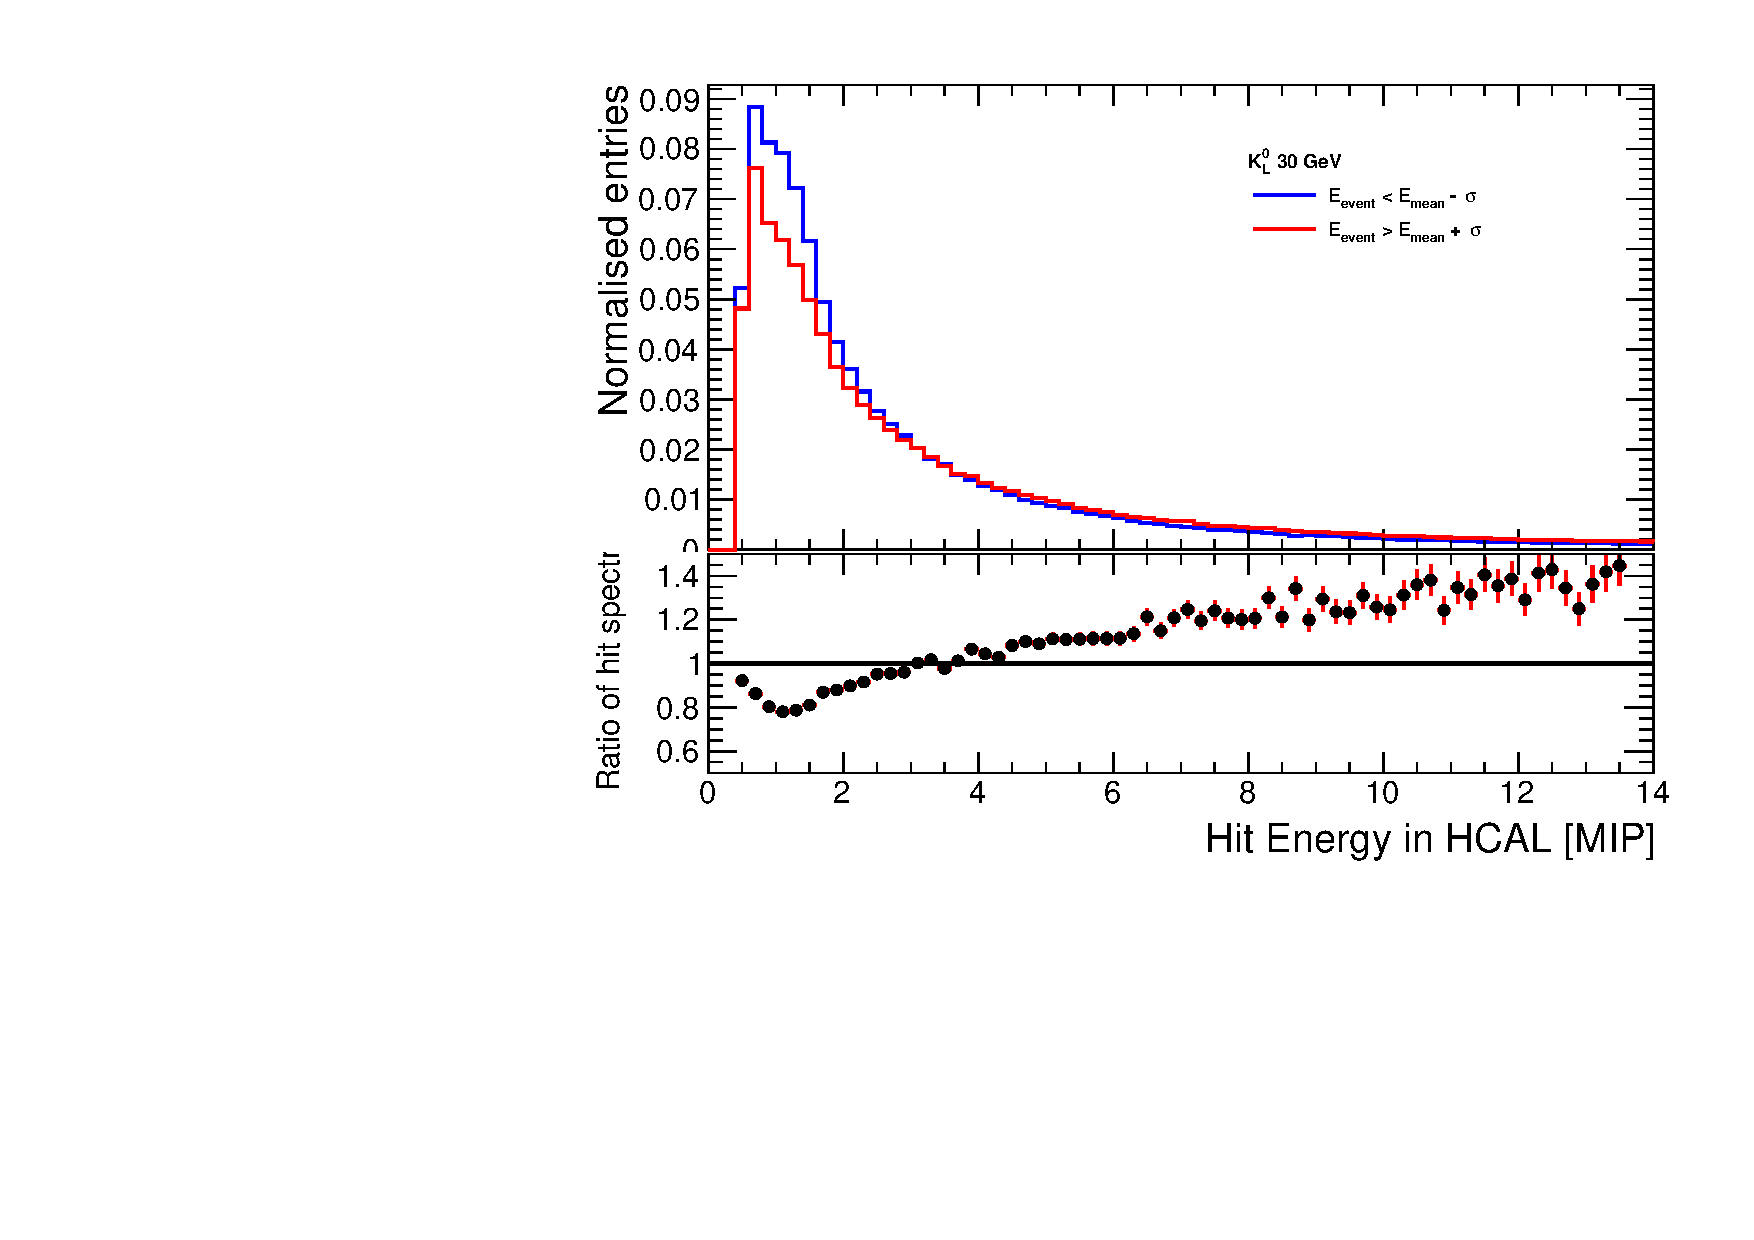
\includegraphics[width=0.7\linewidth]{../Thesis_Plots/ILD/AdditionalPlots/Plots/HitEnergySpectra_Zoom_100ns_30GeV.pdf}
  \caption{The top plot shows the hit energy spectrum in the HCAL for 30 GeV kaons for the subsample low (blue) and high (red) of energy depositions. The bottom plot shows the ratio of the red to the blue spectrum.} \label{fig:HitSpectra30_Zoom_100ns}
\end{figure}

The distribution of $C^{lim}$ for different values of $e^{lim}$ are shown in figure \ref{fig:CLim30_100ns} for 30 GeV kaons. One can see that the distributions get narrower with increasing $e^{lim}$. By choosing the right value of $e^{lim}$, it may be possible to distinguish between the red and blue subsamples by their $C^{lim}$ distributions. For this analysis, a value of 3.5 MIP was chosen for $e^{lim}$. One can observe that for events where the reconstructed energy is below $E_{mean} - \sigma$ correspond to a higher value of $C^{lim}$ and vice-versa. The blue distribution has a mean of 0.71 and the red distribution has a mean of 0.61, this corresponds to a separation of 14.1\%.

\begin{figure}[htbp!]
  \centering
  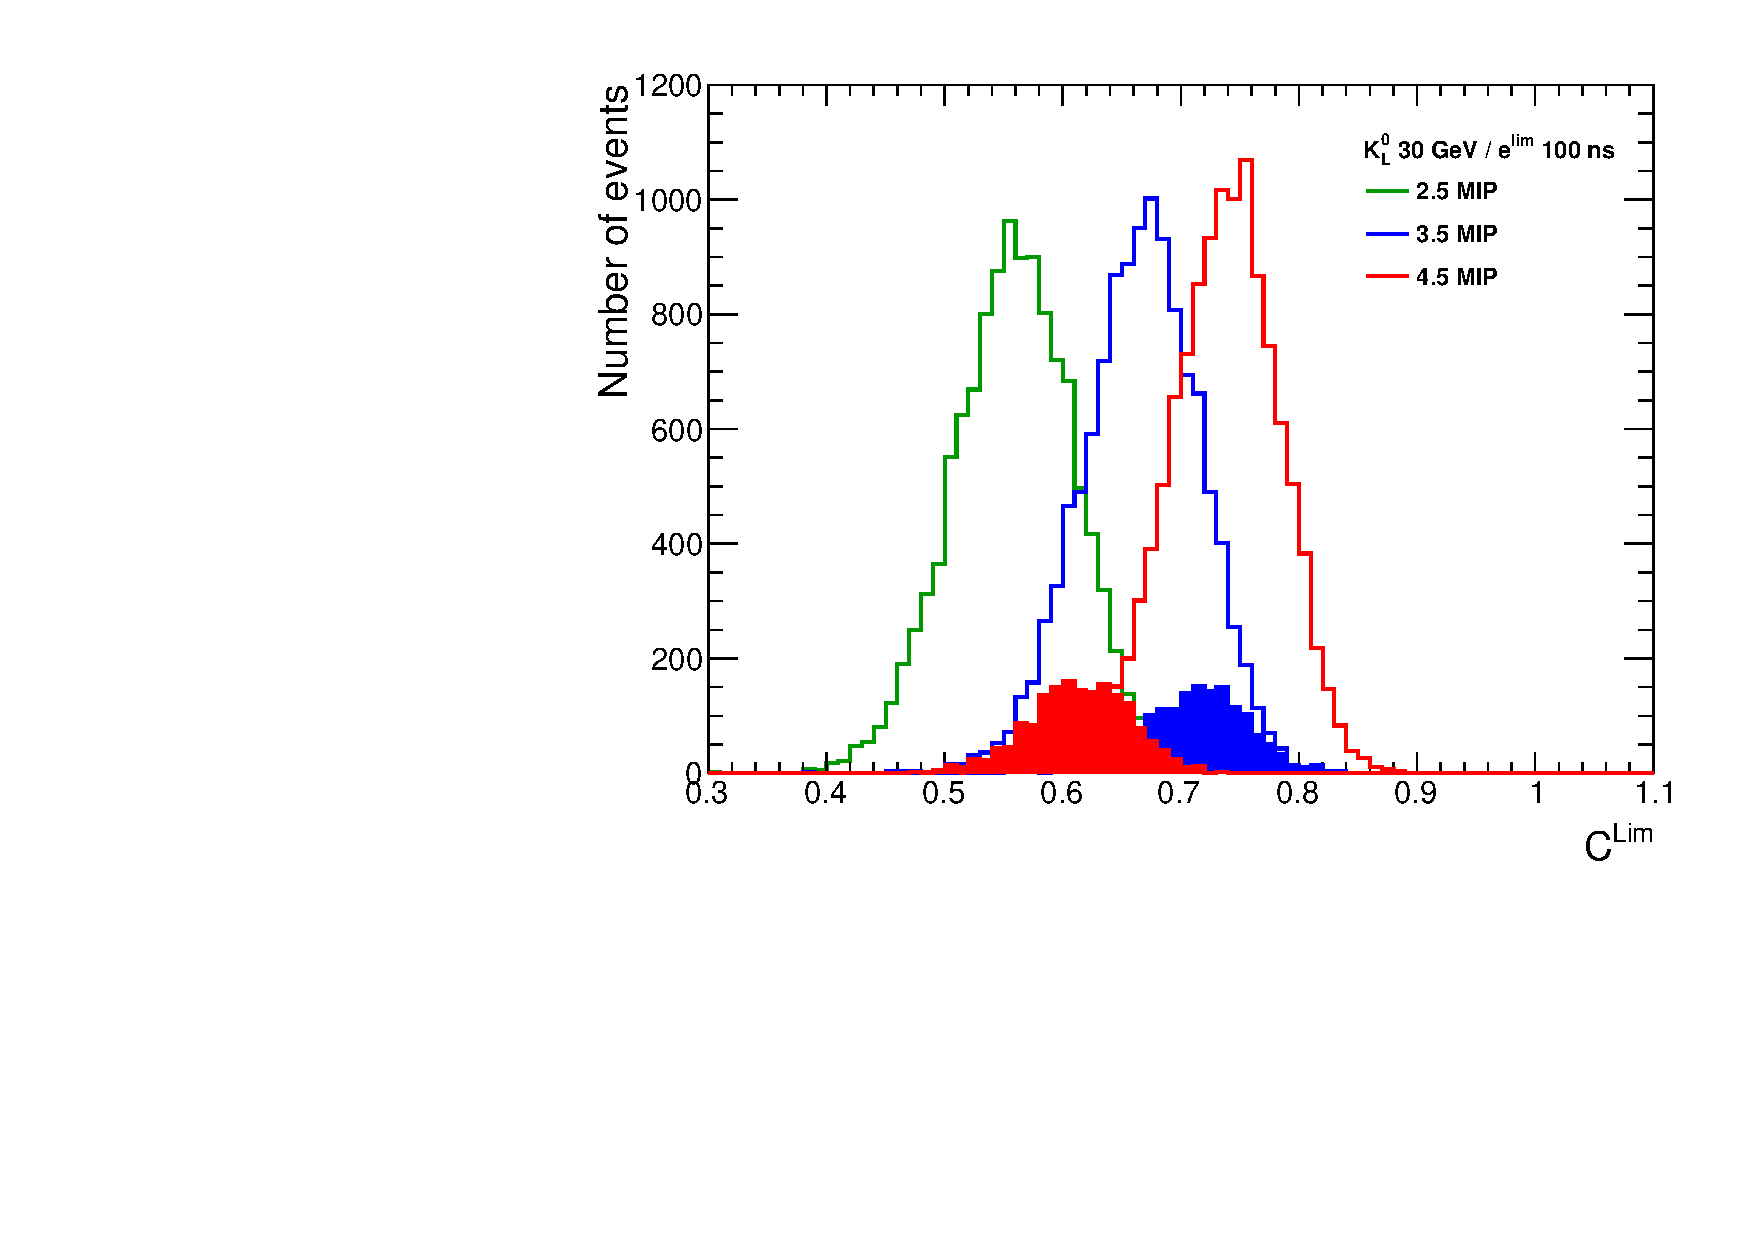
\includegraphics[width=0.7\linewidth]{../Thesis_Plots/ILD/AdditionalPlots/Plots/CLim_100ns_30GeV.pdf}
  \caption{Distributions of $C^{lim}$ for different values of $e^{lim}$ for 30 GeV kaons. The red and blue filled histograms corresponds to events that are in the region $E_{mean} \pm \sigma$ respectively.} \label{fig:CLim30_100ns}
\end{figure}

An inverse correlation is found between the total energy in the HCAL and $C^{lim}$ as shown in figure \ref{fig:EhcalCLim30_100ns}. The inverse correlation is much stronger for higher kaon energies and becomes weaker with lower energies.

\begin{figure}[htbp!]
  \centering
  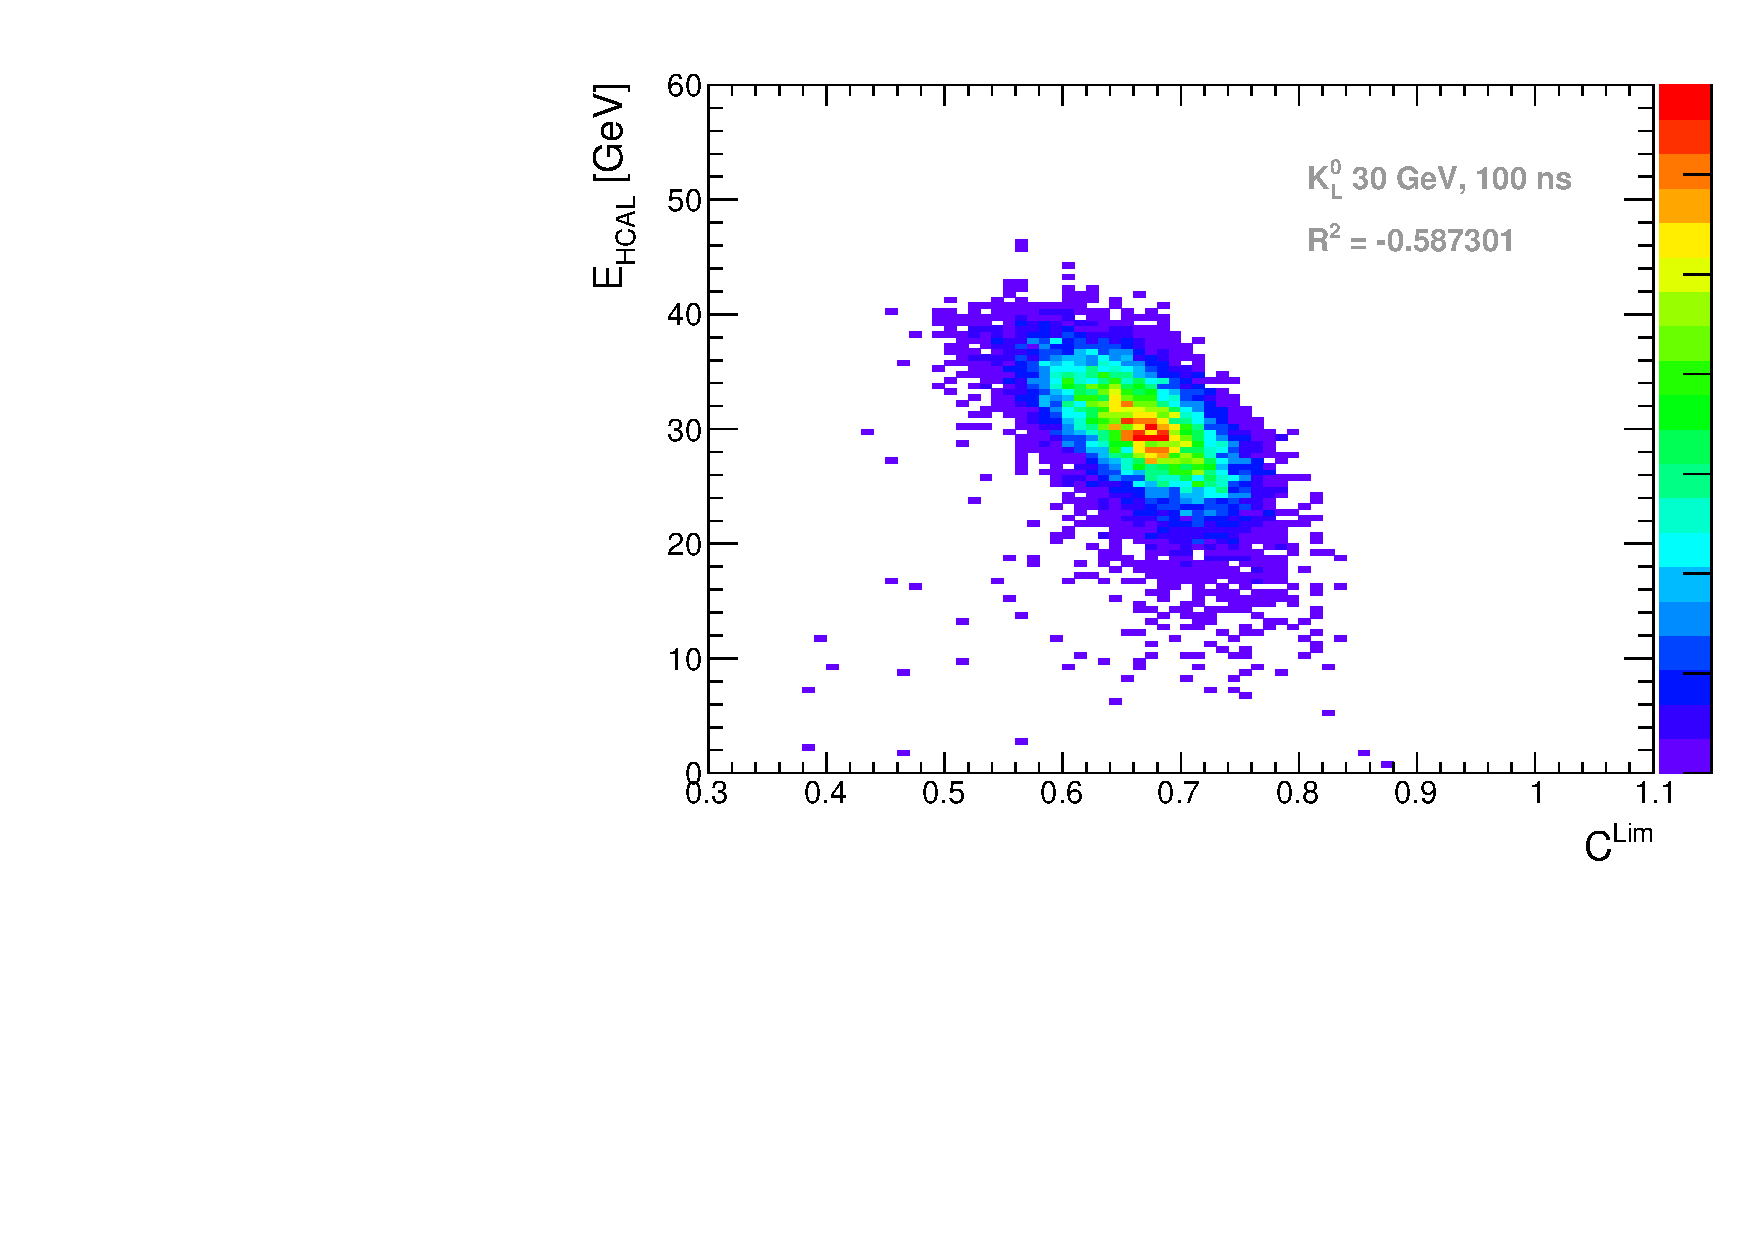
\includegraphics[width=0.7\linewidth]{../Thesis_Plots/ILD/AdditionalPlots/Plots/EhcalCLim_100ns_30GeV.pdf}
  \caption{Correlation between the energy deposited in the HCAL for 30 GeV kaons and $C^{lim}$ for $e^{lim}$ = 3.5 MIPs.} \label{fig:EhcalCLim30_100ns}
\end{figure}

% \begin{figure}[htbp!]
%   \centering
%   \begin{subfigure}[t]{0.49\textwidth}
%     \centering
%     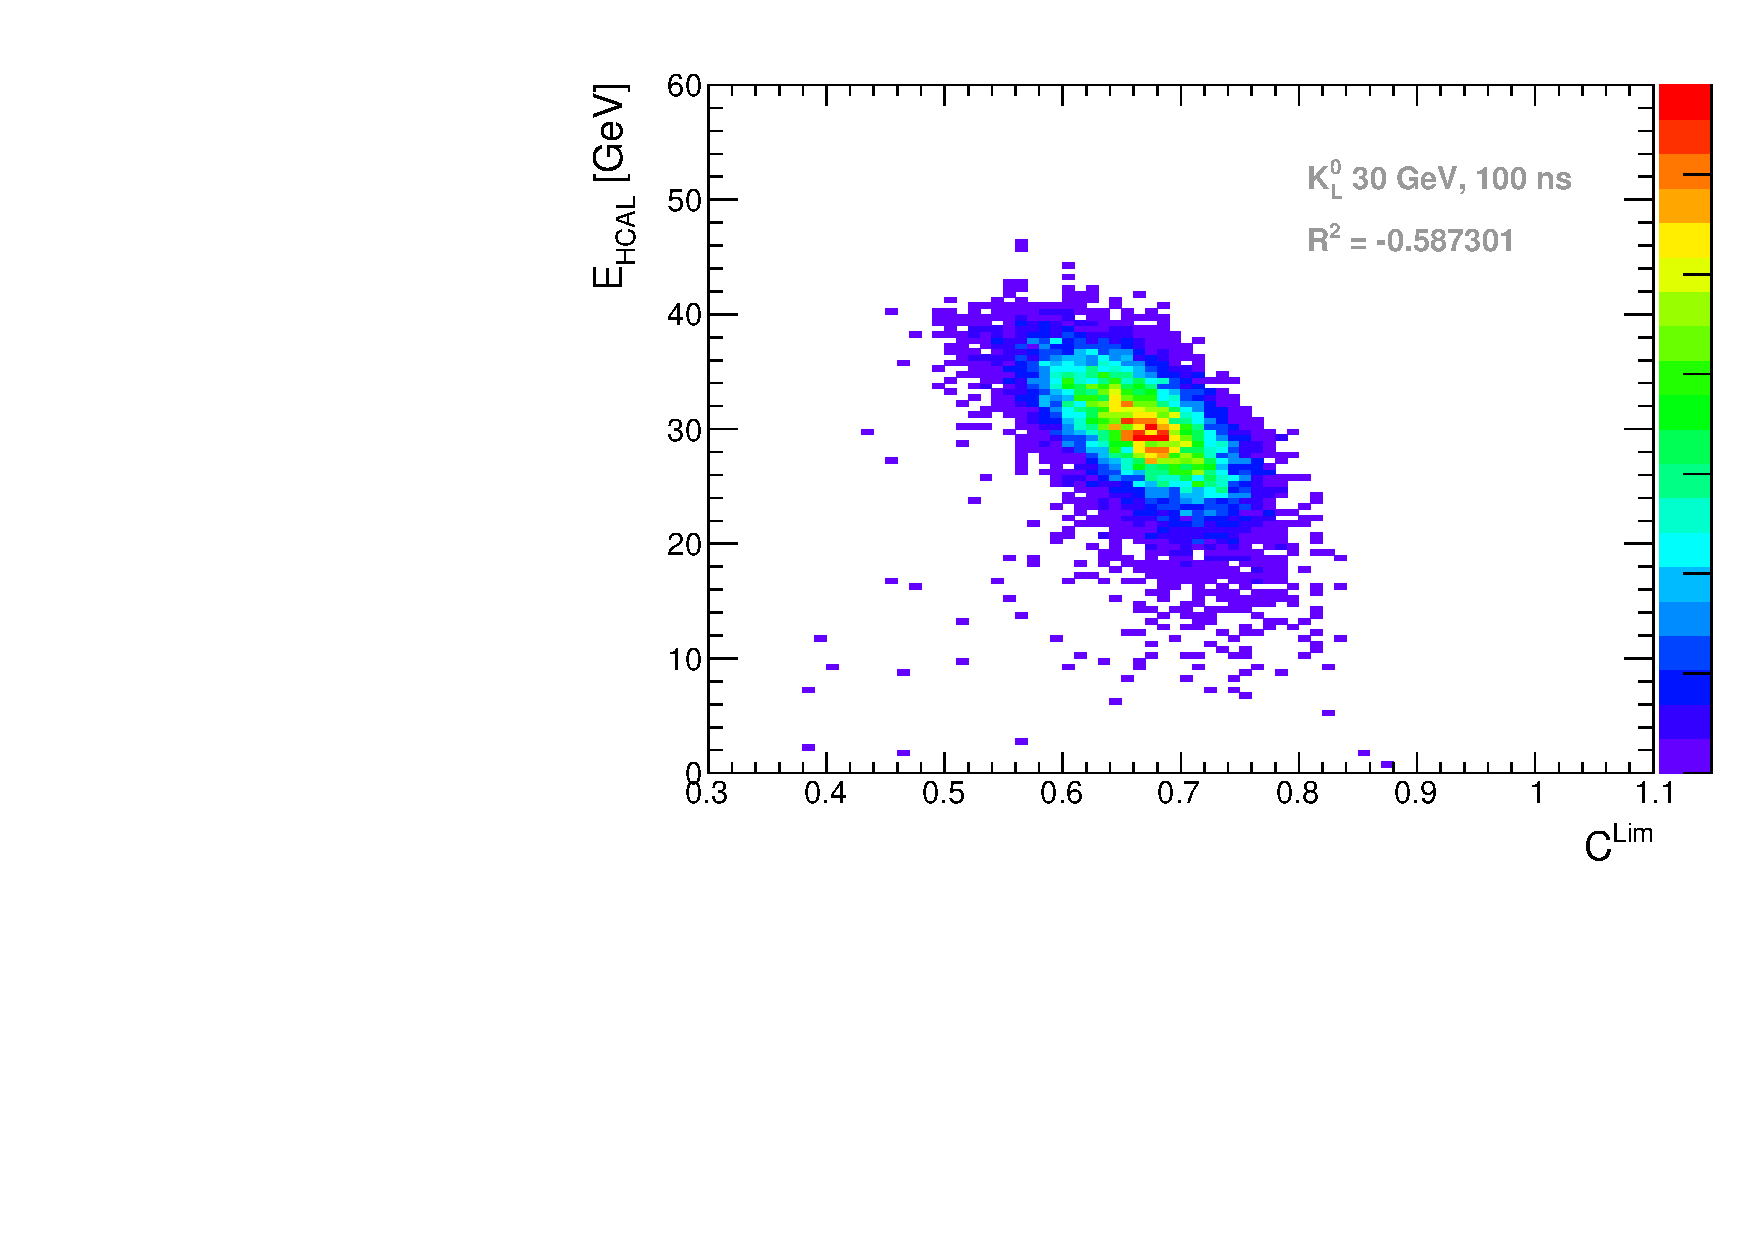
\includegraphics[width=1\linewidth]{../Thesis_Plots/ILD/AdditionalPlots/Plots/EhcalCLim_100ns_30GeV.pdf}
%     \caption{30 GeV.} \label{fig:EhcalCLim30_100ns}
%   \end{subfigure}
%   \hfill
%   \begin{subfigure}[t]{0.49\textwidth}
%     \centering
%     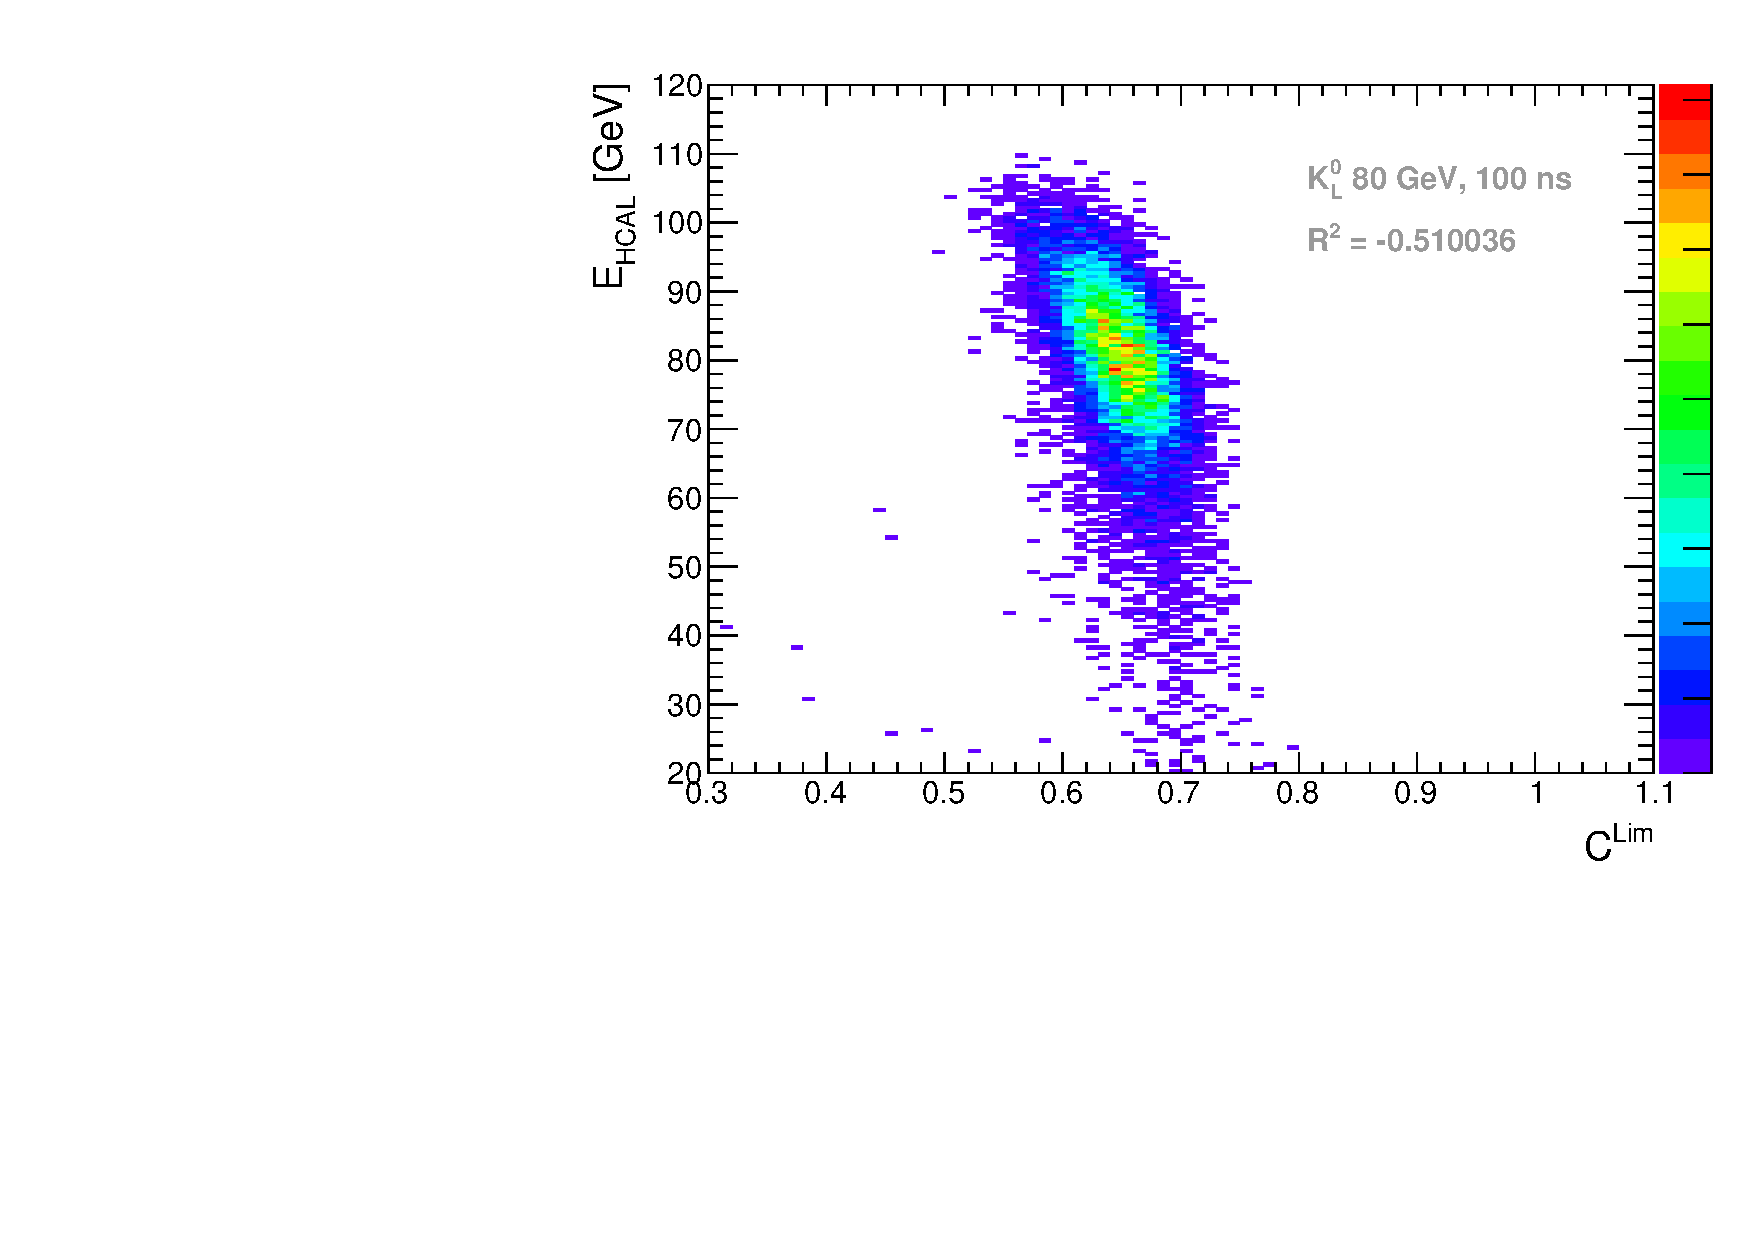
\includegraphics[width=1\linewidth]{../Thesis_Plots/ILD/AdditionalPlots/Plots/EhcalCLim_100ns_80GeV.pdf}
%     \caption{80 GeV.} \label{fig:EhcalCLim80_100ns}
%   \end{subfigure}
%   \caption{\subref{fig:EhcalCLim30_100ns}) Correlation between the energy deposited in the HCAL for 30 GeV kaons and $C^{lim}$ for $e^{lim}$ = 3.5 MIPs. \subref{fig:EhcalCLim80_100ns}) Correlation between the energy deposited in the HCAL for 80 GeV kaons and $C^{lim}$ for $e^{lim}$ = 3.5 MIPs.}
% \end{figure}

In a next step, timing cut will be applied and a comparison with these results will be done. It is believed that timing cuts will have an effect of narrowing the $C^{lim}$ distributions, thus bringing the blue $C^{lim}$ distribution (hadronic component) closer to the red $C^{lim}$ distribution (EM component). Therefore reducing the inverse correlation of $C^{lim}$ with the energy deposited as fluctuation are cut down by timing cuts thus would favor higher electromagnetic fraction hadronic showers.

\subsection{Influence of timing cuts on hit energy spectra in HCAL}

A check was performed on the shape of the hit spectra in the HCAL with different timing cuts. The figure \ref{fig:HitSpectra30_timingcuts} shows the hit spectra for 30 GeV kaons with a timing cut of 100 and 1 ns. The green line in the bottom plot represents the value of $e^{lim}$ = 3.5 MIPs.

% \begin{figure}[htbp!]
%   \centering
%   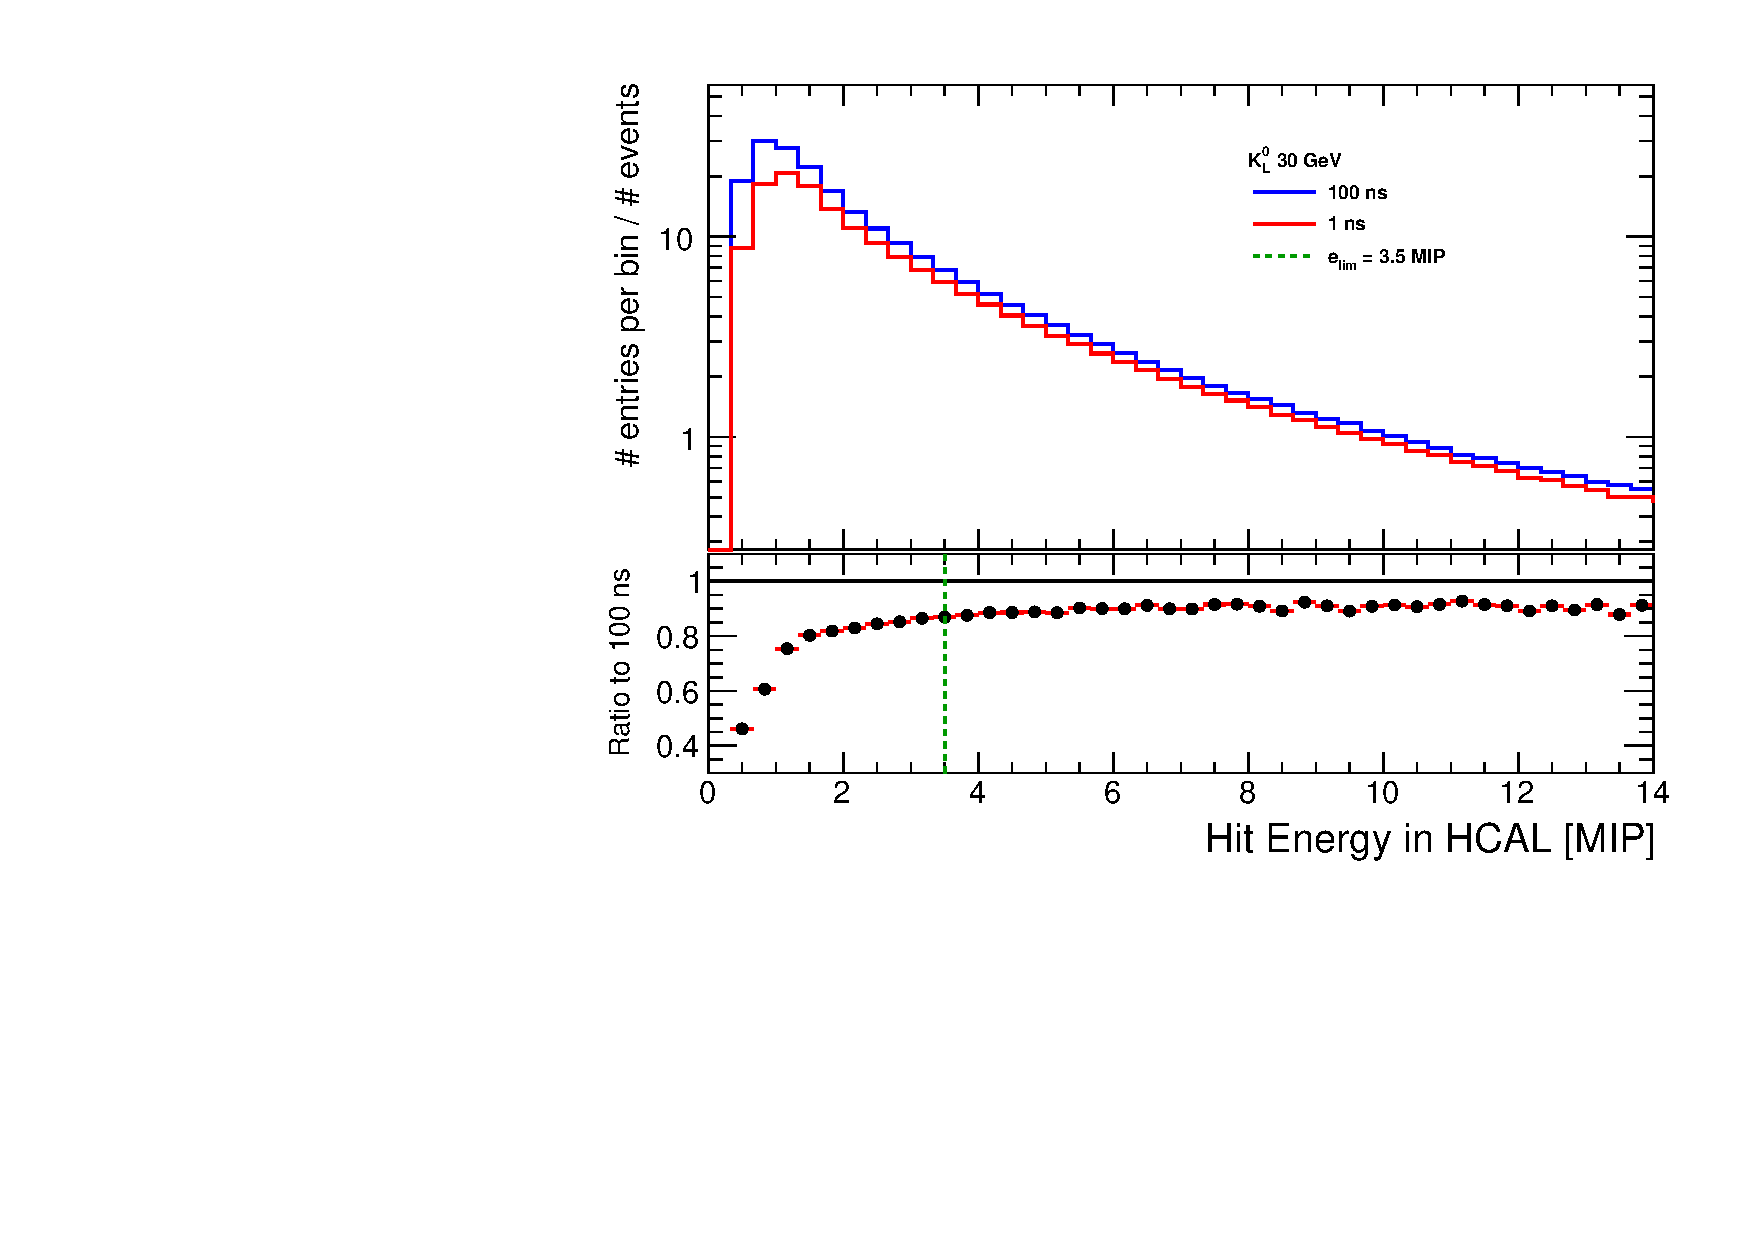
\includegraphics[width=0.7\linewidth]{../Thesis_Plots/ILD/AdditionalPlots/Plots/HitEnergySpectra_Comparison_30GeV.pdf}
%   \caption{The upper plot shows the hit energy spectra in the HCAL for 30 GeV kaons with different timing cuts applied. The bottom plot shows the ratio of the spectra compared to 100 ns.} \label{fig:HitSpectra30_timingcuts}
% \end{figure}

\begin{figure}[htbp!]
  \centering
  \begin{subfigure}[t]{0.49\textwidth}
    \centering
    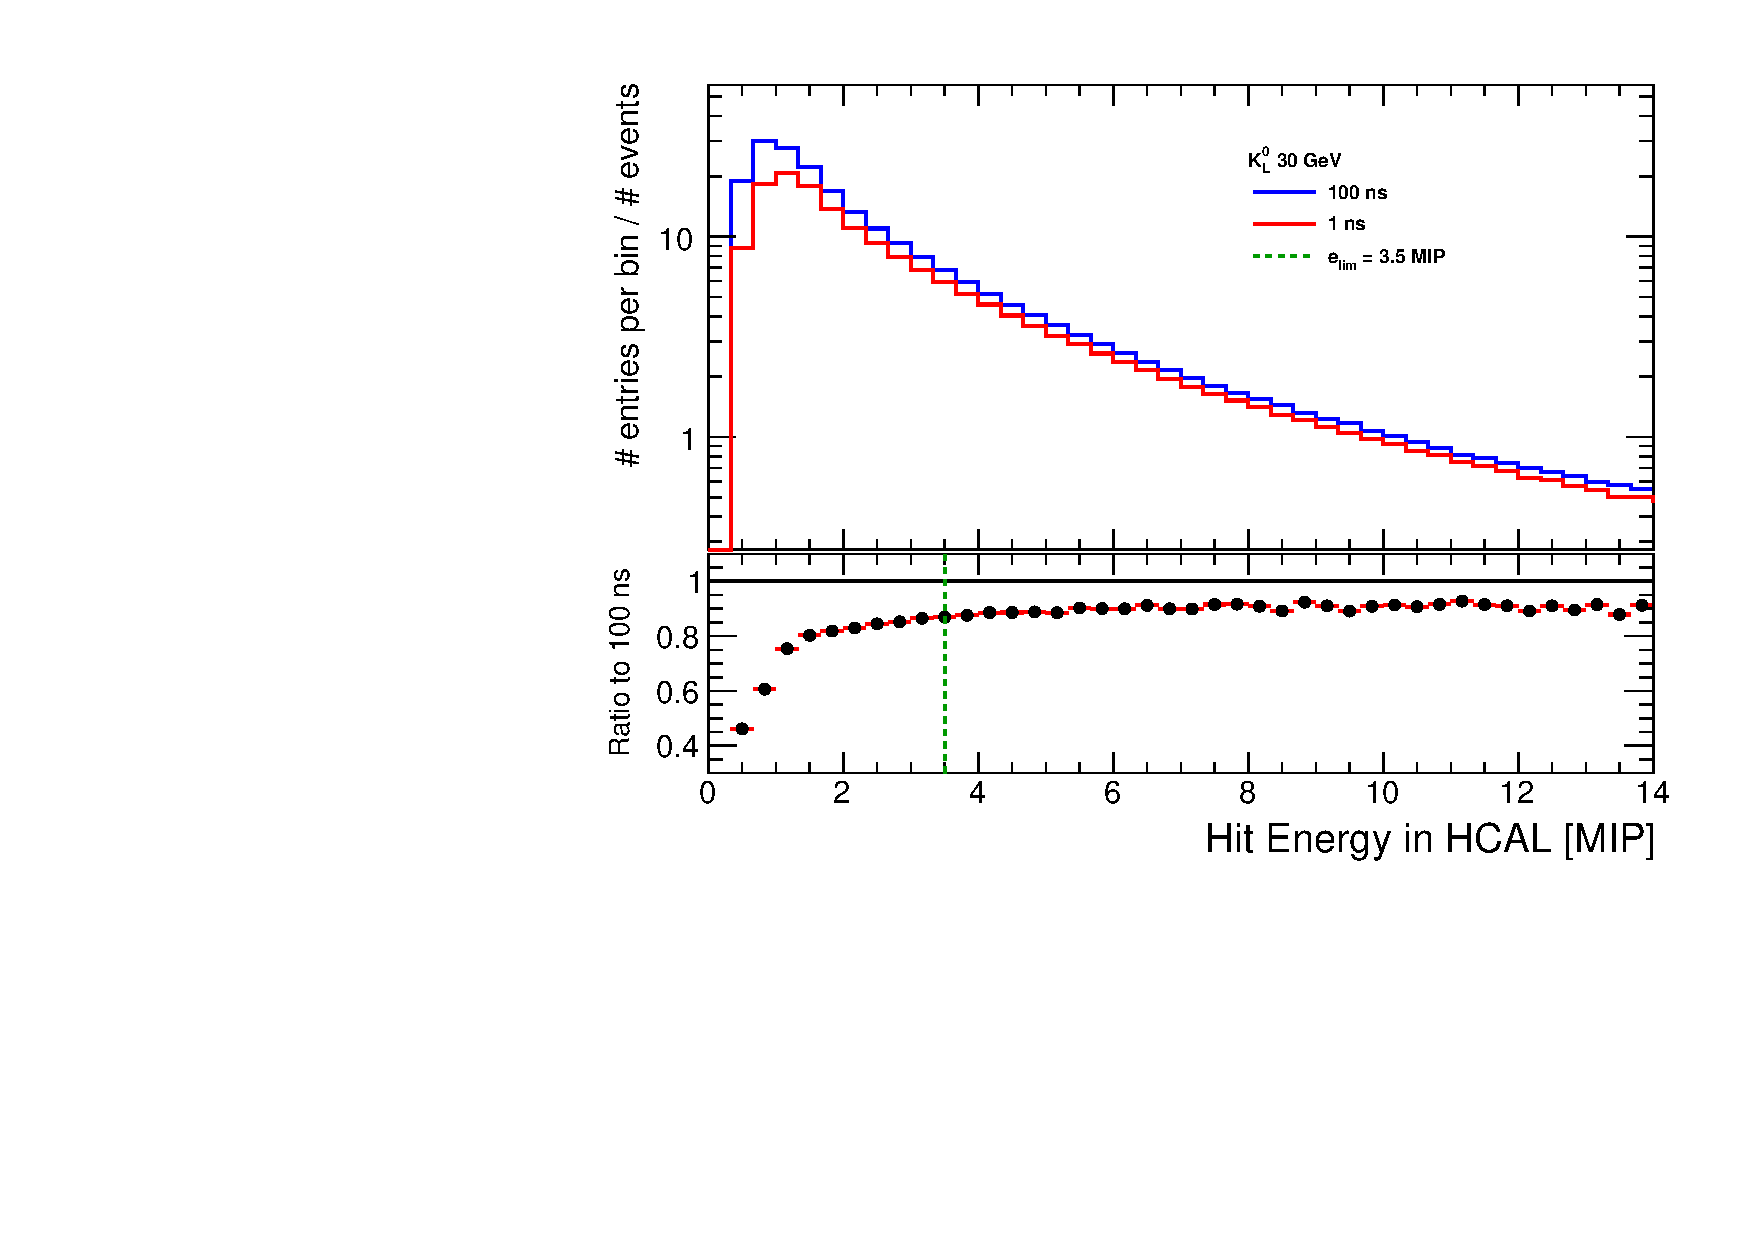
\includegraphics[width=1\linewidth]{../Thesis_Plots/ILD/AdditionalPlots/Plots/HitEnergySpectra_Comparison_30GeV.pdf}
    \caption{30 GeV.} \label{fig:HitSpectra30_timingcuts}
  \end{subfigure}
  \hfill
  \begin{subfigure}[t]{0.49\textwidth}
    \centering
    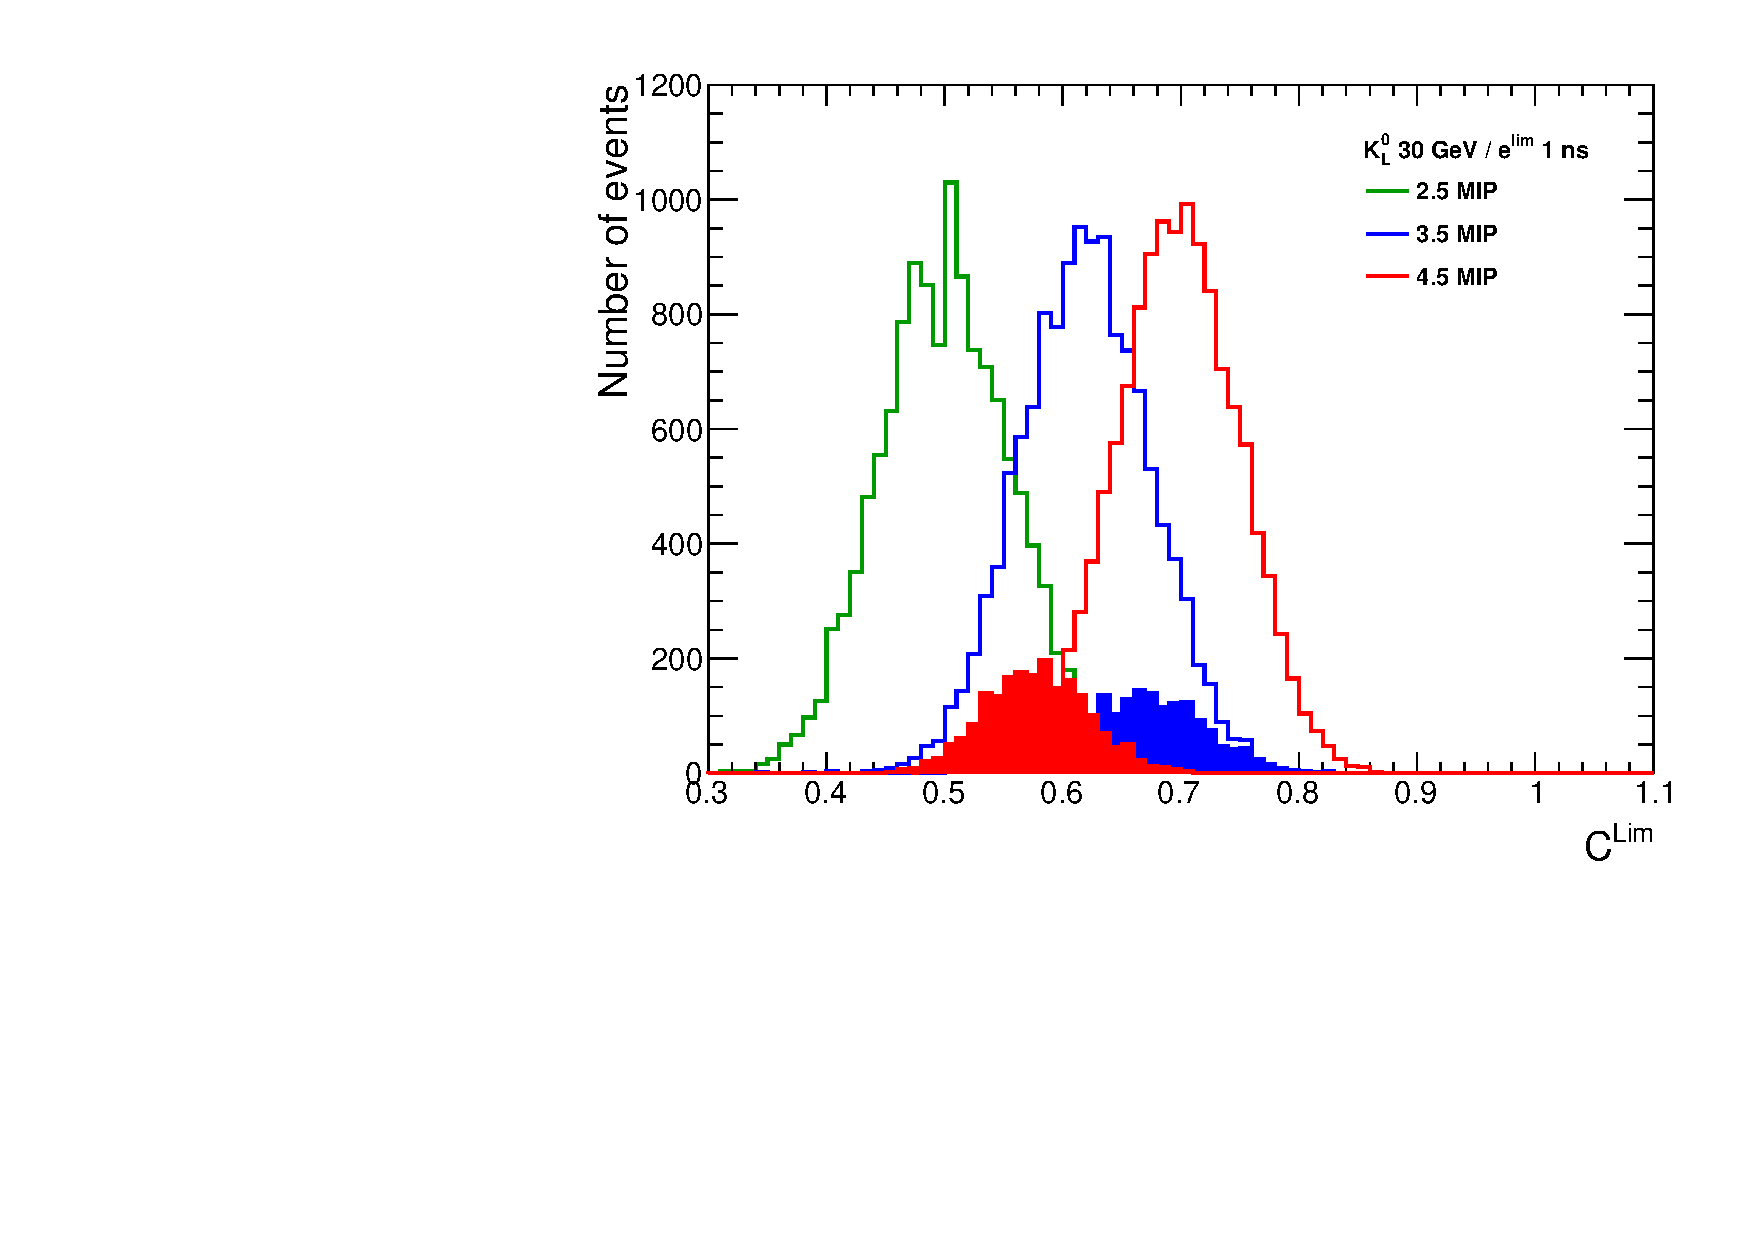
\includegraphics[width=1\linewidth]{../Thesis_Plots/ILD/AdditionalPlots/Plots/CLim_1ns_30GeV.pdf}
    \caption{80 GeV.} \label{fig:CLim30_1ns}
  \end{subfigure}
  \caption{\subref{fig:HitSpectra30_timingcuts}) The upper plot shows the hit energy spectra in the HCAL for 30 GeV kaons with different timing cuts applied. The bottom plot shows the ratio of the spectra compared to 100 ns. \subref{fig:CLim30_1ns}) Distributions of $C^{lim}$ for different values of $e^{lim}$ for 30 GeV kaons for 1 ns timing cut. The red and blue filled histograms corresponds to events that are in the region $E_{mean} \pm \sigma$ respectively.}
\end{figure}

One can notice that the shape of the spectra differs slightly with timing cuts. A large reduction of low energy hits ($\sim$1 MIP) is visible. With a cut of 1 ns, there are around 10\% less hits over 4 MIPs but up to 60\% less hits below 1 MIP. With a value of 3.5 MIP for $e^{lim}$, it seems that there are globally fewer hits below, thus reducing the value of $C^{lim}$. A lower value of $C^{lim}$ would correspond to a higher energy deposited thus giving a hint that timing cuts enhance the electromagnetic response of the calorimeter making even more non-compensating. This is shown in figure \ref{fig:CLim30_1ns}.

% \begin{figure}[htbp!]
%   \centering
%   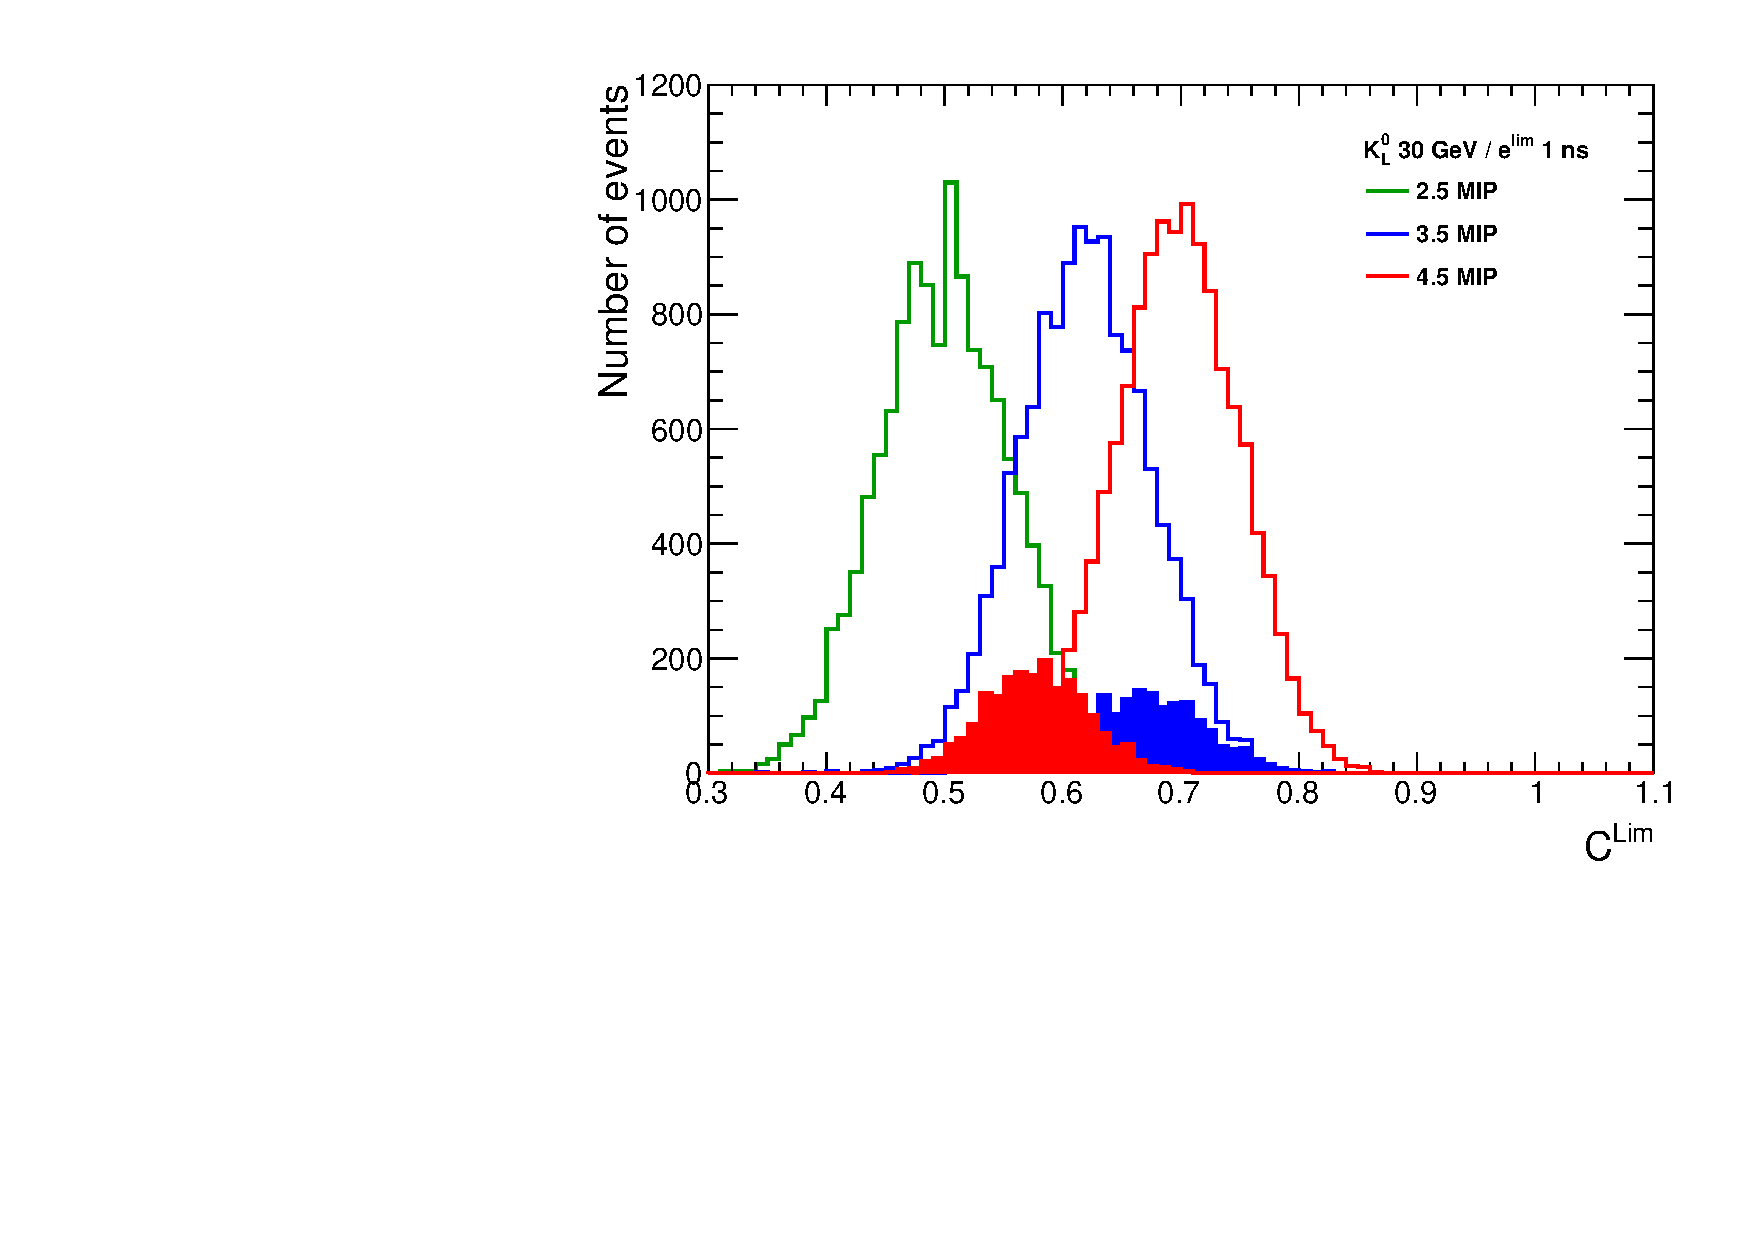
\includegraphics[width=0.7\linewidth]{../Thesis_Plots/ILD/AdditionalPlots/Plots/CLim_1ns_30GeV.pdf}
%   \caption{Distributions of $C^{lim}$ for different values of $e^{lim}$ for 30 GeV kaons for 1 ns timing cut. The blue and red filled histograms corresponds to events that are in the region $E_{mean} \pm \sigma$ respectively.} \label{fig:CLim30_1ns}
% \end{figure}

The blue $C^{lim}$ distribution has a mean of 0.66 and the red $C^{lim}$ distribution has a mean of 0.58. This corresponds to a separation of 12.1\%. The timing cut of 1 ns has the effect of reducing the distance between both distributions by around 2\%. To further confirm this observation, the same correlation plots between the energy deposited in the HCAL and $C^{lim}$ is shown in figure \ref{fig:EhcalCLim30_1ns} for 1 ns timing cut. The anti-correlation is reduced slightly with the correlation coefficient going from -0.58 to -0.48 and the distribution looks more circular. This further confirms that the timing cuts reduce the fluctuations between the electromagnetic and hadronic fractions in hadronic showers by cutting the hadronic response and enhancing the electromagnetic one. This has an effect of non-compensation in the response to hadronic showers thus degrading the energy resolution furthermore.

\begin{figure}[htbp!]
  \centering
  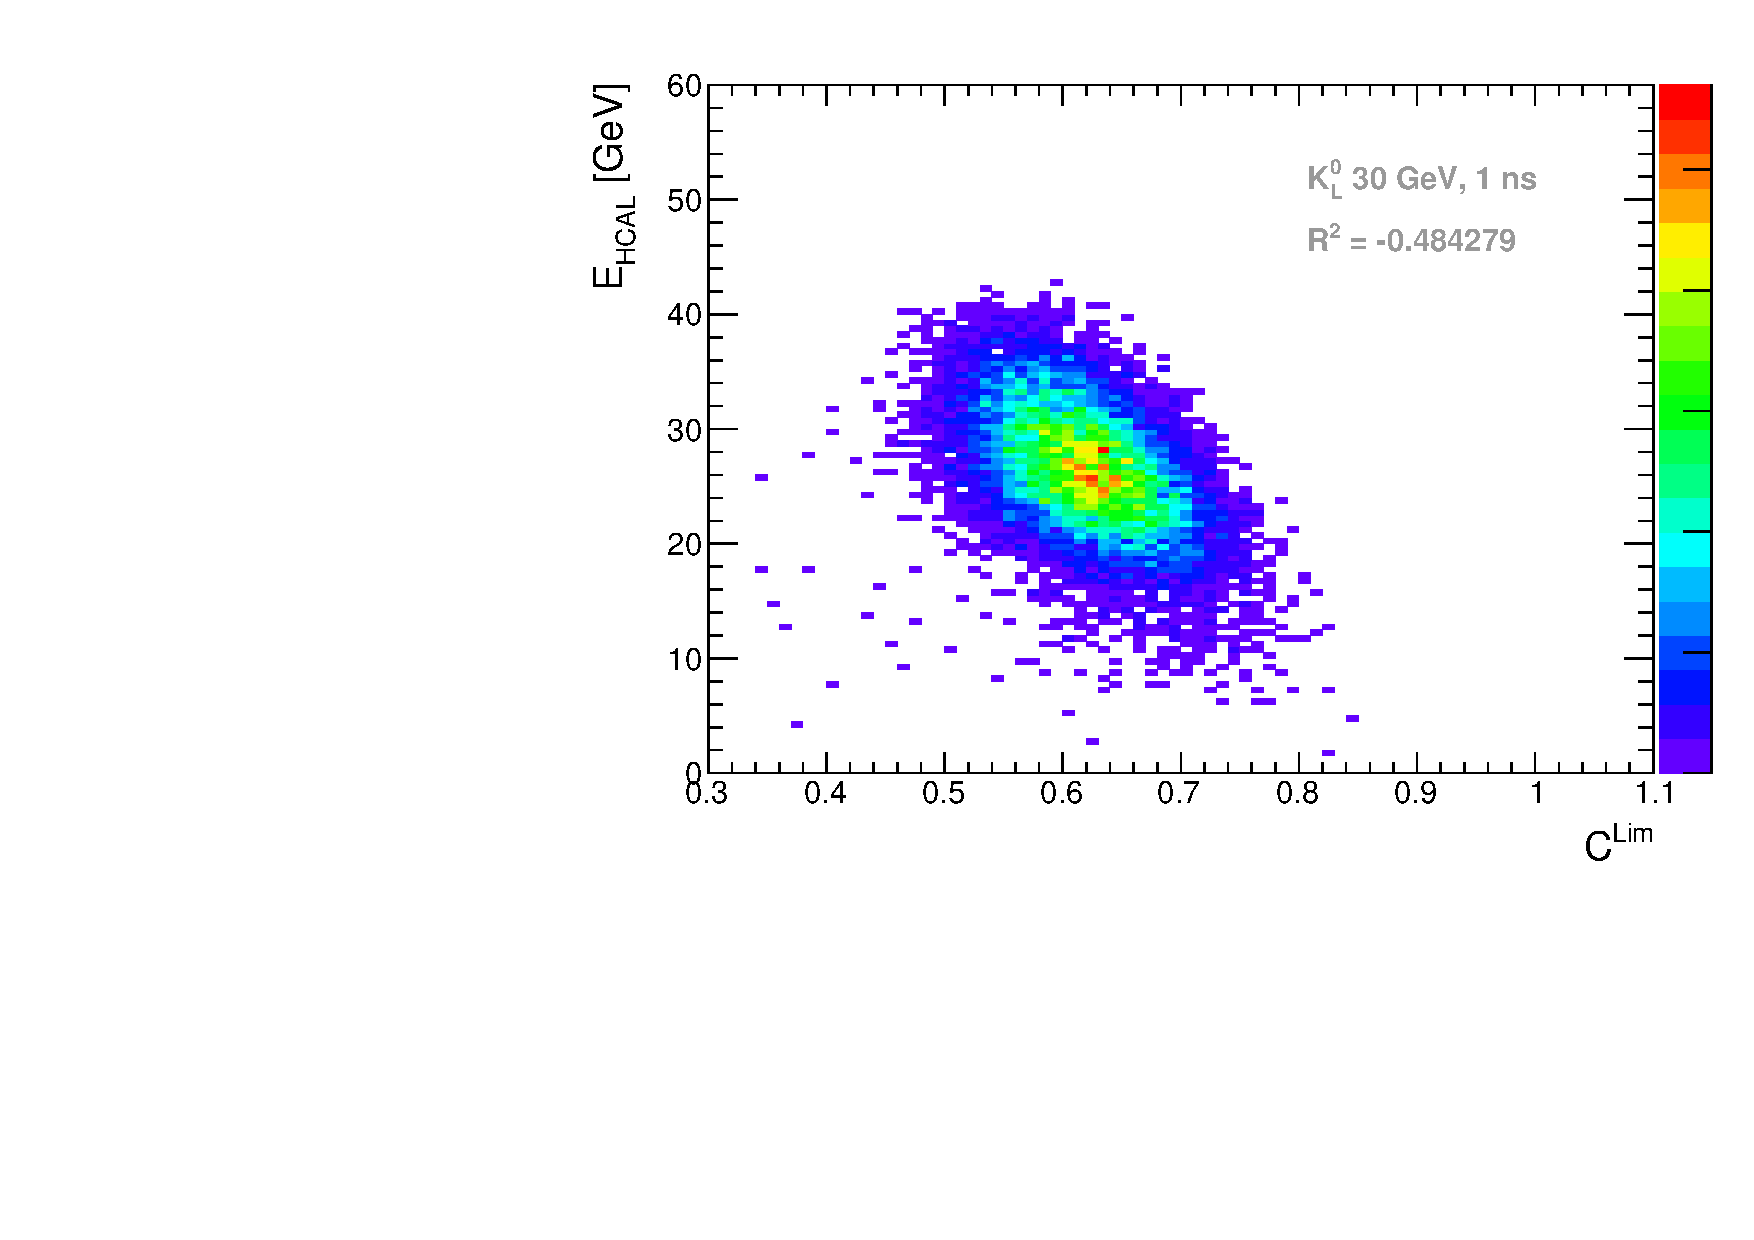
\includegraphics[width=0.7\linewidth]{../Thesis_Plots/ILD/AdditionalPlots/Plots/EhcalCLim_1ns_30GeV.pdf}
  \caption{Correlation between the energy deposited in the HCAL for 30 GeV kaons and $C^{lim}$ for $e^{lim}$ = 3.5 MIPs with a timing cut of 1 ns.} \label{fig:EhcalCLim30_1ns}
\end{figure}
